% CH5103 term-paper presentation (LuaLaTeX). Build: make  (or latexmk main.tex)
\documentclass[aspectratio=169,11pt]{beamer}
\usetheme{Noir}
\usepackage{noir-macros}
\usepackage{minted}
\setminted{fontsize=\scriptsize,style=monokai,breaklines,tabsize=2}
\graphicspath{{figures/}{../assets/figures/}}

\title{Uncommon Molecular Electronic Configurations}
\subtitle{Theory, derivations and verification of Gryn'ova, Coote \& Corminboeuf (2015)}
\author{Shuvam Banerji Seal}
\institute{CH5103 Term Paper}
\date{\today}

\begin{document}
\begin{frame}[plain,noframenumbering]
  \titlepage
\end{frame}

% ============================================================ roadmap + reading guide
\begin{frame}{The journey}{from the Schr\"odinger equation to a sign error in print}
  \centering
  \begin{tikzpicture}[
      stop/.style={draw=noirgold,fill=noirpanel,rounded corners=3pt,minimum width=2.45cm,minimum height=0.72cm,
                   font=\noirgaramond\footnotesize,text=noirfg,align=center},
      path/.style={-{Stealth[length=4pt]},noirmuted,line width=0.7pt}]
    \node[stop] (a) at (0,2.4) {Foundations};
    \node[stop] (b) at (3,2.4) {Spin \&\\antisymmetry};
    \node[stop] (c) at (6,2.4) {Two electrons,\\two orbitals};
    \node[stop] (d) at (9,2.4) {Energies, $J$ \& $K$};
    \node[stop] (e) at (12,2.4) {Hund's rule};
    \node[stop] (f) at (12,0.9) {Static\\correlation};
    \node[stop] (g) at (9,0.9) {Kinetic\\exchange};
    \node[stop] (h) at (6,0.9) {NBMOs \&\\disjointness};
    \node[stop] (i) at (3,0.9) {Spin\\polarisation};
    \node[stop] (j) at (0,0.9) {Exciting\\cases};
    \node[stop] (k) at (0,-0.6) {Koopmans\\\& Janak};
    \node[stop] (l) at (3,-0.6) {Aufbau\\on trial};
    \node[stop] (m) at (6,-0.6) {Quasi-closed\\shells};
    \node[stop,draw=noircyan] (n) at (9,-0.6) {Our\\verification};
    \node[stop,draw=noirgreen] (o) at (12,-0.6) {Verdict};
    \foreach \x/\y in {a/b,b/c,c/d,d/e,e/f,f/g,g/h,h/i,i/j,j/k,k/l,l/m,m/n,n/o}
      \draw[path] (\x) -- (\y);
  \end{tikzpicture}
  \vskip0.3cm
  {\small\cmuted{Every equation is derived step by step; every identity used was checked by SymPy, PySCF or Lean.}}
\end{frame}

\begin{frame}{How to read these slides}
  \begin{columns}[T]
    \column{0.48\textwidth}
    \begin{paperclaim}
      a statement quoted from the review
    \end{paperclaim}
    \begin{assume}
      what a derivation takes for granted
    \end{assume}
    \begin{keyresult}
      what the derivation proves
    \end{keyresult}
    \column{0.48\textwidth}
    \begin{checked}
      how we tested it (script / proof)
    \end{checked}
    \begin{erratum}
      where the paper got it wrong
    \end{erratum}
    \vskip0.2cm
    \centering
    \okpill\ \badpill\ \warnpill\ \partpill
    \vskip0.2cm
    \raggedright\small $E=h+J$ \quad \why{blue italic: why this step follows}\\[2pt]
    \small a \textcolor{noirgold}{\noirgaramond\scshape symbols} strip at the foot of a slide defines its notation
  \end{columns}
  \vskip0.25cm
  \centering{\small Atomic units throughout: $\hbar=m_e=e=4\pi\varepsilon_0=1$, energies in hartree ($\Eh$).}
\end{frame}

% ============================================================ the paper in a nutshell
\section{The paper}

\begin{frame}{The review}
  \begin{columns}[c]
    \column{0.40\textwidth}
    \centering
    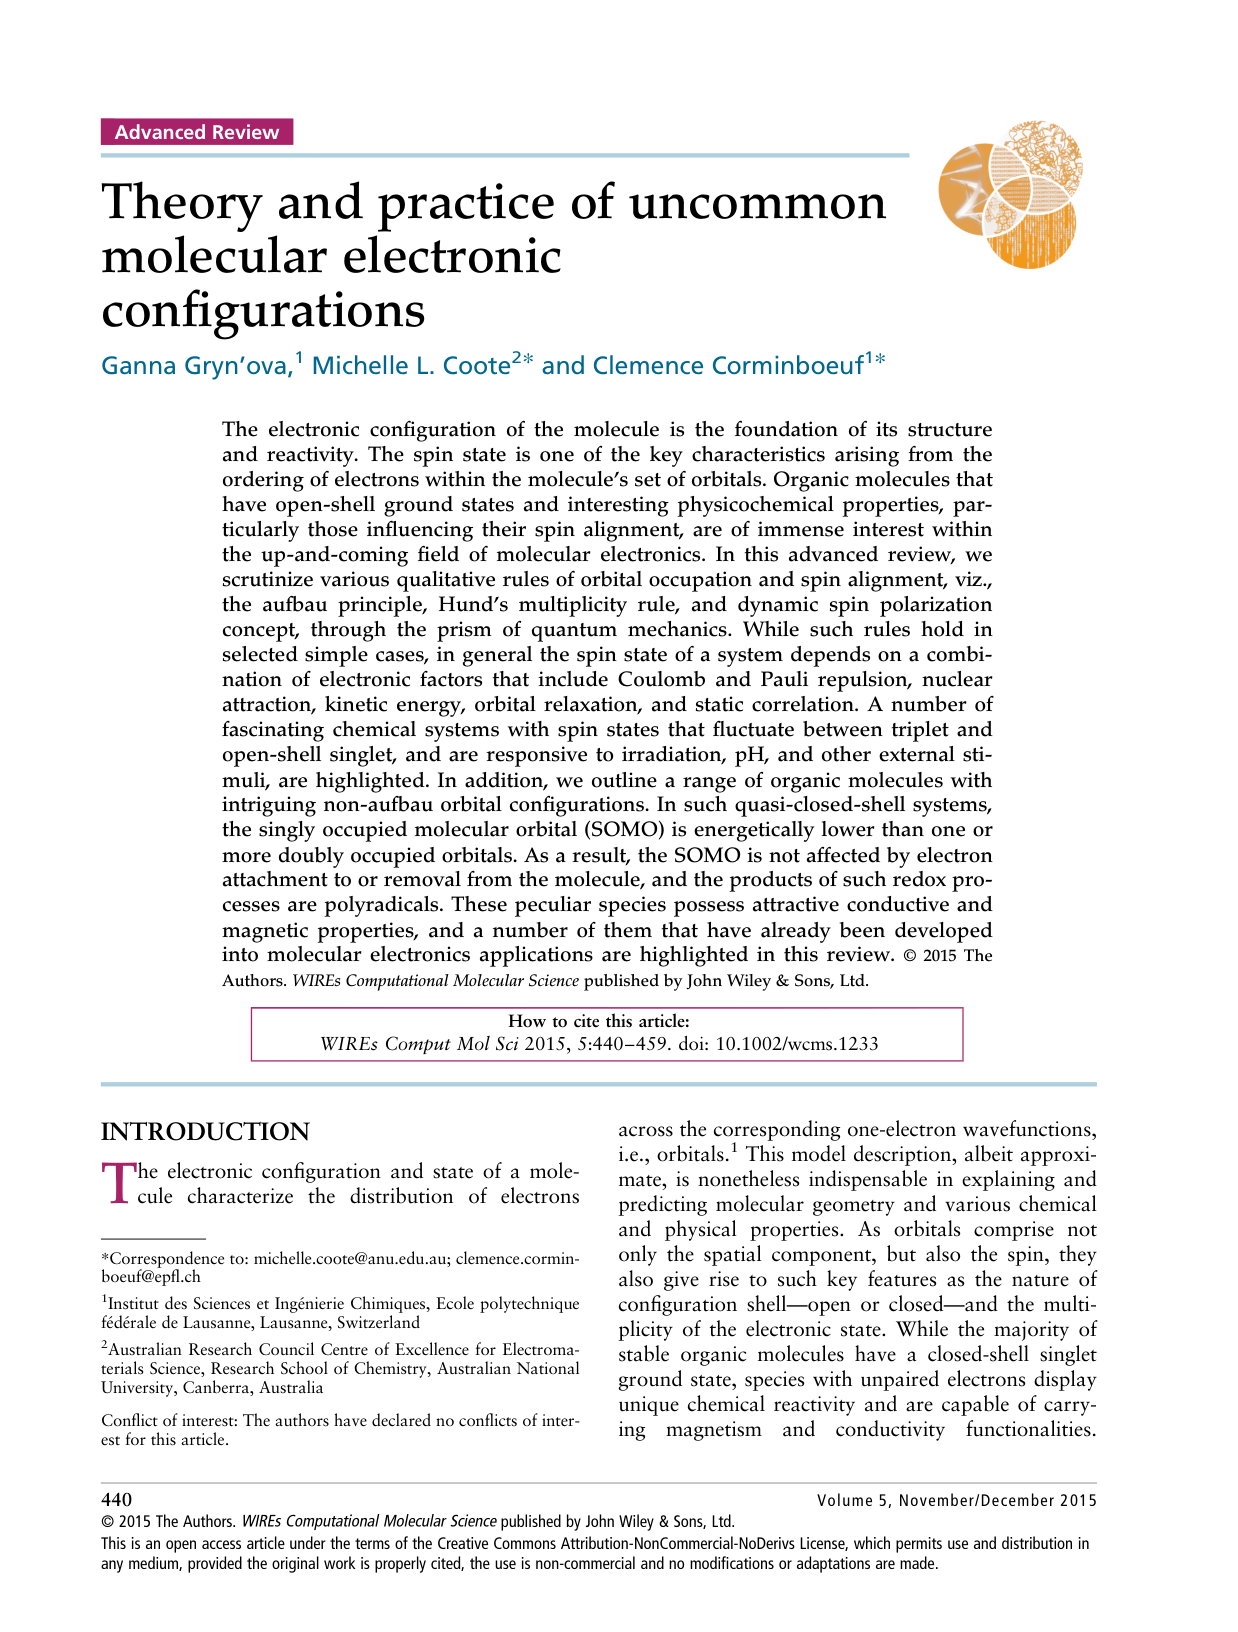
\includegraphics[height=0.74\textheight]{screenshots/paper_page1.png}
    \column{0.58\textwidth}
    {\noircalli\Large\cgold{Theory and practice of uncommon\\ molecular electronic configurations}}
    \vskip0.3cm
    {\noirgaramond Ganna Gryn'ova, Michelle L.\ Coote, Cl\'emence Corminboeuf}
    \vskip0.2cm
    {\small\cmuted{\emph{WIREs Computational Molecular Science} \textbf{5}, 440--459 (2015)\\
      doi:10.1002/wcms.1233 \quad Advanced Review, open access}}
    \vskip0.4cm
    \begin{itemize}
      \item<2-> 20 pages, 17 figures, 5 schemes, 118 references
      \item<3-> part theory (what decides a spin state?)
      \item<4-> part catalogue (molecules that break the textbook rules)
    \end{itemize}
  \end{columns}
\end{frame}

\begin{frame}{Two uncommon configurations}{the two halves of the paper}
  \begin{columns}[T]
    \column{0.48\textwidth}
    \centering{\gsc{1.\ fluctuating multiplicity}}\par\vskip0.2cm
    \begin{tikzpicture}[scale=1.55]
      \begin{scope}
        \orblevel{0}{0}{} \orblevel{0}{0.18}{}
        \elup{0}{0}\elup{0}{0.18}
        \node[font=\scriptsize,text=noirrose] at (0,-0.55) {triplet};
      \end{scope}
      \node[font=\large,text=noirgold] at (1.25,0.1) {vs};
      \begin{scope}[xshift=2.5cm]
        \orblevel{0}{0}{} \orblevel{0}{0.18}{}
        \elup{0}{0}\eldn{0}{0.18}
        \node[font=\scriptsize,text=noirblue] at (0,-0.55) {open-shell singlet};
      \end{scope}
    \end{tikzpicture}
    \vskip0.2cm
    \small two (nearly) degenerate orbitals, two electrons:\\
    \emph{parallel} or \emph{antiparallel}? \\[2pt]
    \onslide<2->{\cgold{Who wins: Hund's rule, or correlation?}}
    \column{0.48\textwidth}
    \centering{\gsc{2.\ non-aufbau ordering}}\par\vskip0.2cm
    \begin{tikzpicture}[scale=1.55]
      \begin{scope}
        \orblevel{0}{1.0}{} \orblevel{0}{0.5}{SOMO} \orblevel{0}{0}{}
        \elup{0}{0.5}\elup{0}{0}\eldn{0}{0}
        \node[font=\scriptsize,text=noirmuted] at (0,-0.55) {aufbau};
      \end{scope}
      \begin{scope}[xshift=2.6cm]
        \orblevel{0}{1.0}{} \orblevel{0}{0.5}{HOMO} \orblevel{0}{0}{SOMO}
        \elup{0}{0.5}\eldn{0}{0.5}\elup{0}{0}
        \node[font=\scriptsize,text=noirrose] at (0,-0.55) {quasi-closed shell};
      \end{scope}
    \end{tikzpicture}
    \vskip0.2cm
    \small the singly occupied orbital lies \emph{below}\\ a doubly occupied one \\[2pt]
    \onslide<3->{\cgold{Oxidation then makes a diradical.}}
  \end{columns}
\end{frame}

\begin{frame}{Why anyone cares}
  \begin{columns}[c]
    \column{0.5\textwidth}
    \small
    \begin{paperclaim}
      ``species with unpaired electrons display unique chemical reactivity and are capable of carrying
      magnetism and conductivity functionalities'' (p.\ 440)
    \end{paperclaim}
    \begin{itemize}
      \item<2-> spin valves, switches, field-effect transistors, logic
      \item<3-> wanted: a set spin state that a stimulus can flip
      \item<4-> but few radicals are persistent, crystallisable \emph{and} not Mott insulators
    \end{itemize}
    \column{0.45\textwidth}
    \centering
    \begin{tikzpicture}[scale=0.8]
      \node[draw=noircyan,rounded corners,fill=noirpanel,minimum width=2.2cm,minimum height=0.8cm,font=\small] (mol) at (0,0) {molecule};
      \foreach \ang/\lab/\col in {90/light/noirgold,30/pH/noirgreen,-30/redox/noirrose,-90/heat/noirorange,210/field/noirblue,150/metal ion/noirviolet}
        \node[font=\scriptsize,text=\col] (s\ang) at (\ang:2.1) {\lab};
      \foreach \ang in {90,30,-30,-90,210,150}
        \draw[-{Stealth[length=4pt]},noirmuted] (s\ang) -- (mol);
      \node[font=\scriptsize,text=noirmuted,align=center] at (0,-2.75) {stimuli that switch spin states\\(Figures 7--9 of the review)};
    \end{tikzpicture}
  \end{columns}
\end{frame}

\begin{frame}{What we did with it}
  \centering
  \begin{tikzpicture}
    \node[noirbox=noirgold] (read) at (0,0) {read\\{\scriptsize 20 pp., 118 refs}};
    \node[noirbox=noirviolet] (der) at (3.2,0) {derive\\{\scriptsize 18 sections}};
    \node[noirbox=noircyan] (num) at (6.4,0.9) {compute\\{\scriptsize PySCF, SymPy, ED}};
    \node[noirbox=noircyan] (lean) at (6.4,-0.9) {prove\\{\scriptsize Lean 4 + Mathlib}};
    \node[noirbox=noirgreen] (ver) at (9.6,0) {verdict\\{\scriptsize claim by claim}};
    \draw[noirarr] (read) -- (der);
    \draw[noirarr] (der) -- (num); \draw[noirarr] (der) -- (lean);
    \draw[noirarr] (num) -- (ver); \draw[noirarr] (lean) -- (ver);
    \node<2->[font=\scriptsize,text=noirmuted,align=center] at (6.4,-2.15) {19 tests (T1--T17)\\17 machine-checked theorems};
    \node<3->[font=\scriptsize,text=noirrose,align=center] at (9.6,-1.5) {\ldots and one\\published sign error};
  \end{tikzpicture}
\end{frame}

% ============================================================ foundations
\section{Foundations}

\begin{frame}{Where everything starts}{the molecular Schr\"odinger equation}
  \[
    \Hop_{\text{mol}}\,\Psi=E\,\Psi
  \]
  \vskip-0.2cm
  \[
    \Hop_{\text{mol}}=
    \underbrace{-\sum_A\frac{\nabla_A^2}{2M_A}}_{\onslide<2->{\cmuted{\text{nuclear KE}}}}
    \underbrace{-\sum_i\frac{\nabla_i^2}{2}}_{\onslide<3->{\ccyan{\text{electron KE}}}}
    \underbrace{-\sum_{i,A}\frac{Z_A}{r_{iA}}}_{\onslide<4->{\cgold{\text{e--n attraction}}}}
    \underbrace{+\sum_{i<j}\frac{1}{r_{ij}}}_{\onslide<5->{\crose{\text{e--e repulsion}}}}
    \underbrace{+\sum_{A<B}\frac{Z_AZ_B}{R_{AB}}}_{\onslide<6->{\cmuted{\text{n--n repulsion}}}}
  \]
  \vskip0.2cm
  \begin{center}
  \begin{tikzpicture}[scale=1.15]
    \fill[noirgold] (0,0) circle (0.13) node[below=3pt,font=\scriptsize,text=noirgold]{$A$};
    \fill[noirgold] (4,0) circle (0.13) node[below=3pt,font=\scriptsize,text=noirgold]{$B$};
    \fill[noircyan] (1.3,1.2) circle (0.07) node[above,font=\scriptsize,text=noircyan]{$i$};
    \fill[noircyan] (2.9,1.0) circle (0.07) node[above,font=\scriptsize,text=noircyan]{$j$};
    \onslide<4->{\draw[noirgold,dashed] (0,0) -- (1.3,1.2) node[midway,left,font=\tiny]{$r_{iA}$};}
    \onslide<5->{\draw[noirrose] (1.3,1.2) -- (2.9,1.0) node[midway,above,font=\tiny]{$r_{ij}$};}
    \onslide<6->{\draw[noirmuted,dashed] (0,0) -- (4,0) node[midway,below,font=\tiny]{$R_{AB}$};}
  \end{tikzpicture}
  \end{center}
\end{frame}

\begin{frame}{Born--Oppenheimer: freeze the nuclei}
  \begin{assume}
    $M_A\gg m_e=1$: electrons adjust instantly to nuclear positions; treat $\{\mathbf R_A\}$ as parameters.
  \end{assume}
  \begin{enumerate}
    \item<2-> drop the nuclear kinetic energy \hfill $-\sum_A\nabla_A^2/2M_A\to0$
    \item<3-> nuclear repulsion becomes a constant \hfill $V_{nn}(\mathbf R)$
    \item<4-> what is left is the \cgold{electronic Hamiltonian}
  \end{enumerate}
  \onslide<4->{
  \[
    \boxed{\;\Hop=\sum_{i=1}^{N}\hat h(i)+\sum_{i<j}\frac1{r_{ij}},\qquad
    \hat h(i)=-\tfrac12\nabla_i^2-\sum_A\frac{Z_A}{r_{iA}}\;}
  \]}
  \onslide<5->{\centering\small $\hat h$ acts on one electron at a time;
    \crose{$1/r_{ij}$ couples every pair}: that coupling is what this whole paper is about.\par}
  \onslide<6->{\centering\small \cmuted{Note: $\Hop$ contains no spin. Spin will enter only through the Pauli principle.}\par}
\end{frame}

\begin{frame}{The variational principle}{why ``lower energy'' means ``better wavefunction''}
  {\small\cviolet{Assume:} exact eigenstates $\Hop\Psi_n=E_n\Psi_n$, orthonormal, complete, $E_0\le E_1\le\cdots$}
  {\large\begin{align*}
    \stepno{1}\ \tilde\Psi&=\textstyle\sum_n c_n\Psi_n,\qquad \sum_n|c_n|^2=1 &&\cmuted{\text{expand any trial function}}\\
    \uncover<2->{\stepno{2}\ \langle\tilde\Psi|\Hop|\tilde\Psi\rangle}&\uncover<2->{=\textstyle\sum_{m,n}c_m^*c_n\,E_n\langle\Psi_m|\Psi_n\rangle}
      &&\uncover<2->{\cmuted{\text{$\Hop$ acts on $\Psi_n$}}}\\
    &\uncover<3->{=\textstyle\sum_n|c_n|^2E_n} &&\uncover<3->{\cmuted{\langle\Psi_m|\Psi_n\rangle=\delta_{mn}}}\\
    \uncover<4->{\stepno{3}}&\uncover<4->{\ge\textstyle\sum_n|c_n|^2E_0=E_0} &&\uncover<4->{\cmuted{E_n\ge E_0}}
  \end{align*}}
  \onslide<5->{
  \begin{keyresult}
    $E[\tilde\Psi]\ge E_0$ for every normalised $\tilde\Psi$; Hartree--Fock and CI rest on it.
  \end{keyresult}}
\end{frame}

\begin{frame}{Orbitals: the independent-electron picture}
  \begin{columns}[T]
    \column{0.55\textwidth}
    \begin{assume}[Independent-particle model]
      replace $\sum_{i<j}1/r_{ij}$ by an \emph{average} field felt by each electron
    \end{assume}
    \onslide<2->{\[
      \hat f\,\varphi_p=\varepsilon_p\,\varphi_p\qquad\text{(one-electron problem)}
    \]}
    \onslide<3->{LCAO: expand in atom-centred functions
    \[
      \varphi_p(\mathbf r)=\sum_\mu c_{\mu p}\,\chi_\mu(\mathbf r)
    \]}
    \onslide<4->{\small orbital = one-electron wavefunction; its \emph{energy} $\varepsilon_p$ and its \emph{occupation} build the configuration.}
    \column{0.42\textwidth}
    \centering
    \begin{tikzpicture}[scale=1.25]
      \draw[-{Stealth[length=4pt]},noirmuted] (-0.2,-0.1) -- (-0.2,3.2) node[above,font=\scriptsize]{$\varepsilon$};
      \orblevel{0.8}{0.2}{$\varphi_1$}\orblevel{0.8}{0.9}{$\varphi_2$}\orblevel{0.8}{1.6}{$\varphi_3$}\orblevel{0.8}{2.5}{$\varphi_4$}
      \onslide<4->{\elup{0.8}{0.2}\eldn{0.8}{0.2}\elup{0.8}{0.9}\eldn{0.8}{0.9}\elup{0.8}{1.6}}
      \onslide<4->{\node[font=\tiny,text=noirgold,anchor=west] at (1.6,1.6) {SOMO};}
    \end{tikzpicture}
  \end{columns}
\end{frame}

\begin{frame}{Box 1: ``Much ado about orbitals''}
  \begin{columns}[c]
    \column{0.55\textwidth}
    \begin{paperclaim}
      ``The reality is that an orbital is a mathematical construct, an approximate, non-unique solution
      to the Schr\"odinger equation.''
    \end{paperclaim}
    \onslide<2->{
    \begin{plainpanel}
      \small
      \cgold{Non-unique:} any unitary mixing of occupied orbitals leaves the determinant (and every
      observable) unchanged. \\[3pt]
      \cgold{Approximate:} orbitals exist only inside the independent-particle model.
    \end{plainpanel}}
    \column{0.4\textwidth}
    \raggedright
    \onslide<3->{
    \begin{plainpanel}
      \small
      The 1999 \emph{Nature} report of ``direct observation of d-orbital holes'' in Cu$_2$O started a debate:
      \emph{can an orbital be observed?}\par\smallskip
      \cmuted{What is observable is the density $\rho(\mathbf r)$, and orbital \emph{occupations}.}
    \end{plainpanel}}
  \end{columns}
  \vskip0.2cm
  \onslide<4->{\centering\small\cgold{Keep this in mind: it returns when ROHF orbital energies turn out to be arbitrary.}\par}
\end{frame}

% ============================================================ antisymmetry and spin
\section{Spin \& antisymmetry}

\begin{frame}{Swapping two electrons}{why the exchange eigenvalue is $\pm1$}
  \begin{columns}[c]
    \column{0.62\textwidth}
    Define $\hat P_{12}\Psi(x_1,x_2)=\Psi(x_2,x_1)$, \quad $x=(\mathbf r,\sigma)$.
    {\begin{align*}
      \stepno{1}\ &\hat P_{12}^2=\hat 1 &&\why{swapping twice restores the order}\\
      \uncover<2->{\stepno{2}\ }&\uncover<2->{\hat P_{12}\Psi=\lambda\Psi\ \Rightarrow\ \Psi=\lambda^2\Psi} &&\uncover<2->{\why{apply $\hat P_{12}$ twice}}\\
      \uncover<3->{\stepno{3}\ }&\uncover<3->{\lambda=\pm1} &&\uncover<3->{\why{since $\lambda^2=1$}}\\
      \uncover<4->{\stepno{4}\ }&\uncover<4->{[\Hop,\hat P_{12}]=0} &&\uncover<4->{\why{$\Hop$ treats all electrons alike}}
    \end{align*}}
    \column{0.34\textwidth}
    \centering
    \begin{tikzpicture}[scale=1.0]
      \fill[noircyan] (0,0) circle (0.12) node[below=3pt,font=\scriptsize]{1};
      \fill[noirrose] (2,0) circle (0.12) node[below=3pt,font=\scriptsize]{2};
      \draw[-{Stealth[length=5pt]},noirgold,line width=0.8pt] (0.2,0.15) to[bend left=50] (1.8,0.15);
      \draw[-{Stealth[length=5pt]},noirgold,line width=0.8pt] (1.8,-0.15) to[bend left=50] (0.2,-0.15);
      \node[font=\small,text=noirgold] at (1,0.95) {$\hat P_{12}$};
      \onslide<5->{\node[font=\large,text=noirrose] at (1,-1.15) {$\lambda=-1$};}
    \end{tikzpicture}
  \end{columns}
  \onslide<5->{\small\cgold{so eigenstates have definite $\lambda$; for electrons nature picks $-1$.} The paper: ``the wavefunction for a
    system of fermions must be antisymmetric with respect to the interchange of any two particles'' (p.\ 441)\par}
  \symbolstrip{$x_i=(\mathbf r_i,\sigma_i)$: all coordinates of electron $i$, position $\mathbf r_i$ plus spin coordinate $\sigma_i$ ($\uparrow$ or $\downarrow$)
    \quad $\hat P_{12}$: operator exchanging electrons 1 and 2 \quad $\lambda$: its eigenvalue \quad $[\hat A,\hat B]=\hat A\hat B-\hat B\hat A$
    \quad fermions: half-integer-spin particles (electrons)}
\end{frame}

\begin{frame}{Slater determinants}{antisymmetry built in}
  \[
    D[\chi_1,\chi_2]=\begin{vmatrix}\chi_1(1)&\chi_2(1)\\\chi_1(2)&\chi_2(2)\end{vmatrix}
    =\chi_1(1)\chi_2(2)-\chi_2(1)\chi_1(2)
  \]
  \vskip-0.2cm
  \explain{rows label electrons, columns label spin orbitals; the determinant mixes every assignment with a sign}
  \begin{itemize}
    \item<2-> swap electrons $\Leftrightarrow$ swap two \emph{rows} $\Rightarrow$ $D\to-D$ \hfill\cgreen{antisymmetric}
    \item<3-> two equal spin orbitals $\Leftrightarrow$ two equal \emph{columns} $\Rightarrow$ $D=0$ \hfill\cgold{Pauli exclusion}
    \item<4-> normalised: $\ket{\chi_1\chi_2}=\tfrac1{\sqrt2}D[\chi_1,\chi_2]$
  \end{itemize}
  \onslide<5->{
  \begin{keyresult}
    Pauli's 1925 rule (no two electrons with all four quantum numbers equal; p.\ 448) is a \emph{consequence}
    of antisymmetry inside the orbital model, not a separate law.
  \end{keyresult}}
  \symbolstrip{$\chi(x)$: spin orbital $=$ spatial orbital $\times$ spin function, e.g.\ $\chi=\pa(\mathbf r)\,\alpha(\sigma)$ \quad
    $\chi_1(2)$: spin orbital 1 at electron 2's coordinates \quad $\tfrac1{\sqrt2}$: $D$ is two orthogonal products of norm 1, so $\braket DD=2$}
\end{frame}

\begin{frame}{Spin operators for two electrons}
  \begin{columns}[T]
    \column{0.47\textwidth}
    \cgold{One electron} ($s=\tfrac12$):
    {\begin{align*}
      \hat s_z\alpha&=+\tfrac12\alpha, & \hat s_z\beta&=-\tfrac12\beta\\
      \hat s_+\beta&=\alpha, & \hat s_+\alpha&=0\\
      \hat s_-\alpha&=\beta, & \hat s_-\beta&=0
    \end{align*}}
    \onslide<2->{\cgold{Two electrons:} add each electron's operator\par
      $\hat S_z=\hat s_{z}(1)+\hat s_{z}(2)$,\ \ $\hat S_\pm=\hat s_\pm(1)+\hat s_\pm(2)$}
    \column{0.5\textwidth}
    \onslide<3->{\cgold{A useful identity:}}
    {\begin{align*}
      \uncover<3->{\hat S_-\hat S_+}&\uncover<3->{=(\hat S_x-i\hat S_y)(\hat S_x+i\hat S_y)} &&\uncover<3->{\why{definition of $\hat S_\pm$}}\\
      &\uncover<4->{=\hat S_x^2+\hat S_y^2+i[\hat S_x,\hat S_y]} &&\uncover<4->{\why{multiply out}}\\
      &\uncover<5->{=\hat S^2-\hat S_z^2+i(i\hat S_z)} &&\uncover<5->{\why{$[\hat S_x,\hat S_y]=i\hat S_z$}}\\
      &\uncover<6->{=\hat S^2-\hat S_z^2-\hat S_z} &&\uncover<6->{\why{$i\cdot i=-1$}}
    \end{align*}}
    \onslide<7->{\[
      \boxed{\hat S^2=\hat S_-\hat S_++\hat S_z^2+\hat S_z}
    \]}
  \end{columns}
  \symbolstrip{$\alpha,\beta$: spin up / down of one electron \quad $\hat s_+$ flips $\downarrow\to\uparrow$, $\hat s_-$ flips $\uparrow\to\downarrow$ (0 if impossible)
    \quad $\hat S_x,\hat S_y,\hat S_z,\hat S^2$: total spin components and squared magnitude \quad $\hbar=1$}
\end{frame}

\begin{frame}{$\hat S^2$ on the four spin products (1/2)}
  \begin{columns}[T]
    \column{0.48\textwidth}
    \cgold{$\alpha_1\alpha_2$} \ \cmuted{(both up)}
    {\begin{align*}
      \hat S_+\alpha_1\alpha_2&=0 &&\why{nothing left to raise}\\
      \uncover<2->{\hat S_z\alpha_1\alpha_2}&\uncover<2->{=(\tfrac12+\tfrac12)\alpha_1\alpha_2} &&\uncover<2->{\why{each adds $+\tfrac12$}}\\
      \uncover<3->{\hat S^2\alpha_1\alpha_2}&\uncover<3->{=(0+1+1)\,\alpha_1\alpha_2} &&\uncover<3->{\why{$\hat S_-\hat S_+ +\hat S_z^2+\hat S_z$}}\\
      &\uncover<4->{=\cgreen{2}\,\alpha_1\alpha_2}
    \end{align*}}
    \onslide<4->{\small $S(S+1)=2\Rightarrow S=1,\ M_S=+1$}
    \column{0.48\textwidth}
    \onslide<5->{\cgold{$\beta_1\beta_2$} \ \cmuted{(both down)}}
    {\begin{align*}
      \uncover<5->{\hat S_+\beta_1\beta_2}&\uncover<5->{=\alpha_1\beta_2+\beta_1\alpha_2} &&\uncover<5->{\why{raise 1 or 2}}\\
      \uncover<6->{\hat S_-(\ldots)}&\uncover<6->{=\beta_1\beta_2+\beta_1\beta_2} &&\uncover<6->{\why{lower the raised one}}\\
      \uncover<7->{(\hat S_z^2+\hat S_z)\beta_1\beta_2}&\uncover<7->{=(1-1)\beta_1\beta_2} &&\uncover<7->{\why{$M_S=-1$}}\\
      \uncover<8->{\hat S^2\beta_1\beta_2}&\uncover<8->{=\cgreen{2}\,\beta_1\beta_2}
    \end{align*}}
    \onslide<8->{\small $S=1,\ M_S=-1$}
  \end{columns}
  \symbolstrip{$\alpha_1\equiv\alpha(\sigma_1)$: electron 1 is spin up \quad $\alpha_1\beta_2$: electron 1 up, electron 2 down
    \quad eigenvalue of $\hat S^2$ is $S(S+1)$ \quad $M_S$: eigenvalue of $\hat S_z$ (sum of the two $\pm\tfrac12$)}
\end{frame}

\begin{frame}{$\hat S^2$ on the four spin products (2/2)}
  \cgold{$\alpha_1\beta_2$ and $\beta_1\alpha_2$} \quad\cmuted{($M_S=0$; neither is an eigenfunction on its own)}
  {\begin{align*}
    \hat S_+\alpha_1\beta_2&=\alpha_1\alpha_2 &
    \uncover<2->{\hat S_-\alpha_1\alpha_2}&\uncover<2->{=\beta_1\alpha_2+\alpha_1\beta_2}\\
    \uncover<3->{\hat S_z\alpha_1\beta_2}&\uncover<3->{=(\tfrac12-\tfrac12)\,\alpha_1\beta_2=0} &
    \uncover<4->{\Rightarrow\ \hat S^2\alpha_1\beta_2}&\uncover<4->{=\alpha_1\beta_2+\beta_1\alpha_2}\\
    &&\uncover<5->{\hat S^2\beta_1\alpha_2}&\uncover<5->{=\alpha_1\beta_2+\beta_1\alpha_2\quad\why{same steps}}
  \end{align*}}
  \explain<4->{$\hat S^2$ turns $\alpha_1\beta_2$ into a \emph{different} function: it is not an eigenfunction}
  \onslide<6->{Add and subtract the two results:}
  \[
    \uncover<6->{\hat S^2(\alpha_1\beta_2\pm\beta_1\alpha_2)=(1\pm1)\,(\alpha_1\beta_2\pm\beta_1\alpha_2)}
  \]
  \onslide<7->{\centering
  \begin{tikzpicture}
    \node[draw=noirrose,rounded corners,fill=noirpanel,inner sep=5pt] at (0,0) {$+$:\ eigenvalue $2$\ \ $\Rightarrow S=1$};
    \node[draw=noirblue,rounded corners,fill=noirpanel,inner sep=5pt] at (5.2,0) {$-$:\ eigenvalue $0$\ \ $\Rightarrow S=0$};
  \end{tikzpicture}\par}
  \symbolstrip{$\hat S_+$ acts on electron 1 or 2 in turn (it is a sum); only the $\beta$ of electron 2 can be raised here \quad
    $(1\pm1)$: $1+1=2$ for the sum, $1-1=0$ for the difference}
\end{frame}

\begin{frame}{Triplet and singlet spin functions}
  \begin{columns}[c]
    \column{0.6\textwidth}
    \begin{keyresult}[The four two-electron spin states]
      \vskip-0.6em
      {\begin{align*}
        \Theta_{1,+1}&=\alpha_1\alpha_2\\
        \Theta_{1,0}&=\tfrac1{\sqrt2}(\alpha_1\beta_2+\beta_1\alpha_2)\\
        \Theta_{1,-1}&=\beta_1\beta_2\\
        \Theta_{0,0}&=\tfrac1{\sqrt2}(\alpha_1\beta_2-\beta_1\alpha_2)
      \end{align*}}
    \end{keyresult}
    \explain{$\tfrac1{\sqrt2}$: the two products are orthonormal, so the sum has norm$^2$ 2}
    \column{0.36\textwidth}
    \begin{itemize}
      \item<2-> triplet spin functions are \cgold{symmetric} under $1\leftrightarrow2$
      \item<3-> the singlet is \cgold{antisymmetric}
      \item<4-> total must be antisymmetric, so
    \end{itemize}
    \onslide<4->{
    \begin{center}
      \small
      \begin{tabular}{lcc}
        \toprule & space & spin\\\midrule
        triplet & \crose{anti} & sym\\
        singlet & \cblue{sym} & anti\\\bottomrule
      \end{tabular}
    \end{center}}
  \end{columns}
  \onslide<5->{\centering\small\tick\ \cmuted{T1: $\hat S^2,\hat S_z$ as $4\times4$ matrices in SymPy; all eigen-relations exact.}\par}
  \symbolstrip{$\Theta_{S,M_S}$: two-electron spin function with total spin $S$ and projection $M_S$ \quad
    symmetric: unchanged when $1\leftrightarrow2$; antisymmetric: changes sign \quad (anti)$\times$(sym) $=$ anti, as required}
\end{frame}

% ============================================================ two electrons in two orbitals + the sign error
\section{Two electrons, two orbitals}

\begin{frame}{Six ways to place two electrons}{Figure 1 of the review, rebuilt}
  \centering
  \begin{tikzpicture}[scale=1.15]
    \foreach \lab/\x/\ms in {i/0/0,ii/1.6/0,iii/3.2/0,iv/4.8/0,v/6.4/{+1},vi/8.0/{-1}}{
      \node[font=\small\itshape,text=noirgold] at (\x,1.85) {\lab};
      \draw[level] (\x-0.4,0) -- (\x+0.4,0);
      \draw[level] (\x-0.4,1.1) -- (\x+0.4,1.1);
      \node[font=\small,text=noirmuted] at (\x,-0.7) {$M_S=\ms$};
    }
    \node[font=\small,text=noirfg] at (-0.95,0) {$\pa$};
    \node[font=\small,text=noirfg] at (-0.95,1.1) {$\pb$};
    \onslide<2->{\elup{0}{0}\eldn{0}{0}}
    \onslide<3->{\elup{1.6}{1.1}\eldn{1.6}{1.1}}
    \onslide<4->{\elup{3.2}{0}\eldn{3.2}{1.1}}
    \onslide<5->{\eldn{4.8}{0}\elup{4.8}{1.1}}
    \onslide<6->{\elup{6.4}{0}\elup{6.4}{1.1}}
    \onslide<7->{\eldn{8.0}{0}\eldn{8.0}{1.1}}
    \onslide<8->{
      \draw[decorate,decoration={brace,amplitude=5pt,mirror},noirblue] (-0.45,-1.0) -- (1.95,-1.0)
        node[midway,below=6pt,font=\scriptsize,text=noirblue]{closed shells};
      \draw[decorate,decoration={brace,amplitude=5pt,mirror},noirviolet] (2.75,-1.0) -- (5.25,-1.0)
        node[midway,below=6pt,font=\scriptsize,text=noirviolet]{open shell, $M_S=0$};
      \draw[decorate,decoration={brace,amplitude=5pt,mirror},noirrose] (5.95,-1.0) -- (8.45,-1.0)
        node[midway,below=6pt,font=\scriptsize,text=noirrose]{high spin};}
  \end{tikzpicture}
  \vskip0.1cm
  \onslide<8->{\small four spin orbitals $\pa\alpha,\pa\beta,\pb\alpha,\pb\beta$; choose 2 of 4 \;$\Rightarrow$\; $\binom42=6$ determinants}
  \symbolstrip{$\pa,\pb$: the two spatial orbitals (real, orthonormal), e.g.\ the two frontier orbitals of a diradical \quad
    \textcolor{noirrose}{$\uparrow$}/\textcolor{noirblue}{$\downarrow$}: electron with spin $\alpha$/$\beta$ \quad
    $M_S$: total $S_z$ $=$ sum of $+\tfrac12$ per $\uparrow$ and $-\tfrac12$ per $\downarrow$}
\end{frame}

\begin{frame}{The paper's Figure 1}
  \begin{columns}[c]
    \column{0.55\textwidth}
    \centering
    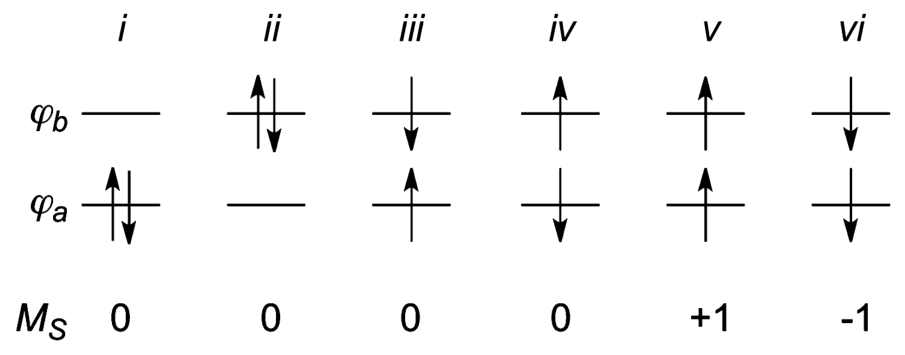
\includegraphics[width=\linewidth]{fig01_two_electron_determinants.png}
    \column{0.42\textwidth}
    \begin{paperclaim}
      ``Various arrangements (determinants) of two electrons in two molecular orbitals and the corresponding
      values of the secondary spin quantum number.'' (p.\ 441)
    \end{paperclaim}
    \onslide<2->{\small\cgreen{Matches our reconstruction.} Now write each one out.}
  \end{columns}
  \symbolstrip{``secondary spin quantum number'' $=M_S$, the projection of the total spin on the $z$ axis}
\end{frame}

\begin{frame}{Writing the determinants out}
  \small
  shorthand: \quad $\ccyan{A}\equiv\pa(1)\pb(2)$ \cmuted{(electron 1 in $\pa$, 2 in $\pb$)},\qquad
  $\crose{B}\equiv\pb(1)\pa(2)$ \cmuted{(swapped)}
  \vskip0.1cm
  \begin{center}
  \renewcommand{\arraystretch}{1.2}
  \begin{tabular}{@{}l l l@{}}
    \toprule
    & spin orbitals $\chi_1,\chi_2$ & $D=\chi_1(1)\chi_2(2)-\chi_2(1)\chi_1(2)$\\
    \midrule
    i   & $\pa\alpha,\ \pa\beta$ & $\pa(1)\pa(2)\,(\alpha_1\beta_2-\beta_1\alpha_2)$\\
    ii  & $\pb\alpha,\ \pb\beta$ & $\pb(1)\pb(2)\,(\alpha_1\beta_2-\beta_1\alpha_2)$\\
    \onslide<2->{iii} & \onslide<2->{$\pa\alpha,\ \pb\beta$} & \onslide<2->{$\ccyan{A}\,\alpha_1\beta_2-\crose{B}\,\beta_1\alpha_2$}\\
    \onslide<3->{iv}  & \onslide<3->{$\pa\beta,\ \pb\alpha$} & \onslide<3->{$\ccyan{A}\,\beta_1\alpha_2-\crose{B}\,\alpha_1\beta_2$}\\
    \onslide<4->{v}   & \onslide<4->{$\pa\alpha,\ \pb\alpha$} & \onslide<4->{$(\ccyan{A}-\crose{B})\,\alpha_1\alpha_2$}\\
    \onslide<4->{vi}  & \onslide<4->{$\pa\beta,\ \pb\beta$} & \onslide<4->{$(\ccyan{A}-\crose{B})\,\beta_1\beta_2$}\\
    \bottomrule
  \end{tabular}
  \end{center}
  \onslide<2->{\cmuted{e.g.\ iii: }$\chi_1=\pa\alpha,\ \chi_2=\pb\beta$:\quad
  $\pa(1)\alpha_1\,\pb(2)\beta_2-\pb(1)\beta_1\,\pa(2)\alpha_2$}
  \explain<2->{in each product the spatial part and the spin part of the same electron travel together}
  \symbolstrip{$D_{\text{X}}$: \emph{unnormalised} determinant of row X (its normalised form is $\tfrac1{\sqrt2}D$) \quad
    $\pa(1)$: orbital $\pa$ evaluated at electron 1's position $\mathbf r_1$ \quad $\alpha_1\beta_2$: electron 1 up, electron 2 down}
\end{frame}

\begin{frame}{$M_S=\pm1$: one determinant each}
  \begin{align*}
    \tfrac1{\sqrt2}D_{\text v}&=\underbrace{\tfrac1{\sqrt2}\bigl[\pa(1)\pb(2)-\pb(1)\pa(2)\bigr]}_{\text{antisymmetric space}}\;
      \underbrace{\alpha_1\alpha_2}_{\Theta_{1,+1}} &&\why{row v: $(A-B)\,\alpha_1\alpha_2$}\\
    \uncover<2->{\tfrac1{\sqrt2}D_{\text{vi}}}&\uncover<2->{=\tfrac1{\sqrt2}\bigl[\pa(1)\pb(2)-\pb(1)\pa(2)\bigr]\;\beta_1\beta_2}
      &&\uncover<2->{\why{same space, both spins down}}
  \end{align*}
  \onslide<3->{
  \begin{paperclaim}
    ``$^3\Psi(M_s=+1)=\tfrac1{\sqrt2}[\pa(1)\pb(2)-\pb(1)\pa(2)][\alpha_1\alpha_2]$'' \dots\ ``i.e., they can be
    represented as single determinants v and vi'' (p.\ 441; $M_s=-1$ analogous with $\beta_1\beta_2$)
  \end{paperclaim}}
  \onslide<4->{\centering\okpill\quad\small exactly right: the high-spin triplet components are \cgold{single-reference}.\par}
  \symbolstrip{$^3\Psi$: triplet ($2S+1=3$) \quad one determinant already factorises into (space)$\times$(spin of definite $S$) \quad
    $\tfrac1{\sqrt2}$ normalises $A-B$, since $\braket{A-B}{A-B}=2$}
\end{frame}

\begin{frame}{$M_S=0$: iii and iv are not spin eigenfunctions}
  \begin{columns}[c]
    \column{0.55\textwidth}
    \[
      D_{\text{iii}}=\ccyan{A}\,\underbrace{\alpha_1\beta_2}_{\text{not }\Theta}-\crose{B}\,\underbrace{\beta_1\alpha_2}_{\text{not }\Theta}
    \]
    \onslide<2->{From the spin slides:
    \[
      \hat S^2\alpha_1\beta_2=\alpha_1\beta_2+\beta_1\alpha_2\neq\lambda\,\alpha_1\beta_2
    \]}
    \onslide<3->{\small so $D_{\text{iii}}$ is half singlet, half triplet. \\
      \cgold{Only combinations of iii and iv have definite spin.}}
    \column{0.4\textwidth}
    \centering
    \begin{tikzpicture}[scale=1.2]
      \draw[level] (-0.4,0) -- (0.4,0); \draw[level] (-0.4,1.1) -- (0.4,1.1);
      \elup{0}{0}\eldn{0}{1.1}
      \node[font=\small] at (0.95,0.55) {$\pm$};
      \draw[level] (1.5,0) -- (2.3,0); \draw[level] (1.5,1.1) -- (2.3,1.1);
      \eldn{1.9}{0}\elup{1.9}{1.1}
      \node[font=\scriptsize,text=noirmuted] at (0,-0.4) {iii};
      \node[font=\scriptsize,text=noirmuted] at (1.9,-0.4) {iv};
      \onslide<3->{\node[font=\scriptsize,text=noirgold] at (0.95,-0.95) {$+$ or $-$ \ ?};}
    \end{tikzpicture}
  \end{columns}
  \explain<3->{``half and half'': $\alpha_1\beta_2=\tfrac1{\sqrt2}(\Theta_{1,0}+\Theta_{0,0})$, so $\braket{\hat S^2}=\tfrac12\cdot2+\tfrac12\cdot0=1$ (T1b measures exactly 1)}
  \symbolstrip{$\Theta$: a spin eigenfunction (definite $S$) \quad $\lambda$: would-be eigenvalue \quad
    eigenfunction: $\hat S^2f=\lambda f$ with the \emph{same} $f$ on both sides}
\end{frame}

\begin{frame}{The sum $D_{\text{iii}}+D_{\text{iv}}$, every term tracked}
  \begin{align*}
    D_{\text{iii}}+D_{\text{iv}}
      &=\ccyan{A}\,\alpha_1\beta_2-\crose{B}\,\beta_1\alpha_2+\ccyan{A}\,\beta_1\alpha_2-\crose{B}\,\alpha_1\beta_2
        &&\why{rows iii, iv}\\
      &\uncover<2->{=\ccyan{A}\,(\alpha_1\beta_2+\beta_1\alpha_2)-\crose{B}\,(\beta_1\alpha_2+\alpha_1\beta_2)}
        &&\uncover<2->{\why{collect $A$, $B$}}\\
      &\uncover<3->{=(\ccyan{A}-\crose{B})\,(\alpha_1\beta_2+\beta_1\alpha_2)}
        &&\uncover<3->{\why{same bracket}}\\
      &\uncover<4->{=\underbrace{\bigl[\pa(1)\pb(2)-\pb(1)\pa(2)\bigr]}_{\text{antisymmetric space}}
        \underbrace{(\alpha_1\beta_2+\beta_1\alpha_2)}_{\sqrt2\,\Theta_{1,0}}}
        &&\uncover<4->{\why{put $A$, $B$ back}}
  \end{align*}
  \onslide<5->{
  \begin{keyresult}
    antisymmetric space $\times$ symmetric spin: the \emph{sum} is the $M_S=0$ \crose{triplet}.
  \end{keyresult}}
  \symbolstrip{$A=\pa(1)\pb(2)$, $B=\pb(1)\pa(2)$ \quad $A-B$ changes sign under $1\leftrightarrow2$ (antisymmetric) \quad
    $\Theta_{1,0}=\tfrac1{\sqrt2}(\alpha_1\beta_2+\beta_1\alpha_2)$: triplet, $M_S=0$}
\end{frame}

\begin{frame}{The difference $D_{\text{iv}}-D_{\text{iii}}$}
  \begin{align*}
    D_{\text{iv}}-D_{\text{iii}}
      &=\ccyan{A}\,\beta_1\alpha_2-\crose{B}\,\alpha_1\beta_2-\ccyan{A}\,\alpha_1\beta_2+\crose{B}\,\beta_1\alpha_2
        &&\why{iv minus iii}\\
      &\uncover<2->{=\ccyan{A}\,(\beta_1\alpha_2-\alpha_1\beta_2)+\crose{B}\,(\beta_1\alpha_2-\alpha_1\beta_2)}
        &&\uncover<2->{\why{collect $A$ and $B$}}\\
      &\uncover<3->{=(\ccyan{A}+\crose{B})\,(\beta_1\alpha_2-\alpha_1\beta_2)}
        &&\uncover<3->{\why{common bracket}}\\
      &\uncover<4->{=\underbrace{\bigl[\pa(1)\pb(2)+\pb(1)\pa(2)\bigr]}_{\text{symmetric space}}
        \underbrace{(\beta_1\alpha_2-\alpha_1\beta_2)}_{-\sqrt2\,\Theta_{0,0}}}
        &&\uncover<4->{\why{put $A$, $B$ back}}
  \end{align*}
  \onslide<5->{
  \begin{keyresult}
    symmetric space $\times$ antisymmetric spin: the \emph{difference} is the \cblue{open-shell singlet}.
  \end{keyresult}}
  \symbolstrip{$A+B$ is unchanged under $1\leftrightarrow2$ (symmetric) \quad $\Theta_{0,0}=\tfrac1{\sqrt2}(\alpha_1\beta_2-\beta_1\alpha_2)$: singlet;
    $\beta_1\alpha_2-\alpha_1\beta_2=-\sqrt2\,\Theta_{0,0}$ (overall sign of a state is irrelevant)}
\end{frame}

\begin{frame}{Normalisation}
  \begin{columns}[c]
    \column{0.66\textwidth}
    {\begin{align*}
      \braket{A\pm B}{A\pm B}&=\braket AA+\braket BB\pm2\braket AB &&\why{expand}\\
      \uncover<2->{\braket AA}&\uncover<2->{=\braket{\pa}{\pa}\braket{\pb}{\pb}=1} &&\uncover<2->{\why{split the integrals}}\\
      \uncover<3->{\braket AB}&\uncover<3->{=\braket{\pa}{\pb}\braket{\pb}{\pa}=\canc<4->{0\cdot0}=0} &&\uncover<3->{\why{orthogonal}}\\
      \uncover<5->{\Rightarrow\ \braket{A\pm B}{A\pm B}}&\uncover<5->{=2} &&
    \end{align*}}
    \onslide<6->{each combination needs $\dfrac1{\sqrt2}\cdot\dfrac1{\sqrt2}=\dfrac12$}
    \explain<6->{spin part likewise: $\|\alpha_1\beta_2\pm\beta_1\alpha_2\|^2=2$; one $\tfrac1{\sqrt2}$ for space, one for spin}
    \column{0.31\textwidth}
    \onslide<7->{
    \begin{keyresult}
      \vskip-0.6em
      {\begin{align*}
        ^3\Psi_0&=\tfrac12(D_{\text{iii}}+D_{\text{iv}})\\
        ^1\Psi_{\OSS}&=\tfrac12(D_{\text{iv}}-D_{\text{iii}})
      \end{align*}}
    \end{keyresult}}
  \end{columns}
  \symbolstrip{$\braket fg=\iint f^*g\,\dd\mathbf r_1\dd\mathbf r_2$ (spin sums for spin functions) \quad $\|f\|^2=\braket ff$ \quad
    $^3\Psi_0$: triplet, $M_S=0$ \quad $^1\Psi_{\OSS}$: open-shell singlet}
\end{frame}

\begin{frame}{Now read the paper}{spot the difference}
  \centering
  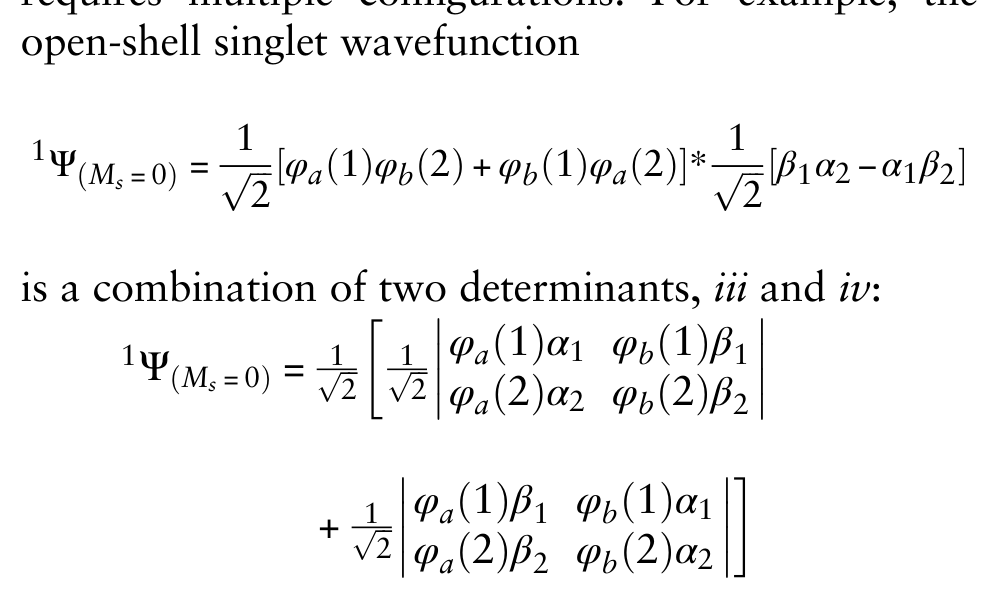
\includegraphics[height=0.56\textheight]{screenshots/sign_error_raw.png}
  \vskip0.1cm
  \onslide<2->{\small Line 1 (product form) \ldots\ then ``is a combination of two determinants, iii and iv:''}
  \symbolstrip{the paper writes each determinant with rows $=$ electrons 1, 2 and columns $=$ spin orbitals, exactly our $D_{\text{iii}}$ and
    $D_{\text{iv}}$; its prefactor $\tfrac1{\sqrt2}\cdot\tfrac1{\sqrt2}=\tfrac12$ matches ours}
\end{frame}

\begin{frame}{Spotted it}
  \begin{columns}[c]
    \column{0.6\textwidth}
    \centering
    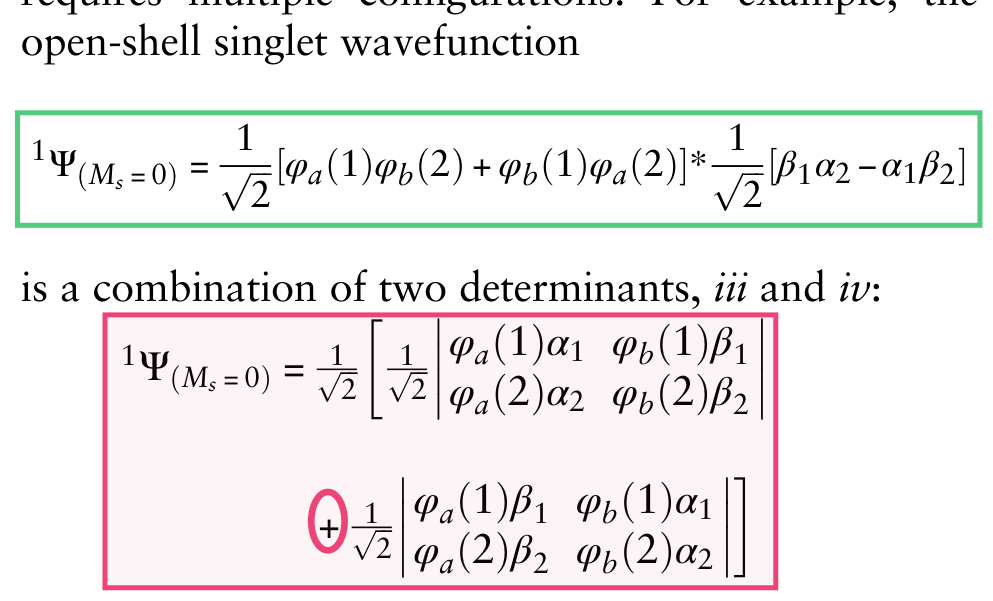
\includegraphics[width=\linewidth]{screenshots/sign_error_marked.png}
    \column{0.38\textwidth}
    \begin{itemize}
      \item<2-> \cgreen{green}: product form, symmetric space $\times$ antisymmetric spin \hfill\okpill
      \item<3-> \crose{rose}: $\tfrac12(D_{\text{iii}}\ \crose{+}\ D_{\text{iv}})$ is what we just proved to be the
            \crose{triplet} \hfill\badpill
    \end{itemize}
    \onslide<4->{
    \begin{erratum}
      should read \;$\tfrac12(D_{\text{iv}}\ \cgreen{-}\ D_{\text{iii}})$
    \end{erratum}}
  \end{columns}
  \symbolstrip{the two lines contradict each other: line 1 (green) equals $\tfrac12(D_{\text{iv}}-D_{\text{iii}})$; line 2 (rose) does not}
\end{frame}

\begin{frame}{Fluctuating multiplicity, live in print}
  \centering
  \begin{tikzpicture}
    \node[font=\noircalli\fontsize{60}{60}\selectfont,text=noirrose] (p) at (0,0) {$+$};
    \node[font=\noircalli\fontsize{60}{60}\selectfont,text=noirgreen] (m) at (5,0) {$-$};
    \draw[-{Stealth[length=7pt]},noirgold,line width=1pt] (0.9,0) -- node[above,font=\small]{one character} (4.1,0);
    \node[font=\small,text=noirrose] at (0,-1.1) {$S=1$};
    \node[font=\small,text=noirgreen] at (5,-1.1) {$S=0$};
  \end{tikzpicture}
  \vskip0.3cm
  \onslide<2->{\large The section is titled \emph{``Fluctuating ground-state multiplicity''}\ldots}
  \vskip0.2cm
  \onslide<3->{\large \ldots and between two lines the open-shell singlet \cgold{fluctuates into a triplet}.}
  \vskip0.2cm
  \onslide<4->{\small\cmuted{(It survived peer review and typesetting. Two referees with parallel spins, presumably:
    the Fermi hole kept them from ever meeting the error.)}}
\end{frame}

\begin{frame}[fragile]{Checked three ways: SymPy, $\hat S^2$, Lean}
  \begin{columns}[T]
    \column{0.49\textwidth}
    \cgold{SymPy} (T1): symbolic expansion
\begin{minted}[fontsize=\tiny]{text}
3Psi(0)  = (iii+iv)/2           : True
1Psi_OSS = (iv-iii)/2           : True
paper's (iii+iv)/2 == OSS ?     : False
\end{minted}
    \onslide<2->{\cgold{$\hat S^2$ as an operator} (T1b): the paper's matrices on a grid}
\begin{onlyenv}<2->
\begin{minted}[fontsize=\tiny]{text}
paper:   (1/2)(|iii| + |iv|)  <S^2> = +2.000000  TRIPLET
correct: (1/2)(|iv| - |iii|)  <S^2> = +0.000000  SINGLET
paper's product form (line 1) <S^2> = +0.000000  SINGLET
\end{minted}
\end{onlyenv}
    \column{0.49\textwidth}
    \onslide<3->{\cgold{Lean 4 + Mathlib} (T17): machine-checked}
\begin{onlyenv}<3->
\begin{minted}[fontsize=\tiny]{lean4}
theorem sum_is_triplet (A B ab ba : R) :
    Diii A B ab ba + Div A B ab ba
      = (A - B) * (ab + ba) := by
  unfold Diii Div; ring

theorem erratum_plus_is_not_singlet :
    ¬ (∀ A B ab ba : ℤ,
      Diii A B ab ba + Div A B ab ba
        = (A + B) * (ba - ab)) := by
  intro h
  have := h 1 0 1 0
  simp [Diii, Div] at this
\end{minted}
\end{onlyenv}
  \end{columns}
  \symbolstrip{T1b builds the two-electron wavefunctions as numerical tensors from random orthonormal orbitals and applies
    $\hat S^2=(\hat{\mathbf s}_1+\hat{\mathbf s}_2)^2$ directly: no algebra is shared with T1 \quad $\langle S^2\rangle=S(S+1)$: 2 triplet, 0 singlet}
\end{frame}

\begin{frame}{What the two-electron problem teaches}
  \begin{columns}[c]
    \column{0.5\textwidth}
    \begin{itemize}
      \item three singlets: i, ii, OSS
      \item<2-> one triplet (three $M_S$ components)
      \item<3-> triplet $M_S=\pm1$: single determinants (v, vi); $M_S=0$ needs iii$+$iv
      \item<4-> open-shell singlet: \emph{irreducibly} two determinants, for every $M_S$
    \end{itemize}
    \column{0.47\textwidth}
    \onslide<5->{
    \begin{paperclaim}
      ``their triplet state is therefore accurately described by a single reference determinant,
      however open-shell singlets require multiconfigurational (multireference) treatment.'' (p.\ 441)
    \end{paperclaim}}
    \onslide<6->{\centering\okpill\ \small conclusion right, despite the typo\par}
  \end{columns}
  \symbolstrip{single-reference: one determinant is a good starting point (the high-spin component suffices) \quad
    multireference: several determinants with comparable weights are needed from the start}
\end{frame}

% ============================================================ energies of the 2e/2o states
\section{Energies: \texorpdfstring{$J$}{J} and \texorpdfstring{$K$}{K}}

\begin{frame}{The integrals we need}
  \begin{columns}[c]
    \column{0.58\textwidth}
    {\large
    \begin{align*}
      h_{pq}&=\int\varphi_p(\mathbf r)\,\hat h\,\varphi_q(\mathbf r)\,\dd\mathbf r\\
      \uncover<2->{\eri pqrs}&\uncover<2->{=\iint\frac{\varphi_p(1)\varphi_q(1)\,\varphi_r(2)\varphi_s(2)}{r_{12}}\,\dd\mathbf r_1\dd\mathbf r_2}\\
      \uncover<3->{J_{pq}}&\uncover<3->{=\eri ppqq}\qquad \uncover<4->{K_{pq}=\eri pqpq}
    \end{align*}}
    \onslide<5->{\small chemists' notation; real orbitals $\Rightarrow$ $\eri pqrs=\eri qprs=\eri rspq=\cdots$ (8-fold)}
    \column{0.38\textwidth}
    \centering
    \begin{tikzpicture}[scale=1.0]
      \onslide<3->{
      \shade[inner color=noircyan!70,outer color=noirbg] (0,1.6) circle (0.7);
      \shade[inner color=noirrose!70,outer color=noirbg] (2.2,1.6) circle (0.7);
      \draw[noirgold,{Stealth[length=4pt]}-{Stealth[length=4pt]}] (0.5,1.6) -- (1.7,1.6);
      \node[font=\scriptsize,text=noirfg] at (1.1,2.55) {$J$: cloud $|\pa|^2$ repels cloud $|\pb|^2$};}
      \onslide<4->{
      \shade[inner color=noirviolet!80,outer color=noirbg] (1.1,-0.2) ellipse (1.1 and 0.45);
      \node[font=\scriptsize,text=noirfg,align=center] at (1.1,-1.0) {$K$: overlap density $\pa\pb$\\repels itself};}
    \end{tikzpicture}
  \end{columns}
\end{frame}

\begin{frame}{Two elementary integrals}{orthonormality does most of the work}
  \begin{assume}
    real orthonormal orbitals $\braket{\varphi_p}{\varphi_q}=\delta_{pq}$; \ $\hat h(1)$ acts only on electron 1
  \end{assume}
  {\large
  \begin{align*}
    \mel{\varphi_p(1)\varphi_q(2)}{\hat h(1)}{\varphi_r(1)\varphi_s(2)}
      &=\underbrace{\mel{\varphi_p}{\hat h}{\varphi_r}}_{h_{pr}}\ \underbrace{\braket{\varphi_q}{\varphi_s}}_{\delta_{qs}}\\
    \uncover<2->{\mel{\varphi_p(1)\varphi_q(2)}{\hat h(2)}{\varphi_r(1)\varphi_s(2)}}
      &\uncover<2->{=\delta_{pr}\,h_{qs}}\\
    \uncover<3->{\mel{\varphi_p(1)\varphi_q(2)}{r_{12}^{-1}}{\varphi_r(1)\varphi_s(2)}}
      &\uncover<3->{=\eri prqs}
  \end{align*}}
  \onslide<4->{\centering\small\cmuted{electron 1 carries $p,r$; electron 2 carries $q,s$}\par}
\end{frame}

\begin{frame}{Triplet energy, step by step (1/2)}
  $\Phi_T=\tfrac1{\sqrt2}(\ccyan A-\crose B)$, \quad $\Hop=\hat h(1)+\hat h(2)+r_{12}^{-1}$, \quad spin part normalised $\Rightarrow$ integrates to 1
  \vskip0.2cm
  \cgold{One-electron part}
  {\large
  \begin{align*}
    \mel{A}{\hat h(1)+\hat h(2)}{A}&=h_{aa}\cdot1+1\cdot h_{bb}=h_a+h_b\\
    \uncover<2->{\mel{B}{\hat h(1)+\hat h(2)}{B}}&\uncover<2->{=h_{bb}+h_{aa}}\\
    \uncover<3->{\mel{A}{\hat h(1)+\hat h(2)}{B}}&\uncover<3->{=h_{ab}\underbrace{\delta_{ba}}_{0}+\underbrace{\delta_{ab}}_{0}h_{ba}=0}\\
    \uncover<4->{\tfrac12\bigl[(h_a+h_b)+(h_a+h_b)-0-0\bigr]}&\uncover<4->{=\boxed{h_a+h_b}}
  \end{align*}}
\end{frame}

\begin{frame}{Triplet energy, step by step (2/2)}
  \cgold{Two-electron part}
  {\large
  \begin{align*}
    \mel{A}{r_{12}^{-1}}{A}&=\eri aabb=J_{ab} &&\cmuted{p,r=a;\ q,s=b}\\
    \uncover<2->{\mel{B}{r_{12}^{-1}}{B}}&\uncover<2->{=\eri bbaa=J_{ab}}\\
    \uncover<3->{\mel{A}{r_{12}^{-1}}{B}}&\uncover<3->{=\eri abba=K_{ab}} &&\uncover<3->{\cmuted{p=a,r=b;\ q=b,s=a}}\\
    \uncover<4->{\tfrac12\bigl[J+J-K-K\bigr]}&\uncover<4->{=J_{ab}-K_{ab}}
  \end{align*}}
  \onslide<5->{
  \begin{keyresult}
    \centering $\displaystyle E_T=h_a+h_b+J_{ab}-K_{ab}$
  \end{keyresult}}
\end{frame}

\begin{frame}{Open-shell singlet and the gap}
  $\Phi_{\OSS}=\tfrac1{\sqrt2}(\ccyan A+\crose B)$: identical steps, but the cross terms enter with $+$
  {\large
  \begin{align*}
    \uncover<2->{E_{\OSS}}&\uncover<2->{=h_a+h_b+\tfrac12\bigl[J+J\hlg<3>{+K+K}\bigr]}\\
    &\uncover<3->{=h_a+h_b+J_{ab}+K_{ab}}\\[4pt]
    \uncover<4->{E_{\OSS}-E_T}&\uncover<4->{=(J_{ab}+K_{ab})-(J_{ab}-K_{ab})=\boxed{2K_{ab}}}
  \end{align*}}
  \onslide<5->{
  \centering
  \begin{tikzpicture}[scale=1.0]
    \draw[level,noirrose] (0,0) -- (1.4,0) node[right,font=\small,text=noirrose]{$E_T=h_a+h_b+J-K$};
    \draw[level,noirblue] (0,1.2) -- (1.4,1.2) node[right,font=\small,text=noirblue]{$E_{\OSS}=h_a+h_b+J+K$};
    \draw[{Stealth[length=4pt]}-{Stealth[length=4pt]},noirgold] (0.7,0.08) -- (0.7,1.12) node[midway,left,font=\small,text=noirgold]{$2K$};
  \end{tikzpicture}\par}
\end{frame}

\begin{frame}{The closed shells and their couplings}
  \begin{columns}[T]
    \column{0.48\textwidth}
    \cgold{Diagonal}
    {\large
    \begin{align*}
      E_{\text i}&=2h_a+J_{aa}\\
      \uncover<2->{E_{\text{ii}}}&\uncover<2->{=2h_b+J_{bb}}
    \end{align*}}
    \onslide<3->{\cgold{i\,--\,ii}: one-electron terms die ($\delta_{ab}=0$)
    \[
      \mel{\pa\pa}{r_{12}^{-1}}{\pb\pb}=\eri abab=K_{ab}
    \]}
    \column{0.5\textwidth}
    \onslide<4->{\cgold{i\,--\,OSS}}
    {\small
    \begin{align*}
      \uncover<4->{\mel{\Phi_{\text i}}{\Hop}{\Phi_{\OSS}}}&\uncover<4->{=\tfrac1{\sqrt2}\bigl[\mel{\pa\pa}{\Hop}{A}+\mel{\pa\pa}{\Hop}{B}\bigr]}\\
      \uncover<5->{\mel{\pa\pa}{\hat h(1)+\hat h(2)}{A}}&\uncover<5->{=0+h_{ab}}\\
      \uncover<6->{\mel{\pa\pa}{r_{12}^{-1}}{A}}&\uncover<6->{=\eri aaab=\mel{\pa\pa}{r_{12}^{-1}}{B}}\\
      \uncover<7->{\Rightarrow}&\uncover<7->{=\sqrt2\,\bigl(h_{ab}+\eri aaab\bigr)}
    \end{align*}}
  \end{columns}
\end{frame}

\begin{frame}{The full two-electron, two-orbital Hamiltonian}
  \centering
  basis $\{\Phi_{\text i},\Phi_{\text{ii}},\Phi_{\OSS}\}$ (singlets) \quad $+$ \quad the triplet on its own
  {\large
  \[
    \mathbf H_S=\begin{pmatrix}
      2h_a+J_{aa} & K_{ab} & \sqrt2\,(h_{ab}+\eri aaab)\\
      K_{ab} & 2h_b+J_{bb} & \sqrt2\,(h_{ab}+\eri bbba)\\
      \cdot & \cdot & h_a+h_b+J_{ab}+K_{ab}
    \end{pmatrix},\qquad E_T=h_a+h_b+J_{ab}-K_{ab}
  \]}
  \onslide<2->{\small orbitals of different symmetry ($\sigma_g/\sigma_u$, a symmetric diradical's NBMOs) $\Rightarrow$
    $h_{ab}=\eri aaab=\eri bbba=0$: the OSS decouples}
  \vskip0.2cm
  \onslide<3->{
  \begin{checked}[T2: brute force]
    5 random integral sets (positive-definite kernel) $\to$ PySCF full CI: singlet and triplet roots
    reproduce these closed forms to $2\times10^{-14}\,\Eh$.
  \end{checked}}
\end{frame}

\begin{frame}{Hund's rule at frozen orbitals}
  \begin{columns}[c]
    \column{0.55\textwidth}
    \begin{paperclaim}
      Hund (1925): ``of the different multiplets resulting from different configurations of electrons in
      degenerate orbitals of an atom those with greatest multiplicity have the lowest energy''
    \end{paperclaim}
    \onslide<2->{With the \emph{same} orbitals in both states:
    \[
      E_T-E_{\OSS}=-2K_{ab}<0\quad\text{if }K_{ab}>0
    \]}
    \onslide<3->{\small\cgold{Two things to prove:} $K\ge0$ \ (next section), and whether ``same orbitals'' is legitimate (it is not).}
    \column{0.4\textwidth}
    \centering
    \begin{tikzpicture}[scale=1.3]
      \draw[level] (-0.4,0) -- (0.4,0); \draw[level] (0.8,0) -- (1.6,0);
      \elup{0}{0}\elup{1.2}{0}
      \node[font=\scriptsize,text=noirrose] at (0.6,-0.45) {lower: $J-K$};
      \draw[level] (-0.4,1.3) -- (0.4,1.3); \draw[level] (0.8,1.3) -- (1.6,1.3);
      \elup{0}{1.3}\eldn{1.2}{1.3}
      \node[font=\scriptsize,text=noirblue] at (0.6,0.85) {higher: $J+K$};
    \end{tikzpicture}
  \end{columns}
\end{frame}

% ============================================================ Fermi holes, K >= 0, J >= K
\section{Fermi holes}

\begin{frame}{Where can the two electrons be?}{the pair density}
  \begin{columns}[c]
    \column{0.5\textwidth}
    {\small $P(\mathbf r_1,\mathbf r_2)=N(N-1)\sum_{\sigma_1\sigma_2}\int|\Psi|^2\,\dd x_3\cdots\dd x_N$}\par\smallskip
    \onslide<2->{two electrons, spin integrated:}
    {\begin{align*}
      \uncover<2->{P_T}&\uncover<2->{=\bigl[\pa(1)\pb(2)-\pb(1)\pa(2)\bigr]^2}\\
      \uncover<3->{P_{\OSS}}&\uncover<3->{=\bigl[\pa(1)\pb(2)+\pb(1)\pa(2)\bigr]^2}
    \end{align*}}
    \onslide<4->{set $\mathbf r_1=\mathbf r_2=\mathbf r$:
    \[
      P_T(\mathbf r,\mathbf r)=\hlr<5->{0},\qquad P_{\OSS}(\mathbf r,\mathbf r)=4\pa^2\pb^2
    \]}
    \column{0.45\textwidth}
    \onslide<5->{
    \begin{keyresult}[Fermi hole]
      same-spin electrons are \emph{never} at the same point, exactly; no approximation beyond the form of $\Psi$
    \end{keyresult}}
    \onslide<6->{\small\cmuted{The \emph{Coulomb} hole (from $1/r_{12}$ itself) is absent here: it needs configuration mixing, i.e.\ correlation.}}
  \end{columns}
\end{frame}

\begin{frame}{Seeing the Fermi hole}{two electrons in a 1-D box, orbitals $\sin\pi x$ and $\sin2\pi x$}
  \centering
  \pgfplotsset{colormap={noirmap}{rgb255(0cm)=(0,0,0); rgb255(1cm)=(30,60,110); rgb255(2cm)=(95,212,208); rgb255(3cm)=(233,185,91); rgb255(4cm)=(255,255,255)}}
  \begin{tikzpicture}
    \begin{axis}[noirplot,name=trip,width=5.5cm,height=5.5cm,view={0}{90},colormap name=noirmap,
        xlabel={$x_1$},ylabel={$x_2$},domain=0:1,y domain=0:1,samples=46,title={\crose{triplet} $P_T(x_1,x_2)$},
        xtick={0,0.5,1},ytick={0,0.5,1},enlargelimits=false]
      \addplot3[surf,shader=interp] {4*(sin(deg(pi*x))*sin(deg(2*pi*y)) - sin(deg(2*pi*x))*sin(deg(pi*y)))^2};
      \draw[noirrose,dashed,line width=0.8pt] (axis cs:0,0) -- (axis cs:1,1);
    \end{axis}
    \onslide<2->{
    \begin{axis}[noirplot,at={(trip.east)},anchor=west,xshift=1.4cm,width=5.5cm,height=5.5cm,view={0}{90},colormap name=noirmap,
        xlabel={$x_1$},domain=0:1,y domain=0:1,samples=46,title={\cblue{singlet} $P_{\OSS}(x_1,x_2)$},
        xtick={0,0.5,1},ytick={0,0.5,1},enlargelimits=false]
      \addplot3[surf,shader=interp] {4*(sin(deg(pi*x))*sin(deg(2*pi*y)) + sin(deg(2*pi*x))*sin(deg(pi*y)))^2};
      \draw[noirmuted,dashed,line width=0.8pt] (axis cs:0,0) -- (axis cs:1,1);
    \end{axis}}
  \end{tikzpicture}
  \vskip-0.1cm
  {\small dashed line $x_1=x_2$: \crose{dark all along for the triplet}\onslide<2->{, bright for the singlet}}
\end{frame}

\begin{frame}{$K_{ab}\ge0$: a three-line proof}
  overlap density \ $\rho(\mathbf r)=\pa(\mathbf r)\pb(\mathbf r)$ \ (real) \quad$\Rightarrow$\quad
  $K_{ab}=\displaystyle\iint\frac{\rho(1)\rho(2)}{r_{12}}$
  {\large
  \begin{align*}
    \stepno{1}\ \frac1{|\mathbf r|}&=\int\frac{\dd^3k}{(2\pi)^3}\,\frac{4\pi}{k^2}\,e^{i\mathbf k\cdot\mathbf r}
      &&\cmuted{\text{Fourier form of Coulomb}}\\
    \uncover<2->{\stepno{2}\ K_{ab}}&\uncover<2->{=\int\frac{\dd^3k}{(2\pi)^3}\frac{4\pi}{k^2}
      \underbrace{\Bigl(\int\rho\,e^{i\mathbf k\cdot\mathbf r_1}\Bigr)}_{\tilde\rho(\mathbf k)^*}
      \underbrace{\Bigl(\int\rho\,e^{-i\mathbf k\cdot\mathbf r_2}\Bigr)}_{\tilde\rho(\mathbf k)}}\\
    \uncover<3->{\stepno{3}\ }&\uncover<3->{=\int\frac{\dd^3k}{(2\pi)^3}\,\frac{4\pi}{k^2}\,|\tilde\rho(\mathbf k)|^2\ \hlg<4->{\ge0}}
  \end{align*}}
  \onslide<5->{\centering\small equality iff $\pa\pb\equiv0$ \ (no common region of space) \ --- this returns as \emph{disjointness}\par}
\end{frame}

\begin{frame}{$J_{ab}\ge K_{ab}$}
  \begin{columns}[c]
    \column{0.6\textwidth}
    {\large
    \begin{align*}
      \stepno{1}\ f&=\pa(1)\pb(2)-\pb(1)\pa(2)\\
      \uncover<2->{\stepno{2}\ 0}&\uncover<2->{\le\iint\frac{f^2}{r_{12}}}\\
      &\uncover<3->{=J_{ab}+J_{ab}-K_{ab}-K_{ab}}\\
      &\uncover<4->{=2(J_{ab}-K_{ab})}
    \end{align*}}
    \onslide<5->{\[\boxed{\,J_{ab}\ge K_{ab}\ge0\,}\]}
    \column{0.36\textwidth}
    \onslide<6->{
    \begin{checked}[T3]
      all canonical RHF/6-31G orbitals of H$_2$O: $\min K_{pq}=1.1\times10^{-3}\,\Eh>0$ and $J_{pq}\ge K_{pq}$ for every pair
    \end{checked}}
    \onslide<7->{\small so $E_T=h_a+h_b+J-K$ really is the lower of the two.}
  \end{columns}
\end{frame}

% ============================================================ Hund's rule, virial theorem, less screening
\section{Hund's rule}

\begin{frame}{Two explanations of the same rule}
  \begin{paperclaim}
    ``Slater's original explanation \dots\ was therefore based upon less electron--electron Coulomb repulsion
    in the triplet state \dots\ However, it has been later shown that the electron--electron repulsion is
    actually greater in the high-spin state, and an alternative explanation --- the so-called less screening
    rule --- has been offered.'' (p.\ 442)
  \end{paperclaim}
  \vskip0.2cm
  \begin{columns}[T]
    \column{0.48\textwidth}
    \onslide<2->{
    \begin{plainpanel}
      \cgold{Slater (frozen orbitals)}\\[2pt]
      $\Delta V_{ee}=-2K<0$,\ $\Delta T=0$,\ $\Delta V_{ne}=0$\\
      \small\cmuted{triplet wins by lower repulsion}
    \end{plainpanel}}
    \column{0.48\textwidth}
    \onslide<3->{
    \begin{plainpanel}
      \cgold{Less screening (relaxed orbitals)}\\[2pt]
      $\Delta V_{ee}>0$,\ $\Delta V_{ne}\ll0$,\ $\Delta T>0$\\
      \small\cmuted{triplet wins by stronger nuclear attraction}
    \end{plainpanel}}
  \end{columns}
  \vskip0.2cm
  \onslide<4->{\centering\cgold{Which one is right? The virial theorem decides.}\par}
\end{frame}

\begin{frame}{The virial theorem by scaling (1/2)}
  \begin{assume}
    an atom (nucleus at the origin); exact eigenstate $\Psi$, or any $\Psi$ optimised with respect to scaling
  \end{assume}
  {\large
  \begin{align*}
    \stepno{1}\ \Psi_\eta(\mathbf r_1,\ldots,\mathbf r_N)&=\eta^{3N/2}\,\Psi(\eta\mathbf r_1,\ldots,\eta\mathbf r_N)
      &&\cmuted{\text{squeeze ($\eta>1$) or stretch}}\\
    \uncover<2->{\stepno{2}\ \braket{\Psi_\eta}{\Psi_\eta}}&\uncover<2->{=\eta^{3N}\!\int|\Psi(\eta\mathbf r)|^2\dd^{3N}r}
      &&\uncover<2->{\cmuted{\mathbf s=\eta\mathbf r,\ \dd^{3N}r=\eta^{-3N}\dd^{3N}s}}\\
    &\uncover<3->{=\int|\Psi(\mathbf s)|^2\dd^{3N}s=1}
  \end{align*}}
  \onslide<4->{\centering\small the scaled function is still normalised, so it is a legal trial function\par}
\end{frame}

\begin{frame}{The virial theorem by scaling (2/2)}
  {\begin{align*}
    \stepno{3}\ \ev{T}_\eta&=\eta^2\ev T &&\cmuted{\nabla_{\mathbf r}=\eta\,\nabla_{\mathbf s}}\\
    \uncover<2->{\stepno{4}\ \ev{V}_\eta}&\uncover<2->{=\eta\,\ev V} &&\uncover<2->{\cmuted{-\tfrac{Z}{r}=-\eta\tfrac{Z}{s},\ \tfrac1{r_{12}}=\eta\tfrac1{s_{12}}}}\\
    \uncover<3->{\stepno{5}\ E(\eta)}&\uncover<3->{=\eta^2\ev T+\eta\ev V}\\
    \uncover<4->{\stepno{6}\ \left.\frac{\dd E}{\dd\eta}\right|_{\eta=1}}&\uncover<4->{=2\ev T+\ev V=0} &&\uncover<4->{\cmuted{\text{stationary}}}
  \end{align*}}
  \onslide<5->{
  \begin{keyresult}
    \centering $2\ev T+\ev V=0\quad\Longrightarrow\quad E=-\ev T=\tfrac12\ev V$
  \end{keyresult}}
  \onslide<6->{\footnotesize\cmuted{Lean: \texttt{scaling\_derivative}. Molecules: zero at equilibrium geometries.}}
\end{frame}

\begin{frame}{Frozen orbitals cannot be the mechanism}
  Apply the virial theorem to \emph{both} exact states and subtract:
  {\large
  \[
    \Delta E\equiv E_T-E_S=-\Delta\ev T=\tfrac12\bigl(\Delta\ev{V_{ne}}+\Delta\ev{V_{ee}}\bigr)
  \]}
  \begin{enumerate}
    \item<2-> Slater: same orbitals $\Rightarrow$ $\Delta\ev T=0$
    \item<3-> then $\Delta E=-\Delta\ev T=0$ \ \ldots\ but Slater also says $\Delta E=-2K<0$ \ \crose{contradiction}
  \end{enumerate}
  \onslide<4->{
  \begin{keyresult}
    the frozen-orbital pair violates the virial theorem, so it cannot tell us \emph{which} energy component pays
  \end{keyresult}}
  \onslide<5->{\small\cmuted{Hongo et al.\ (2004): ``This assumption leaves the kinetic energy $T$ unchanged for different spin states,
    which cannot be correct as each eigenstate must satisfy the virial theorem.''}}
\end{frame}

\begin{frame}{Less screening, as inequalities}
  \begin{assume}
    triplet lower ($\Delta E<0$), both states virial, $\Delta V_{ee}>0$ (what the calculations show)
  \end{assume}
  {\large
  \begin{align*}
    \stepno{1}\ \Delta T&=-\Delta E>0 &&\cmuted{\text{electrons more compressed}}\\
    \uncover<2->{\stepno{2}\ \Delta V}&\uncover<2->{=2\Delta E<0}\\
    \uncover<3->{\stepno{3}\ \Delta V_{ne}}&\uncover<3->{=2\Delta E-\Delta V_{ee}<2\Delta E<0}\\
    \uncover<4->{\stepno{4}\ |\Delta V_{ne}|}&\uncover<4->{>\Delta V_{ee}}
  \end{align*}}
  \onslide<5->{\centering\small\cgold{the nucleus wins}: stronger attraction over-compensates stronger repulsion \quad\cmuted{(Lean: \texttt{less\_screening})}\par}
\end{frame}

\begin{frame}{The physical picture}
  \centering
  \begin{tikzpicture}[scale=1.05]
    \begin{scope}
      \fill[noirgold] (0,0) circle (0.12);
      \draw[noircyan!60,dashed] (0,0) circle (1.6);
      \fill[noircyan] (1.3,0.9) circle (0.08) node[above,font=\scriptsize]{$e_1$};
      \fill[noircyan] (-1.4,-0.6) circle (0.08) node[below,font=\scriptsize]{$e_2$};
      \node[font=\small,text=noirblue] at (0,-2.2) {singlet: electrons may overlap,};
      \node[font=\small,text=noirblue] at (0,-2.6) {each screens the nucleus};
    \end{scope}
    \onslide<2->{
    \begin{scope}[xshift=6.5cm]
      \fill[noirgold] (0,0) circle (0.12);
      \draw[noirrose!70,dashed] (0,0) circle (1.25);
      \shade[inner color=noirbg,outer color=noirrose!25] (0.9,0.85) circle (0.55);
      \fill[noirrose] (0.9,0.85) circle (0.08) node[above=3pt,font=\scriptsize]{$e_1$};
      \fill[noirrose] (-1.05,-0.55) circle (0.08) node[below,font=\scriptsize]{$e_2$};
      \node[font=\scriptsize,text=noirrose] at (1.95,1.4) {Fermi hole};
      \node[font=\small,text=noirrose] at (0,-2.2) {triplet: kept apart, less screening,};
      \node[font=\small,text=noirrose] at (0,-2.6) {both contract towards the nucleus};
    \end{scope}}
  \end{tikzpicture}
  \vskip0.2cm
  \onslide<3->{\small contraction lowers $V_{ne}$ \ \textbullet\ raises $T$ \ \textbullet\ also raises $V_{ee}$ (closer on average)}
\end{frame}

\begin{frame}{Test 1: helium $1s2s$, solved exactly}{T4 --- $2\,^3S$ vs $2\,^1S$, 16s7p4d basis, scaled to satisfy the virial theorem}
  \begin{columns}[c]
    \column{0.55\textwidth}
    \begin{tikzpicture}
      \begin{axis}[noirplot,ybar,bar shift=0pt,width=7.2cm,height=5.6cm,bar width=16pt,ymin=-0.09,ymax=0.045,
          symbolic x coords={dE,dT,dVne,dVee},xmin=dE,xmax=dVee,enlarge x limits=0.18,xtick={dE,dT,dVne,dVee},scaled y ticks=false,
          xticklabels={$\Delta E$,$\Delta T$,$\Delta V_{ne}$,$\Delta V_{ee}$},
          ylabel={triplet $-$ singlet ($\Eh$)},yticklabel style={/pgf/number format/fixed},
          nodes near coords,every node near coord/.append style={font=\tiny,text=noirfg,/pgf/number format/fixed,/pgf/number format/precision=4},
          axis x line=bottom,axis y line=left,ymajorgrids]
        \addplot[fill=noirgold,draw=none] coordinates {(dE,-0.029347)};
        \only<2->{\addplot[fill=noircyan,draw=none] coordinates {(dT,0.029347)};}
        \only<3->{\addplot[fill=noirgreen,draw=none] coordinates {(dVne,-0.077168)};}
        \only<4->{\addplot[fill=noirrose,draw=none] coordinates {(dVee,0.018473)};}
      \end{axis}
    \end{tikzpicture}
    \column{0.42\textwidth}
    \small
    \begin{tabular}{lrr}
      \toprule & $2\,^3S$ & $2\,^1S$\\\midrule
      $E$ (ours) & $-2.175212$ & $-2.145865$\\
      $E$ (exact) & $-2.175229$ & $-2.145974$\\
      $-\ev V/\ev T$ & 2.000000 & 2.000000\\\bottomrule
    \end{tabular}
    \vskip0.3cm
    \onslide<4->{\crose{$\Delta V_{ee}>0$}: Slater's mechanism fails;\\
      \cgreen{$\Delta V_{ne}$} pays for everything.\\[3pt]
      check: $\tfrac12(-0.0772+0.0185)=-0.0293=\Delta E$}
  \end{columns}
\end{frame}

\begin{frame}{Test 2: the carbon atom (literature)}{Hongo et al., J.\ Chem.\ Phys.\ 121, 7144 (2004), Table I --- read from the arXiv full text}
  \centering
  \begin{tabular}{lrrr}
    \toprule
    $^3P-{}^1D$ ($\Eh$) & $\Delta V_{ee}$ & $\Delta V_{en}$ & $\Delta T$\\
    \midrule
    Hartree--Fock & \crose{$+0.032$} & \cgreen{$-0.145$} & $+0.057$\\
    DMC (linear estimator) & \crose{$+0.074$} & \cgreen{$-0.169$} & $+0.048$\\
    \bottomrule
  \end{tabular}
  \vskip0.4cm
  \onslide<2->{same pattern as helium: higher repulsion, much stronger attraction, higher kinetic energy}
  \vskip0.3cm
  \onslide<3->{
  \begin{keyresult}
    The review's account (less screening, $V_{ee}$ \emph{greater} in the high-spin state) is right.\hfill\okpill
  \end{keyresult}}
\end{frame}

\begin{frame}{A side claim: same-spin correlation}
  \begin{paperclaim}
    ``the absolute value of the correlation energy is approximately an order of magnitude lower for a pair of
    two same-spin electrons compared to that of opposite-spin electrons'' (p.\ 442, citing Krylov 2001)
  \end{paperclaim}
  \begin{columns}[c]
    \column{0.5\textwidth}
    \begin{tikzpicture}
      \begin{axis}[noirplot,xbar,width=6.6cm,height=3.9cm,bar width=8pt,xmin=0,xmax=0.5,
          symbolic y coords={He,C2H4,N2,H2O},ytick=data,
          yticklabels={He ($2^3S$/$1^1S$),C$_2$H$_4$ MP2,N$_2$ MP2,H$_2$O MP2},
          xlabel={same-spin / opposite-spin, per pair},
          nodes near coords,every node near coord/.append style={font=\tiny,text=noirfg},
          axis x line=bottom,axis y line=left]
        \addplot[fill=noircyan,draw=none] coordinates {(0.023,He) (0.32,C2H4) (0.43,N2) (0.43,H2O)};
        \draw[noirrose,dashed] (axis cs:0.1,He) -- (axis cs:0.1,H2O);
      \end{axis}
    \end{tikzpicture}
    \column{0.45\textwidth}
    \onslide<2->{\small dashed: ``order of magnitude'' ($0.1$)}\\[4pt]
    \onslide<3->{\small He: $0.023$, the claim holds}\\[2pt]
    \onslide<4->{\small molecular valence shells: $\approx0.3$--$0.4$ per pair (cf.\ SCS-MP2 scaling $\tfrac13$ vs $\tfrac65$)}\\[6pt]
    \onslide<5->{\warnpill\ \small true for compact two-electron systems, overstated in general (T15)}
  \end{columns}
\end{frame}

% ============================================================ static correlation: H2 and the weak-interaction limit
\section{Static correlation}

\begin{frame}{Static versus dynamic correlation}
  \begin{columns}[c]
    \column{0.5\textwidth}
    \begin{paperclaim}
      ``The weaker the interaction between the two nonbonding molecular orbitals (MOs), the stronger the
      static correlation (Figure 2).'' (p.\ 442)
    \end{paperclaim}
    \onslide<2->{\small
    \cgold{dynamic}: electrons dodging each other within one configuration\\[2pt]
    \cgold{static}: several configurations of comparable weight}
    \column{0.47\textwidth}
    \centering
    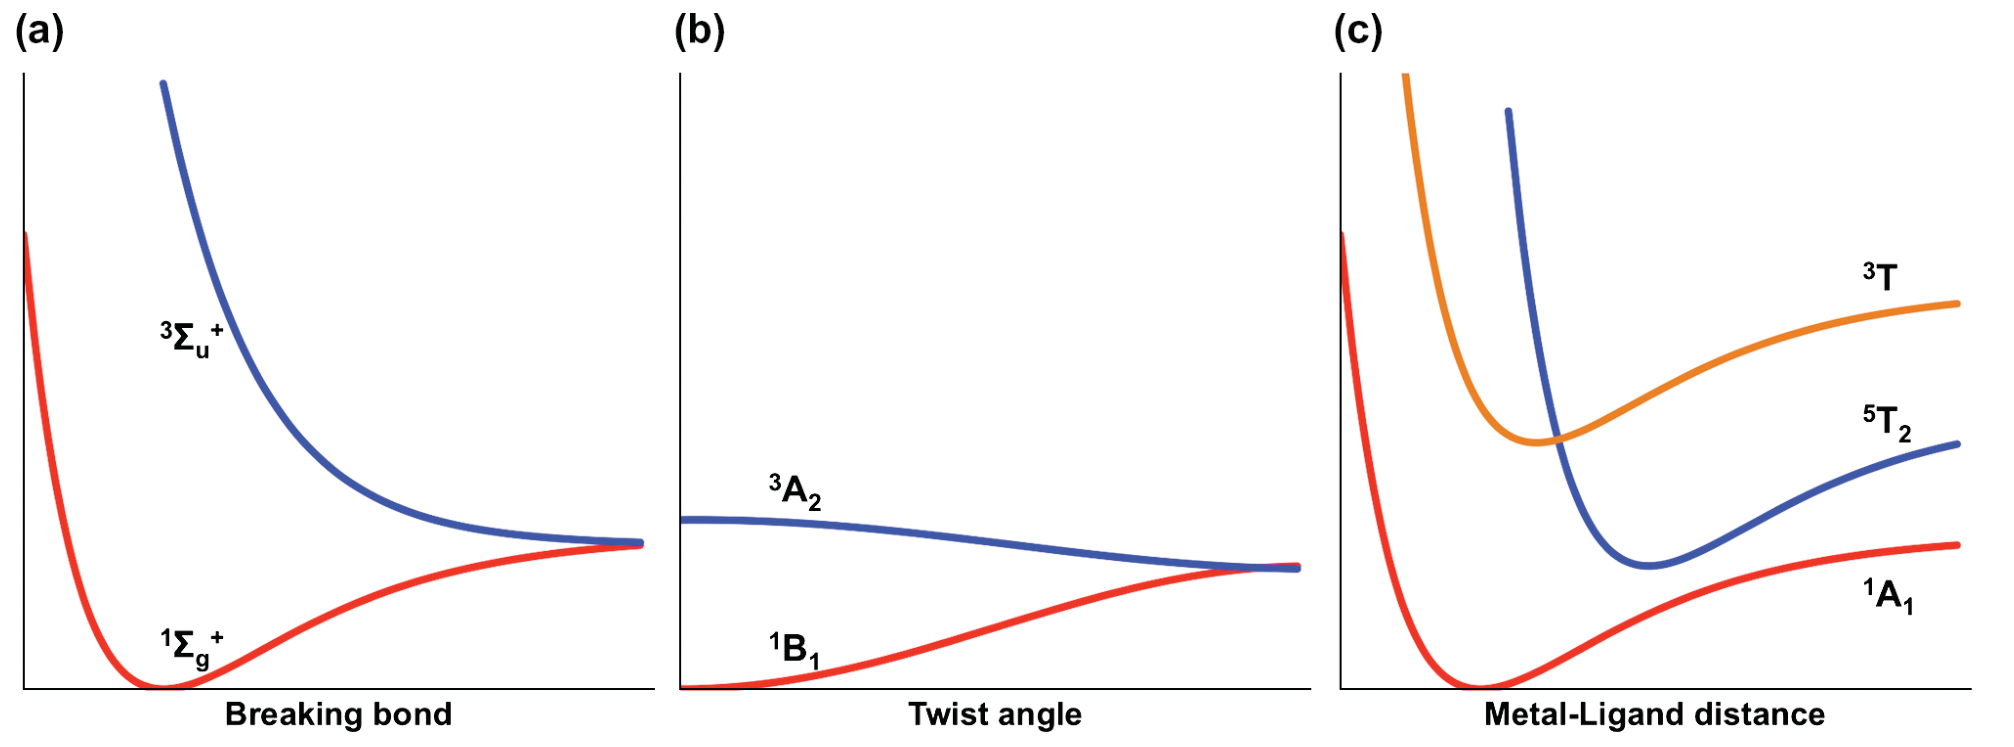
\includegraphics[width=\linewidth]{fig02_state_energies_H2_ethylene_TM.png}
    \vskip0.1cm
    {\scriptsize\cmuted{Fig.\ 2: (a) H$_2$ bond breaking (b) ethylene twist (c) metal--ligand distance}}
  \end{columns}
  \symbolstrip{correlation energy: what a single determinant (Hartree--Fock) misses \quad configuration: one way of filling the orbitals (one
    determinant or spin-adapted combination) \quad term symbols ($^1\Sigma_g^+$, $^3A_2$, \dots): spin multiplicity and spatial symmetry of a state}
\end{frame}

\begin{frame}{H$_2$ in a minimal basis}
  \begin{columns}[c]
    \column{0.55\textwidth}
    one $1s$ function per atom, $\chi_A,\chi_B$, overlap $S$:
    {\begin{align*}
      \sigma_g\equiv\varphi_1&=\frac{\chi_A+\chi_B}{\sqrt{2(1+S)}}\\
      \sigma_u\equiv\varphi_2&=\frac{\chi_A-\chi_B}{\sqrt{2(1-S)}}
    \end{align*}}
    \explain{$\sqrt{2(1\pm S)}$: $\braket{\chi_A\pm\chi_B}{\chi_A\pm\chi_B}=1+1\pm2S$}
    \onslide<2->{\small $\varphi_1$ even, $\varphi_2$ odd under inversion $\Rightarrow$
      $h_{12}=\eri1112=\eri2221=0$}
    \explain<2->{an integral with an odd number of $\varphi_2$'s has an odd integrand: it integrates to zero}
    \column{0.4\textwidth}
    \centering
    \begin{tikzpicture}[scale=0.95]
      \fill[noirgold] (-0.8,0) circle (0.07); \fill[noirgold] (0.8,0) circle (0.07);
      \shade[inner color=noircyan!60,outer color=noirbg] (0,1.4) ellipse (1.5 and 0.55);
      \node[font=\scriptsize,text=noircyan] at (0,2.15) {$\sigma_g$ (bonding)};
      \onslide<2->{
      \shade[inner color=noirrose!60,outer color=noirbg] (-0.95,-1.2) circle (0.5);
      \shade[inner color=noirblue!60,outer color=noirbg] (0.95,-1.2) circle (0.5);
      \draw[noirmuted,dashed] (0,-1.75) -- (0,-0.65);
      \node[font=\scriptsize,text=noirrose] at (0,-2.05) {$\sigma_u$ (antibonding, node)};}
    \end{tikzpicture}
  \end{columns}
  \symbolstrip{$\chi_A,\chi_B$: hydrogen $1s$ atomic orbitals on nuclei $A$, $B$ \quad $S=\braket{\chi_A}{\chi_B}$: their overlap \quad
    $g$/$u$: even/odd under inversion through the bond centre \quad indices 1, 2 below mean $\varphi_1,\varphi_2$}
\end{frame}

\begin{frame}{The $2\times2$ CI problem}
  the OSS ($^1\Sigma_u^+$) is alone; the two closed shells $\sigma_g^2,\sigma_u^2$ ($^1\Sigma_g^+$) mix:
  {\[
    \mathbf H=\begin{pmatrix}E_1&K_{12}\\K_{12}&E_2\end{pmatrix},\qquad E_1=2h_{11}+J_{11}\ (\text{RHF}),\quad E_2=2h_{22}+J_{22}
  \]}
  \explain{the coupling $K_{12}$ is the closed-shell/closed-shell element $\mel{\Phi_{\text i}}{\Hop}{\Phi_{\text{ii}}}$ derived in Part V}
  {\begin{align*}
    \uncover<2->{\det(\mathbf H-E\mathbf 1)}&\uncover<2->{=(E_1-E)(E_2-E)-K_{12}^2=0} &&\uncover<2->{\why{eigenvalue condition}}\\
    \uncover<3->{E^2-(E_1+E_2)E+E_1E_2-K_{12}^2}&\uncover<3->{=0} &&\uncover<3->{\why{multiply out}}\\
    \uncover<4->{E_{\text{CI}}}&\uncover<4->{=\tfrac12\Bigl[E_1+E_2-\sqrt{(E_2-E_1)^2+4K_{12}^2}\Bigr]} &&\uncover<4->{\why{lower root of the quadratic}}
  \end{align*}}
  \onslide<5->{\centering\small also: $E(^3\Sigma_u^+)=h_{11}+h_{22}+J_{12}-K_{12}$,\quad $E(^1\Sigma_u^+)=h_{11}+h_{22}+J_{12}+K_{12}$\par}
  \symbolstrip{CI: configuration interaction (diagonalise $\Hop$ among several configurations) \quad RHF: restricted Hartree--Fock, both electrons in $\sigma_g$
    \quad $^3\Sigma_u^+$, $^1\Sigma_u^+$: the triplet and open-shell singlet of $\sigma_g^1\sigma_u^1$}
\end{frame}

\begin{frame}{Pulling the atoms apart (1/2): the integrals}{assume $R\to\infty$: $S\to0$, every overlap density $\chi_A\chi_B\to0$; \ $U=\eri AAAA$, \ $V=\eri AABB\to1/R$}
  {\begin{align*}
    \varphi_1^2&=\tfrac12(\chi_A^2+\chi_B^2+\canc<2->{2\chi_A\chi_B})\to\tfrac12(\chi_A^2+\chi_B^2) &&\why{the atoms no longer overlap}\\
    \uncover<3->{\varphi_2^2}&\uncover<3->{\to\tfrac12(\chi_A^2+\chi_B^2)} &&\uncover<3->{\why{same, minus sign gone}}\\
    \uncover<4->{\varphi_1\varphi_2}&\uncover<4->{\to\tfrac12(\chi_A^2-\chi_B^2)} &&\uncover<4->{\why{$\tfrac12(\chi_A+\chi_B)(\chi_A-\chi_B)$}}\\
    \uncover<5->{J_{11}=J_{22}=J_{12}}&\uncover<5->{\to\tfrac14\bigl[U+V+V+U\bigr]=\tfrac12(U+V)} &&\uncover<5->{\why{4 cross terms of two $\tfrac12$-clouds}}\\
    \uncover<6->{K_{12}}&\uncover<6->{\to\tfrac14\bigl[U-V-V+U\bigr]=\tfrac12(U-V)} &&\uncover<6->{\why{the $\chi_B^2$ part enters with $-$}}
  \end{align*}}
  \onslide<7->{\centering\small and $h_{11}=h_{22}\to E_H-\tfrac1R$ \ (an electron on A still feels nucleus B as a point charge)\par}
  \symbolstrip{$R$: H--H distance \quad $U$: repulsion of two electrons on the \emph{same} atom \quad $V$: repulsion of electrons on \emph{different} atoms
    ($\to1/R$, two point charges) \quad $E_H$: energy of an isolated H atom}
\end{frame}

\begin{frame}{Pulling the atoms apart (2/2): the energies}
  \begin{align*}
    E_{\text{RHF}}&=2h_{11}+J_{11}+\tfrac1R=2E_H-\tfrac2R+\tfrac U2+\tfrac{V}{2}+\tfrac1R
      \uncover<2->{\overset{V=1/R}{=}2E_H+\hlr<3->{\tfrac U2}-\tfrac1{2R}}\\
    \uncover<4->{E_T}&\uncover<4->{=2h_{11}+J_{12}-K_{12}+\tfrac1R=2E_H-\tfrac2R+V+\tfrac1R\overset{V=1/R}{=}\hlg<5->{2E_H}}\\
    \uncover<6->{E_{\text{CI}}}&\uncover<6->{=E_1-K_{12}\ (E_1=E_2)=2E_H+\tfrac U2-\tfrac1{2R}-\tfrac{U-V}{2}\to\hlg<7->{2E_H}}\\
    \uncover<8->{E(^1\Sigma_u^+)}&\uncover<8->{=E_T+2K_{12}\to2E_H+U-V}
  \end{align*}
  \explain<2->{RHF keeps $U/2$ because half of $\sigma_g^2$ is H$^+$H$^-$; in CI, $E_1=E_2$ so the root is $E_1-K_{12}$, and $K_{12}=\tfrac{U-V}{2}$ cancels it}
  \onslide<9->{\centering\cgreen{RHF misses the dissociation limit by $U/2$; one extra configuration fixes it exactly.}\par}
  \symbolstrip{$2E_H$: the correct limit, two separate H atoms \quad $E_1=2h_{11}+J_{11}$, $E_2=2h_{22}+J_{22}$ become equal as $R\to\infty$}
\end{frame}

\begin{frame}{What the CI wavefunction is}
  at $R\to\infty$ the eigenvector is $c_1=-c_2=\tfrac1{\sqrt2}$ \quad\cgold{(two configurations, equal weight)}
  {\begin{align*}
    \uncover<2->{\varphi_1(1)\varphi_1(2)}&\uncover<2->{=\tfrac12\bigl[\underbrace{\chi_A\chi_B+\chi_B\chi_A}_{\text{covalent}}
      +\underbrace{\chi_A\chi_A+\chi_B\chi_B}_{\text{ionic}}\bigr]} &&\uncover<2->{\why{expand $(\chi_A+\chi_B)^2/2$}}\\
    \uncover<3->{\varphi_1\varphi_1-\varphi_2\varphi_2}&\uncover<3->{=\tfrac12\bigl[(\chi_A+\chi_B)^2-(\chi_A-\chi_B)^2\bigr]} &&\uncover<3->{\why{the CI combination}}\\
    &\uncover<4->{=\chi_A(1)\chi_B(2)+\chi_B(1)\chi_A(2)} &&\uncover<4->{\why{ionic terms cancel}}
  \end{align*}}
  \onslide<5->{\centering
  \begin{tikzpicture}
    \node[draw=noirrose,rounded corners,fill=noirpanel,inner sep=5pt,align=center,font=\small] at (0,0)
      {RHF: 50\% ionic\\ H$^+$H$^-$ at infinity costs $U/2$};
    \node[draw=noirgreen,rounded corners,fill=noirpanel,inner sep=5pt,align=center,font=\small] at (6,0)
      {CI: purely covalent\\ Heitler--London H$\cdot$ $\cdot$H};
  \end{tikzpicture}\par}
  \symbolstrip{covalent: one electron on each atom \quad ionic: both electrons on one atom (H$^-$ next to H$^+$) \quad
    $c_1,c_2$: CI coefficients of $\sigma_g^2$ and $\sigma_u^2$ (shorthand $\chi_A\chi_B\equiv\chi_A(1)\chi_B(2)$)}
\end{frame}

\begin{frame}{H$_2$ curves from our calculation}{STO-3G, PySCF; closed forms agree to $4\times10^{-16}\,\Eh$ (T5)}
  \centering
  \begin{tikzpicture}
    \begin{axis}[noirplot,width=11.5cm,height=5.2cm,xmin=0.8,xmax=8,ymin=-1.2,ymax=0.2,
        xlabel={$R$ (bohr)},ylabel={$E$ ($\Eh$)},legend pos=south east,legend columns=2,ymajorgrids]
      \addplot[noirmuted,dashed,thick] table[x=R,y=twoEH,col sep=comma]{data/h2_curves.csv};
      \addlegendentry{$2E_H$}
      \only<1->{\addplot[noirgold,very thick] table[x=R,y=RHF,col sep=comma]{data/h2_curves.csv};}
      \addlegendentry{RHF}
      \only<2->{\addplot[noircyan,very thick] table[x=R,y=CI,col sep=comma]{data/h2_curves.csv};}
      \only<2->{\addlegendentry{CI $=$ FCI ($^1\Sigma_g^+$)}}
      \only<3->{\addplot[noirrose,very thick] table[x=R,y=T,col sep=comma]{data/h2_curves.csv};}
      \only<3->{\addlegendentry{triplet $^3\Sigma_u^+$}}
      \only<4->{\addplot[noirblue,very thick] table[x=R,y=OSS,col sep=comma]{data/h2_curves.csv};}
      \only<4->{\addlegendentry{OSS $^1\Sigma_u^+$}}
    \end{axis}
  \end{tikzpicture}
  \vskip-0.1cm
  \onslide<3->{\small CI and triplet converge on $2E_H$; RHF does not (T5: still $0.362\,\Eh=K_{12}$ too high at $R=20$ bohr)}
  \symbolstrip{STO-3G: minimal Gaussian basis (one $1s$ function per H) \quad FCI: full CI, exact in this basis \quad
    bohr $=0.529$\,\AA \quad $2E_H=-0.9332\,\Eh$ in STO-3G}
\end{frame}

\begin{frame}{The general rule: orbital gap versus exchange}
  \begin{columns}[c]
    \column{0.48\textwidth}
    model: $h_a=-\tfrac\Delta2$, $h_b=+\tfrac\Delta2$, $J_{aa}=J_{bb}=J_d$, $J_{ab}=J_x$
    {\begin{align*}
      \uncover<2->{\mathbf H}&\uncover<2->{=\begin{pmatrix}J_d-\Delta&K\\K&J_d+\Delta\end{pmatrix}}\\
      \uncover<3->{E_S}&\uncover<3->{=J_d-\sqrt{\Delta^2+K^2}}\\
      \uncover<4->{\frac{c_2}{c_1}}&\uncover<4->{=\frac{\Delta-\sqrt{\Delta^2+K^2}}{K}}\\
      \uncover<5->{E_S-E_T}&\uncover<5->{=(J_d-J_x)+K-\sqrt{\Delta^2+K^2}}
    \end{align*}}
    \explain<2->{diagonal $2h+J$; $E_S$ is the lower root; $c_2/c_1$ from row 1, $(J_d-\Delta-E_S)c_1+Kc_2=0$; $E_T=J_x-K$}
    \column{0.5\textwidth}
    \onslide<4->{
    \begin{tikzpicture}
      \begin{axis}[noirplot,width=6.2cm,height=4.4cm,xmin=0,xmax=6,ymin=-1.05,ymax=0.05,
          xlabel={$\Delta/K$},ylabel={$c_2/c_1$},ymajorgrids]
        \addplot[noircyan,very thick,domain=0:6,samples=80] {x-sqrt(x^2+1)};
        \node[font=\scriptsize,text=noirrose,anchor=west] at (axis cs:0.15,-0.9) {diradical: equal weights};
        \node[font=\scriptsize,text=noirgreen,anchor=east] at (axis cs:5.9,-0.2) {closed shell};
      \end{axis}
    \end{tikzpicture}}
    \onslide<6->{\small\okpill\ weak interaction $\Rightarrow$ strong static correlation (T6)}
  \end{columns}
  \symbolstrip{Fig.\ 2b: twisting ethylene to $90^\circ$ closes the $\pi$/$\pi^*$ gap ($\Delta\to0$; standard result) \quad $\Delta=h_b-h_a$ \quad $J_d$: same-orbital repulsion, $J_x$: different-orbital
    \quad $c_2/c_1=-1$: two configurations of equal weight (a pure diradical); $\to0$: one configuration}
\end{frame}

% ============================================================ kinetic exchange
\section{Kinetic exchange}

\begin{frame}{The Hubbard picture}
  \begin{paperclaim}
    ``The kinetic exchange picture based on the Hubbard model \dots\ attributes stability of a singlet state in
    the case of orthogonal atomic orbitals (AOs) to the fact that perturbation yielding ionic configuration is
    allowed only from this state, and not from the triplet.'' (p.\ 442)
  \end{paperclaim}
  \vskip0.3cm
  \centering
  \begin{tikzpicture}[scale=1.1]
    \node[circle,draw=noirgold,fill=noirpanel,minimum size=1.0cm,font=\large] (l) at (0,0) {$l$};
    \node[circle,draw=noirgold,fill=noirpanel,minimum size=1.0cm,font=\large] (r) at (4,0) {$r$};
    \onslide<2->{\draw[{Stealth[length=5pt]}-{Stealth[length=5pt]},noircyan,line width=0.9pt] (l) -- node[above,font=\small,text=noircyan]{hopping $h_{lr}=-t$} (r);}
    \onslide<3->{\node[font=\small,text=noirrose] at (0,-0.95) {$U=\eri llll$};\node[font=\small,text=noirrose] at (4,-0.95) {$U=\eri rrrr$};}
    \onslide<4->{\node[font=\small,text=noirviolet] at (2,-0.55) {$V=\eri llrr$};}
    \onslide<5->{\node[font=\small,text=noirgreen] at (2,-1.1) {$k=\eri lrlr\ge0$};}
  \end{tikzpicture}
\end{frame}

\begin{frame}{Step 1: ionic configurations are pure singlets}
  \begin{columns}[c]
    \column{0.55\textwidth}
    \begin{enumerate}
      \item ionic: both electrons in one orbital, $l(1)l(2)$
      \item<2-> that spatial part is \cgold{symmetric}
      \item<3-> antisymmetry $\Rightarrow$ its spin part must be the \cgold{singlet} $\Theta_{0,0}$
      \item<4-> $\Hop$ is spin-free, so
            $\mel{\text{ionic}}{\Hop}{\text{triplet}}\propto\braket{\Theta_{0,0}}{\Theta_{1,M}}=0$
    \end{enumerate}
    \onslide<5->{
    \begin{keyresult}
      only the singlet can borrow from ionic configurations
    \end{keyresult}}
    \column{0.4\textwidth}
    \centering
    \begin{tikzpicture}[scale=1.2]
      \draw[level] (-0.4,0) -- (0.4,0); \draw[level] (0.9,0) -- (1.7,0);
      \elup{0}{0}\eldn{1.3}{0} \node[font=\scriptsize,text=noirmuted] at (0.65,-0.45) {covalent};
      \draw[level] (-0.4,-1.4) -- (0.4,-1.4); \draw[level] (0.9,-1.4) -- (1.7,-1.4);
      \elup{0}{-1.4}\eldn{0}{-1.4} \node[font=\scriptsize,text=noirmuted] at (0.65,-1.85) {ionic $l^2$};
      \onslide<4->{\draw[-{Stealth[length=4pt]},noircyan] (2.0,-0.1) to[bend left=40] node[right,font=\scriptsize]{$-t$} (2.0,-1.3);}
    \end{tikzpicture}
  \end{columns}
\end{frame}

\begin{frame}{Step 2: the matrix}
  insert the parameters into the $2e/2o$ Hamiltonian ($h_{ll}=h_{rr}=0$, $\eri lllr=0$):
  {\large
  \[
    E_T=V-k,\qquad
    \mathbf H_S=\begin{pmatrix}U&k&-\sqrt2t\\k&U&-\sqrt2t\\-\sqrt2t&-\sqrt2t&V+k\end{pmatrix}
    \quad(ll,\ rr,\ \text{cov})
  \]}
  \onslide<2->{\cgold{Step 3}: symmetry-adapt the ionic pair, $\Phi_{\pm}=\tfrac1{\sqrt2}(ll\pm rr)$}
  {\large
  \begin{align*}
    \uncover<3->{E(\Phi_\pm)}&\uncover<3->{=U\pm k}\\
    \uncover<4->{\mel{\Phi_\pm}{\Hop}{\text{cov}}}&\uncover<4->{=\tfrac1{\sqrt2}\bigl(-\sqrt2t\mp\sqrt2t\bigr)=\{-2t,\ \hlr<5->{0}\}}
  \end{align*}}
  \onslide<5->{\centering\small $\Phi_-$ decouples; the ground singlet lives in $\{\text{cov},\Phi_+\}$\par}
\end{frame}

\begin{frame}{Step 4: solve and expand}
  {\large
  \begin{align*}
    \begin{pmatrix}V+k&-2t\\-2t&U+k\end{pmatrix}\ \Rightarrow\
    E_S&=\tfrac12\Bigl[U+V+2k-\sqrt{(U-V)^2+16t^2}\Bigr]\\
    \uncover<2->{E_S-E_T}&\uncover<2->{=\tfrac12(U-V)+2k-\tfrac12\sqrt{(U-V)^2+16t^2}}\\
    \uncover<3->{\cmuted{\sqrt{x^2+16t^2}=x+\tfrac{8t^2}{x}+\cdots}\quad}&\uncover<4->{=\hlg<5->{2k}\;\hlr<5->{-\;\frac{4t^2}{U-V}}+O\!\left(\tfrac{t^4}{(U-V)^3}\right)}
  \end{align*}}
  \onslide<5->{
  \begin{columns}[T]
    \column{0.48\textwidth}
    \begin{plainpanel}
      \cgreen{$+2k$}: potential exchange, favours the \cgreen{triplet}
    \end{plainpanel}
    \column{0.48\textwidth}
    \begin{plainpanel}
      \crose{$-4t^2/(U-V)$}: kinetic exchange, favours the \crose{singlet}
    \end{plainpanel}
  \end{columns}}
\end{frame}

\begin{frame}{Hubbard dimer: exact versus kinetic exchange}{$V=k=0$: $E_S=\tfrac12\bigl(U-\sqrt{U^2+16t^2}\bigr)$, \ $E_T=0$}
  \begin{columns}[c]
    \column{0.55\textwidth}
    \begin{tikzpicture}
      \begin{axis}[noirplot,width=7.2cm,height=5.2cm,xmin=0,xmax=0.5,ymin=-1.1,ymax=0.05,
          xlabel={$t/U$},ylabel={$(E_S-E_T)/U$},ymajorgrids,legend pos=south west]
        \addplot[noircyan,very thick,domain=0:0.5,samples=80] {(1-sqrt(1+16*x^2))/2};
        \addlegendentry{exact}
        \only<2->{\addplot[noirrose,very thick,dashed,domain=0:0.5,samples=80] {-4*x^2};}
        \only<2->{\addlegendentry{$-4t^2/U$}}
      \end{axis}
    \end{tikzpicture}
    \column{0.42\textwidth}
    \begin{itemize}
      \item<2-> agree for $t\ll U$ (strong correlation)
      \item<3-> spin Hamiltonian $J_{\text{AF}}\,\hat{\mathbf S}_1\!\cdot\!\hat{\mathbf S}_2$ with $J_{\text{AF}}=4t^2/U$
      \item<4-> this coupling, bond by bond, will build the \emph{topology rules}
    \end{itemize}
    \onslide<5->{\small\tick\ \cmuted{T7: symbolic + PySCF FCI ($t{=}1,U{=}6,V{=}1.5,k{=}0.2$)}}
  \end{columns}
\end{frame}

\begin{frame}{Ionic resonance reverses a spin state (Figure 6)}
  \begin{columns}[c]
    \column{0.5\textwidth}
    \centering
    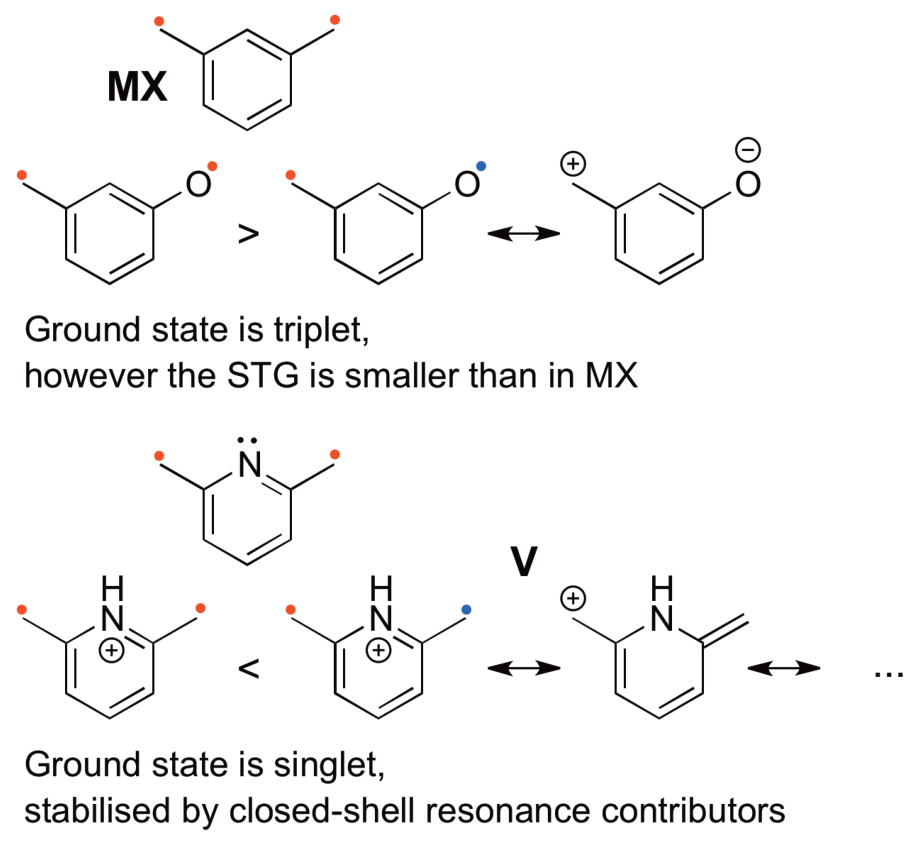
\includegraphics[width=0.95\linewidth]{fig06_ionic_resonance_spin_reversal.png}
    \column{0.47\textwidth}
    \begin{paperclaim}
      ``In the pyridinium analog of MX (V in Figure 6) this contribution exceeds the exchange and Coulomb terms,
      which formally favor the triplet state of this system with nondisjoint NBMOs.''
    \end{paperclaim}
    \onslide<2->{\small low-lying zwitterionic structures = small effective $U-V$\\
      $\Rightarrow$ $4t^2/(U-V)$ grows past $2k$ \;$\Rightarrow$\; singlet}
    \vskip0.2cm
    \onslide<3->{\small\cmuted{(a qualitative mapping: the review gives no numbers)}}
  \end{columns}
\end{frame}

\begin{frame}{Delocalised and localised: two views of one state}
  {\large
  \[
    a,b=\tfrac1{\sqrt2}(l\pm r)\quad\Rightarrow\quad
    a(1)a(2)-b(1)b(2)=l(1)r(2)+r(1)l(2)
  \]}
  \vskip0.2cm
  \begin{columns}[c]
    \column{0.48\textwidth}
    \begin{plainpanel}
      \centering\cgold{delocalised view}\\[2pt]
      two closed-shell configurations of equal weight: ``static correlation''
    \end{plainpanel}
    \column{0.48\textwidth}
    \onslide<2->{
    \begin{plainpanel}
      \centering\cgold{localised view}\\[2pt]
      one covalent configuration, no ionic part: ``no ionic character''
    \end{plainpanel}}
  \end{columns}
  \vskip0.3cm
  \onslide<3->{\centering\small same physics, different bookkeeping; the paper's two pictures are compatible\par}
\end{frame}

% ============================================================ NBMOs, disjointness
\section{NBMOs \& disjointness}

\begin{frame}{Borden \& Davidson's classification}
  \begin{columns}[c]
    \column{0.52\textwidth}
    \begin{paperclaim}
      ``If the two orbitals do not have common atoms and the probability of two electrons occupying the same space
      is nil independent of their spins, they are termed disjoint. Under such circumstances, the energy of an
      open-shell singlet can become comparable to or even lower than that of a triplet.'' (p.\ 443)
    \end{paperclaim}
    \onslide<2->{\small three things to derive: \cgold{(1)} how to find NBMOs, \cgold{(2)} when they can be disjoint,
      \cgold{(3)} why disjoint means $K\approx0$}
    \column{0.45\textwidth}
    \centering
    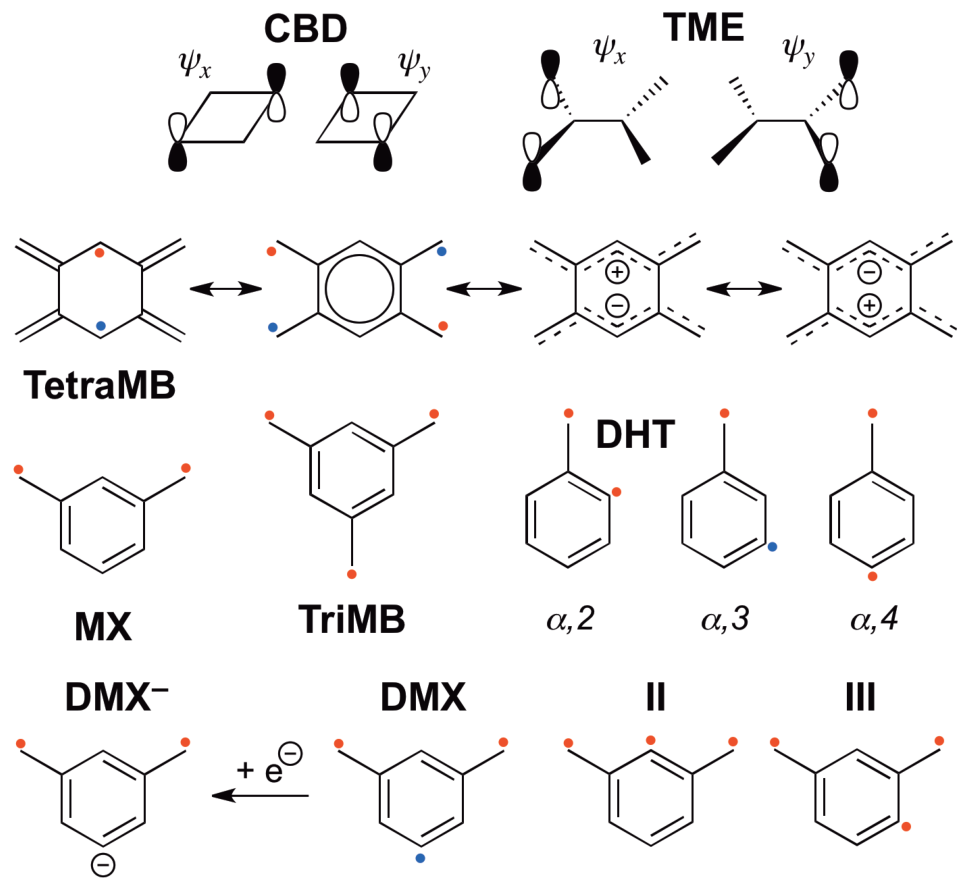
\includegraphics[width=0.95\linewidth]{fig03_high_low_spin_polyradicals.png}
    {\scriptsize\cmuted{Fig.\ 3: high- and low-spin polyradicals}}
  \end{columns}
\end{frame}

\begin{frame}{Hückel theory and the zero-sum rule}
  \begin{columns}[c]
    \column{0.55\textwidth}
    \begin{assume}[Hückel]
      one $p_\pi$ per carbon; $H_{ii}=\alpha$, $H_{ij}=\beta$ if bonded, else 0; zero overlap
    \end{assume}
    {\large
    \begin{align*}
      \mathbf H=\alpha\mathbf 1+\beta\mathbf A,\quad E&=\alpha+x\beta\ \Rightarrow\ \mathbf A\mathbf c=x\,\mathbf c\\
      \uncover<2->{\text{NBMO: }E=\alpha}&\uncover<2->{\Leftrightarrow\ \mathbf A\mathbf c=\mathbf 0}\\
      \uncover<3->{\text{row }i:\quad}&\uncover<3->{\textstyle\sum_{j\in\mathcal N(i)}c_j=0}
    \end{align*}}
    \onslide<4->{\cgold{for every atom, the NBMO coefficients of its neighbours sum to zero}}
    \column{0.4\textwidth}
    \centering
    \onslide<5->{
    \begin{tikzpicture}[scale=1.2]
      \draw[noirmuted,line width=1.2pt] (0,0) -- (1,0.6) -- (2,0);
      \foreach \x/\y/\c/\col in {0/0/0.707/noirrose,2/0/-0.707/noirblue}{
        \fill[\col,opacity=0.55] (\x,\y) circle ({0.42*abs(\c)});}
      \foreach \x/\y in {0/0,1/0.6,2/0} \fill[noirfg] (\x,\y) circle (0.05);
      \node[font=\scriptsize] at (0,-0.55) {$+\tfrac1{\sqrt2}$};
      \node[font=\scriptsize] at (1,1.0) {$0$};
      \node[font=\scriptsize] at (2,-0.55) {$-\tfrac1{\sqrt2}$};
      \node[font=\scriptsize,text=noirmuted] at (1,-1.1) {allyl NBMO: centre sees $c_1+c_3=0$};
    \end{tikzpicture}}
  \end{columns}
\end{frame}

\begin{frame}{Alternant hydrocarbons: the pairing theorem}
  star every other atom; bonds only join starred ($\mathcal A$) to unstarred ($\mathcal B$):
  {\large
  \[
    \mathbf A=\begin{pmatrix}\mathbf 0&\mathbf B\\\mathbf B^{\mathsf T}&\mathbf 0\end{pmatrix}
  \]}
  {\large
  \begin{align*}
    \uncover<2->{\mathbf A\binom{\mathbf u}{\mathbf v}=x\binom{\mathbf u}{\mathbf v}}&\uncover<2->{\ \Leftrightarrow\ \mathbf B\mathbf v=x\mathbf u,\quad\mathbf B^{\mathsf T}\mathbf u=x\mathbf v}\\
    \uncover<3->{\mathbf A\binom{\mathbf u}{-\mathbf v}}&\uncover<3->{=\binom{-\mathbf B\mathbf v}{\mathbf B^{\mathsf T}\mathbf u}=\binom{-x\mathbf u}{x\mathbf v}=\hlg<4->{-x}\binom{\mathbf u}{-\mathbf v}}
  \end{align*}}
  \onslide<4->{\centering levels come in $\pm x$ pairs, mirrored about $\alpha$ \quad\cmuted{(Lean: \texttt{pairing})}\par}
\end{frame}

\begin{frame}{How many NBMOs?}
  \begin{columns}[c]
    \column{0.56\textwidth}
    {\large
    \begin{align*}
      \operatorname{rank}\mathbf A&=2\operatorname{rank}\mathbf B\\
      \uncover<2->{}&\uncover<2->{\le2\min(n_A,n_B)}\\
      \uncover<3->{\#\text{NBMO}=N-\operatorname{rank}\mathbf A}&\uncover<3->{\ge|n_A-n_B|}
    \end{align*}}
    \onslide<4->{\small sharper (Longuet-Higgins): $\operatorname{rank}\mathbf B\le T$, the largest set of disjoint bonds
      (best Kekul\'e structure) $\Rightarrow$ \ $\#\text{NBMO}\ge N-2T$}
    \column{0.4\textwidth}
    \onslide<5->{
    \begin{erratum}[Careful: only a bound]
      square cyclobutadiene: $N=4$, $T=2$, so $N-2T=0$, yet it has \emph{two} NBMOs
    \end{erratum}}
    \onslide<5->{\centering
    \begin{tikzpicture}[scale=1.0]
      \draw[noirmuted,line width=1pt] (0,0) rectangle (1.3,1.3);
      \draw[noirgold,line width=2.2pt] (0,0) -- (1.3,0); \draw[noirgold,line width=2.2pt] (0,1.3) -- (1.3,1.3);
      \foreach \p in {(0,0),(1.3,0),(1.3,1.3),(0,1.3)} \fill[noirfg] \p circle (0.05);
      \node[font=\tiny,text=noirgold] at (0.65,-0.3) {perfect matching};
    \end{tikzpicture}\par}
    \onslide<6->{\small\cmuted{T8 caught our own wrong assumption here.}}
  \end{columns}
\end{frame}

\begin{frame}{Tetramethyleneethane: solving the zero-sum equations}
  \begin{columns}[c]
    \column{0.4\textwidth}
    \centering
    \begin{tikzpicture}[scale=0.95]
      \draw[noirmuted,line width=1pt] (-0.6,0) -- (0.6,0) (-0.6,0) -- (-1.3,1) (-0.6,0) -- (-1.3,-1) (0.6,0) -- (1.3,1) (0.6,0) -- (1.3,-1);
      \foreach \p/\l/\a in {(-0.6,0)/1/below,(0.6,0)/2/below,(-1.3,1)/3/left,(-1.3,-1)/4/left,(1.3,1)/5/right,(1.3,-1)/6/right}
        \fill[noirfg] \p circle (0.05) node[\a,font=\scriptsize]{\l};
    \end{tikzpicture}
    \column{0.56\textwidth}
    {\begin{align*}
      \text{atom 3:}\ c_1&=0 &\uncover<2->{\text{atom 5:}\ c_2}&\uncover<2->{=0}\\
      \uncover<3->{\text{atom 1:}\ c_2+c_3+c_4}&\uncover<3->{=0\Rightarrow c_4=-c_3}\\
      \uncover<4->{\text{atom 2:}\ c_1+c_5+c_6}&\uncover<4->{=0\Rightarrow c_6=-c_5}
    \end{align*}}
    \onslide<5->{\[
      \varphi_a=\tfrac1{\sqrt2}(\chi_3-\chi_4),\qquad\varphi_b=\tfrac1{\sqrt2}(\chi_5-\chi_6)
    \]}
    \onslide<6->{\centering\cgreen{no common atom: disjoint}\par}
  \end{columns}
\end{frame}

\begin{frame}{Disjoint pairs, drawn by our JavaScript}{lobe area $\propto|c_i|^2$; \crose{rose} $+$, \cblue{blue} $-$}
  \centering
  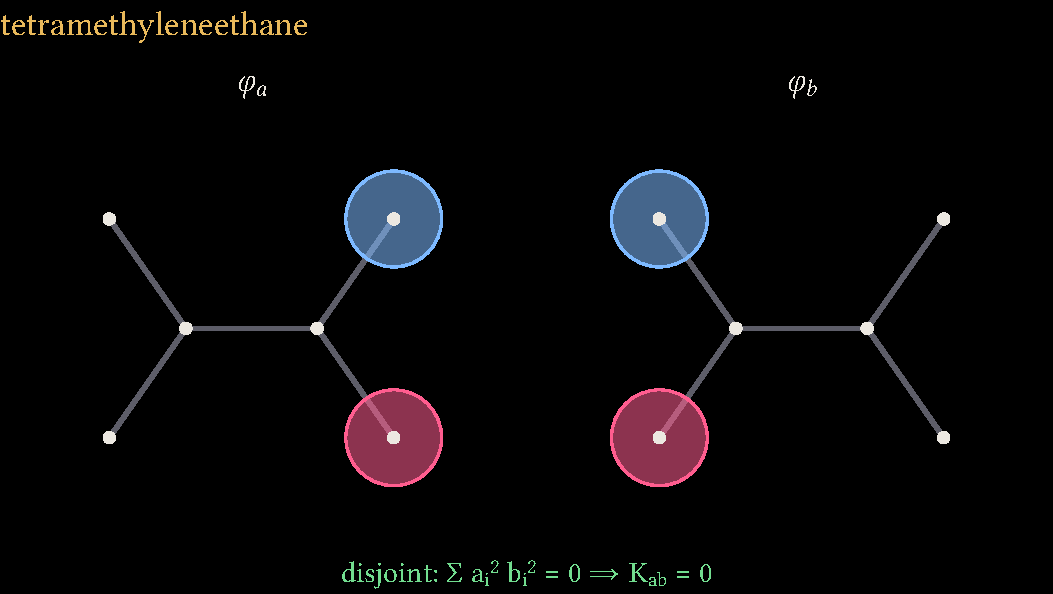
\includegraphics[width=0.53\textwidth]{diagrams/nbmo_tme.pdf}\hfill
  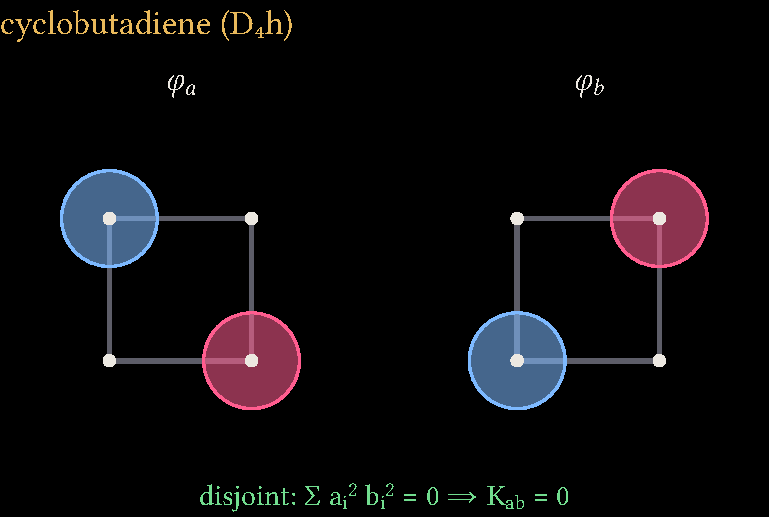
\includegraphics[width=0.44\textwidth]{diagrams/nbmo_cbd.pdf}
  \vskip0.25cm
  \onslide<2->{\small JS code: Hückel matrix $\to$ Jacobi diagonalisation $\to$ rotate the degenerate pair to minimise
    $\sum_ia_i^2b_i^2$ $\to$ SVG $\to$ PDF}
\end{frame}

\begin{frame}{Trimethylenemethane cannot be made disjoint}
  \begin{columns}[c]
    \column{0.5\textwidth}
    \begin{enumerate}
      \item zero-sum at a terminal $\Rightarrow$ $c_0=0$
      \item<2-> zero-sum at the centre $\Rightarrow$ $c_1+c_2+c_3=0$
      \item<3-> a vector in this plane with one nonzero entry cannot sum to zero: \cgold{at least 2 nonzero}
      \item<4-> two such vectors with disjoint supports need $\ge4$ terminal atoms; there are 3
    \end{enumerate}
    \onslide<5->{\centering\crose{nondisjoint, for every choice of basis}\par}
    \column{0.47\textwidth}
    \centering
    \only<5>{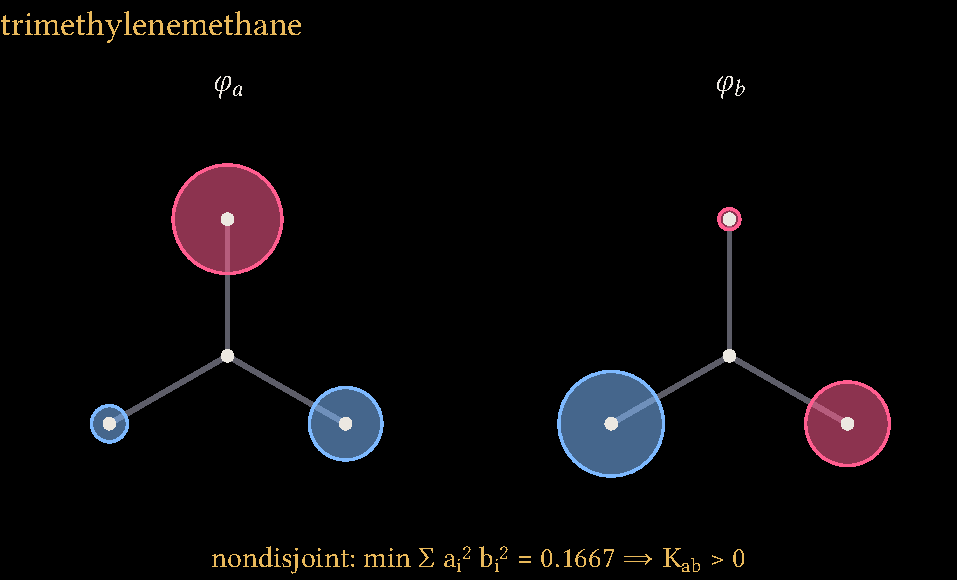
\includegraphics[width=\linewidth]{diagrams/nbmo_tmm.pdf}}
    \only<6->{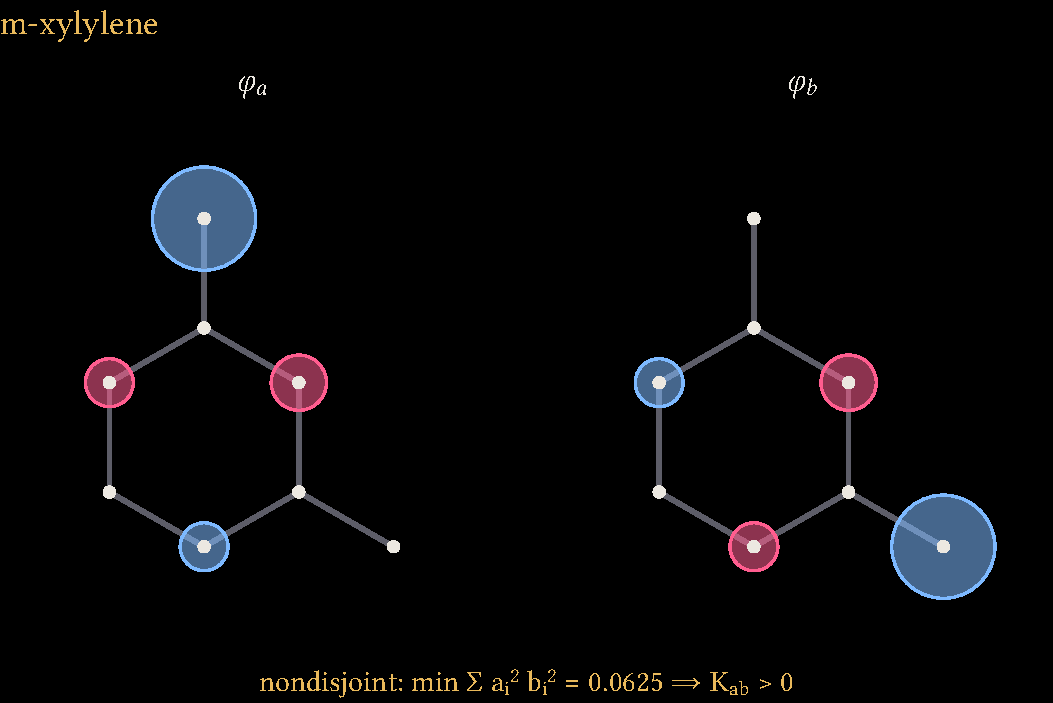
\includegraphics[width=0.9\linewidth]{diagrams/nbmo_mx.pdf}\par
      {\scriptsize\cmuted{$m$-xylylene: also nondisjoint}}}
  \end{columns}
\end{frame}

\begin{frame}{Why disjoint means $K_{ab}=0$}
  \begin{assume}[Zero differential overlap (ZDO)]
    $\eri\mu\nu\lambda\sigma=\delta_{\mu\nu}\delta_{\lambda\sigma}\,\gamma_{\mu\lambda}$, \ $\gamma$ = Coulomb repulsion between atoms $\mu,\lambda$
  \end{assume}
  {\large
  \begin{align*}
    K_{ab}=\eri abab&=\textstyle\sum_{\mu\nu\lambda\sigma}a_\mu b_\nu a_\lambda b_\sigma\,\eri\mu\nu\lambda\sigma\\
    \uncover<2->{}&\uncover<2->{=\textstyle\sum_{\mu\lambda}(a_\mu b_\mu)(a_\lambda b_\lambda)\,\gamma_{\mu\lambda}}\\
    \uncover<3->{\text{disjoint }(a_\mu b_\mu=0\ \forall\mu):\ K_{ab}}&\uncover<3->{=\hlg<3->{0}}\\
    \uncover<4->{\text{Hubbard }(\gamma_{\mu\lambda}=U\delta_{\mu\lambda}):\ K_{ab}}&\uncover<4->{=U\textstyle\sum_\mu a_\mu^2b_\mu^2}
  \end{align*}}
  \onslide<5->{\centering\small TMM: $\min\sum a^2b^2=\tfrac16$ \quad MX: $\tfrac1{16}$ \quad (Python \emph{and} JavaScript agree)\par}
\end{frame}

\begin{frame}{The test: how the gap grows with\ $U$}{T9b: exact Hubbard diagonalisation, $t=1$}
  \begin{columns}[c]
    \column{0.58\textwidth}
    \begin{tikzpicture}
      \begin{loglogaxis}[noirplot,width=7.6cm,height=5.0cm,xmin=0.04,xmax=4.5,
          xlabel={$U/t$},ylabel={$|E_T-E_S|$},ymajorgrids,
          legend style={at={(0.5,-0.3)},anchor=north,legend columns=2}]
        \addplot[noirrose,very thick,mark=*,mark size=1.2pt] table[x=U,y expr=abs(\thisrow{TMM}),col sep=comma]{data/hubbard_gap.csv};
        \addlegendentry{TMM (triplet)}
        \addplot[noirorange,very thick,mark=*,mark size=1.2pt] table[x=U,y expr=abs(\thisrow{MX}),col sep=comma]{data/hubbard_gap.csv};
        \addlegendentry{MX (triplet)}
        \only<2->{\addplot[noircyan,very thick,mark=square*,mark size=1.2pt] table[x=U,y=CBD,col sep=comma]{data/hubbard_gap.csv};}
        \only<2->{\addlegendentry{CBD (singlet)}}
        \only<2->{\addplot[noirgreen,very thick,mark=square*,mark size=1.2pt] table[x=U,y=TME,col sep=comma]{data/hubbard_gap.csv};}
        \only<2->{\addlegendentry{TME (singlet)}}
      \end{loglogaxis}
    \end{tikzpicture}
    \column{0.38\textwidth}
    \begin{itemize}
      \item nondisjoint: slope $\approx1$; \\at $U=0.05$: TMM $0.0164$ vs $2U\cdot\tfrac16=0.0167$
      \item<2-> disjoint: slope $\approx2$ (fit $1.97$, $1.95$), \\singlet below triplet
      \item<3-> first-order $K$ vanishes; something second-order picks the singlet\ldots
    \end{itemize}
  \end{columns}
\end{frame}

% ============================================================ spin polarisation, topology rules, Ovchinnikov, Lieb
\section{Spin polarisation}

\begin{frame}{Dynamic spin polarisation}
  \begin{columns}[c]
    \column{0.55\textwidth}
    \begin{paperclaim}
      ``A damped spin wave so formed generates ferromagnetic coupling between the spins separated by an odd number
      of sites, and antiferromagnetic between those separated by an even number of sites, thus yielding the
      topology rules of spin coupling.'' (p.\ 443)
    \end{paperclaim}
    \column{0.4\textwidth}
    \centering
    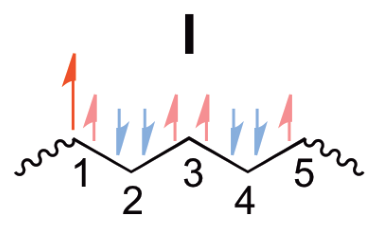
\includegraphics[width=0.72\linewidth]{scheme01_dynamic_spin_polarization.png}
    \vskip0.1cm
    {\scriptsize\cmuted{Scheme 1}}
  \end{columns}
  \onslide<2->{
  \begin{enumerate}
    \item Hückel: the unpaired electron sits in the NBMO, which is \cgold{zero on unstarred atoms}
    \item<3-> add on-site repulsion $U$: an $\uparrow$ electron pushes $\downarrow$ density onto its neighbours
    \item<4-> negative spin density appears between positive ones: \cgold{a correlation effect}
  \end{enumerate}}
  \symbolstrip{spin density $\rho_s=\rho_\uparrow-\rho_\downarrow$ on each atom \quad ferromagnetic: parallel spins; antiferromagnetic: antiparallel \quad
    ``sites'' $=$ atoms; ``separated by an odd number of sites'' $=$ odd number of atoms in between}
\end{frame}

\begin{frame}{Measured on the pentadienyl radical}{T9: exact Hubbard diagonalisation, 5 sites, 5 electrons, $S_z=\tfrac12$}
  \begin{columns}[c]
    \column{0.6\textwidth}
    \begin{tikzpicture}
      \begin{axis}[noirplot,ybar,bar shift=0pt,width=7.4cm,height=5.0cm,bar width=13pt,ymin=-0.3,ymax=0.6,
          xtick={1,2,3,4,5},xlabel={site},ylabel={spin density $\rho_s$},ymajorgrids,xmin=0.4,xmax=5.6]
        \only<1| handout:0>{\addplot[fill=noirmuted,draw=none] coordinates {(1,0.3333) (2,-0.0000) (3,0.3333) (4,-0.0000) (5,0.3333)};}
        \only<2| handout:0>{\addplot[fill=noircyan,draw=none] coordinates {(1,0.3816) (2,-0.0682) (3,0.3730) (4,-0.0682) (5,0.3816)};}
        \only<3| handout:0>{\addplot[fill=noirgold,draw=none] coordinates {(1,0.4512) (2,-0.1823) (3,0.4621) (4,-0.1823) (5,0.4512)};}
        \only<4->{\addplot[fill=noirrose,draw=none] coordinates {(1,0.4898) (2,-0.2533) (3,0.5269) (4,-0.2533) (5,0.4898)};}
      \end{axis}
    \end{tikzpicture}
    \column{0.36\textwidth}
    \only<1| handout:0>{\cmuted{$U=0$ (Hückel):}\\ unstarred sites exactly $0$}
    \only<2| handout:0>{\ccyan{$U=t$}: small negative dips}
    \only<3| handout:0>{\cgold{$U=3t$}: $-0.18$ on sites 2, 4}
    \only<4->{\crose{$U=6t$}: $-0.25$; the ``damped spin wave''}
    \vskip0.3cm
    \onslide<4->{\small total is always $1$; positive on starred, negative on unstarred atoms}
  \end{columns}
  \symbolstrip{pentadienyl: chain of 5 carbons, one unpaired electron \quad $U/t$: strength of on-site repulsion relative to hopping \quad
    $S_z=\tfrac12$: three $\uparrow$, two $\downarrow$ electrons \quad starred sites 1, 3, 5}
\end{frame}

\begin{frame}{From bonds to topology}
  \begin{columns}[c]
    \column{0.52\textwidth}
    \begin{enumerate}
      \item strong $U$: each bond carries $J_{\text{AF}}=4t^2/U$ (kinetic exchange, Part IX)
      \item<2-> bipartite graph: every bond joins $\mathcal A$ to $\mathcal B$
      \item<3-> lowest energy: $\mathcal A$ spins one way, $\mathcal B$ spins the other (Néel)
      \item<4-> same set $\Leftrightarrow$ even number of bonds $\Leftrightarrow$ odd number of atoms in between
    \end{enumerate}
    \onslide<5->{\cgold{same set: parallel; different sets: antiparallel}}
    \column{0.45\textwidth}
    \centering
    \begin{tikzpicture}[scale=0.8]
      \foreach \k in {0,...,5} \coordinate (r\k) at ({90-60*\k}:1);
      \draw[noirmuted,line width=1pt] (r0) -- (r1) -- (r2) -- (r3) -- (r4) -- (r5) -- cycle;
      \draw[noirmuted,line width=1pt] (r0) -- (90:1.9) (r2) -- (-30:1.9);
      \fill[noirrose] (90:1.9) circle (0.12); \fill[noirrose] (-30:1.9) circle (0.12);
      \node[font=\scriptsize,text=noirrose] at (0,-2.3) {meta: 3 atoms between};
      \node[font=\scriptsize,text=noirrose] at (0,-2.85) {parallel, triplet};
      \onslide<5->{
      \begin{scope}[xshift=4.2cm]
        \foreach \k in {0,...,5} \coordinate (q\k) at ({90-60*\k}:1);
        \draw[noirmuted,line width=1pt] (q0) -- (q1) -- (q2) -- (q3) -- (q4) -- (q5) -- cycle;
        \draw[noirmuted,line width=1pt] (q0) -- (90:1.9) (q3) -- (-90:1.9);
        \fill[noirrose] (90:1.9) circle (0.12); \fill[noirblue] (-90:1.9) circle (0.12);
        \node[font=\scriptsize,text=noirblue] at (0,-2.3) {para: 4 atoms between};
        \node[font=\scriptsize,text=noirblue] at (0,-2.85) {antiparallel, singlet};
      \end{scope}}
    \end{tikzpicture}
  \end{columns}
  \symbolstrip{Néel state: neighbours antiparallel everywhere \quad meta / para: $m$- / $p$-xylylene, CH$_2$ groups at ring positions 1,3 / 1,4 \quad
    a path of an even number of bonds returns to the same set}
\end{frame}

\begin{frame}{Ovchinnikov's rule, and Lieb's theorem behind it}
  \begin{columns}[c]
    \column{0.5\textwidth}
    count the Néel arrangement: $n_A$ up, $n_B$ down
    {\[
      S=\tfrac12\,|n_A-n_B|
    \]}
    \onslide<2->{\small Ovchinnikov's rule, as the review states it (p.\ 443): the most spin-alternant determinant ``is expected to have the lowest
      energy and the highest contribution''}
    \onslide<3->{
    \begin{keyresult}[Lieb, Phys.\ Rev.\ Lett.\ 62, 1201 (1989)]
      repulsive Hubbard model, bipartite graph, half filling, any $U>0$: unique ground state with
      $S=\tfrac12\bigl||\mathcal B|-|\mathcal A|\bigr|$
    \end{keyresult}}
    \column{0.46\textwidth}
    \onslide<4->{
    \small
    \begin{tabular}{lccc}
      \toprule
      T9 ($U=3t$) & $n_A/n_B$ & rule & exact\\
      \midrule
      CBD & 2/2 & 0 & \cgreen{0}\\
      TMM & 1/3 & 1 & \cgreen{1}\\
      TME & 3/3 & 0 & \cgreen{0}\\
      MX & 3/5 & 1 & \cgreen{1}\\
      TriMB & 3/6 & $\tfrac32$ & \cgreen{$\tfrac32$}\\
      TetraMB & 5/5 & 0 & \cgreen{0}\\
      $p$-xylylene & 4/4 & 0 & \cgreen{0}\\
      \bottomrule
    \end{tabular}}
    \onslide<5->{\scriptsize\crose{TriMB: the review (p.\ 444) groups it with MX as having ``triplet ground states''; three unpaired
      electrons give a \emph{quartet} ($S=\tfrac32$).}}
  \end{columns}
  \symbolstrip{$n_A,n_B$: starred / unstarred atom counts \quad half filling: one $\pi$ electron per carbon \quad
    $S=0$ singlet, $1$ triplet, $\tfrac32$ quartet \quad rule $=$ Ovchinnikov count; exact $=$ our diagonalisation}
\end{frame}

\begin{frame}{Disjoint diradicals: who picks the singlet?}
  \begin{columns}[c]
    \column{0.5\textwidth}
    \begin{paperclaim}
      ``In the singlet state of D$_{4h}$ CBD, the bonding $\pi$-electrons can partially localize on the same pair of
      atoms as the same-spin unpaired electrons; however, in the triplet state such advantageous spin polarization
      is not possible.'' (p.\ 443)
    \end{paperclaim}
    \column{0.46\textwidth}
    \begin{itemize}
      \item<2-> first order: $2K_{ab}=0$ (disjoint)
      \item<3-> second order: spin polarisation of the paired electrons, $\propto U^2$
      \item<4-> our scaling test: gap $\propto U^{1.97}$ (CBD), $U^{1.95}$ (TME), singlet lower
    \end{itemize}
    \onslide<5->{\okpill\ \small consistent with the spin-polarisation mechanism of the review's ref.\ 9 (Kollmar \& Staemmler,
      ``Violation of Hund's rule by spin polarization''; not accessed)}
  \end{columns}
  \symbolstrip{D$_{4h}$: square geometry \quad first order: energy from the exchange integral alone \quad
    second order: energy from mixing in excited (spin-polarised) configurations, scaling as $U^2$}
\end{frame}

\begin{frame}{Topology in the paper: Figure 4}
  \begin{columns}[c]
    \column{0.55\textwidth}
    \centering
    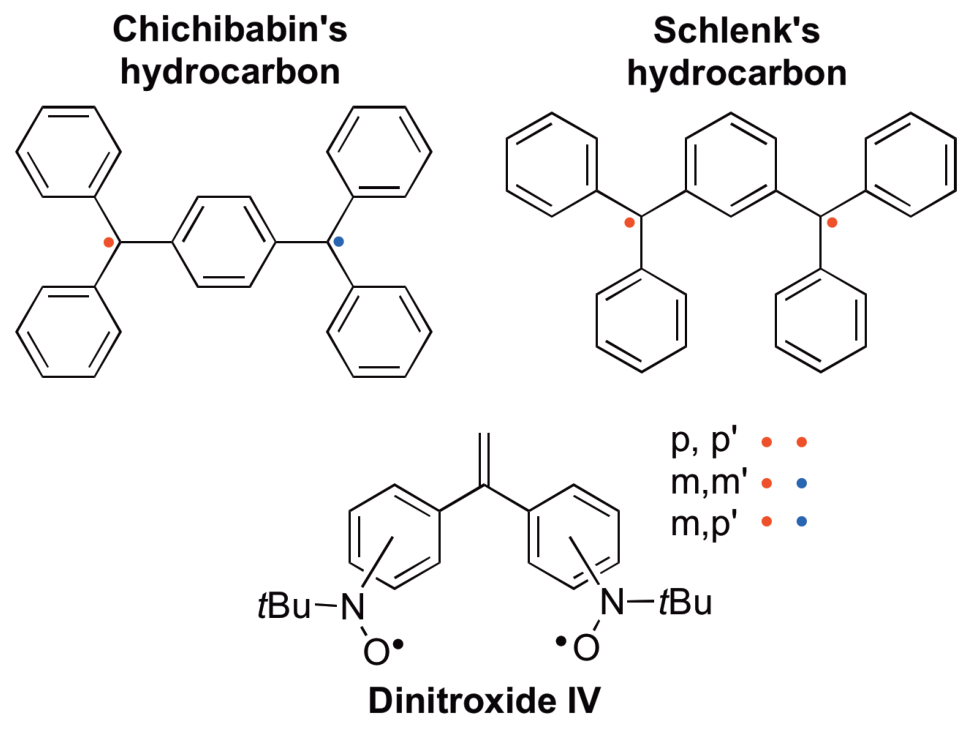
\includegraphics[width=\linewidth]{fig04_topology_driven_multiplicity.png}
    \column{0.42\textwidth}
    \begin{paperclaim}
      simple polyradicals ``can also be thought of as coupling units that sustain certain spin alignment depending on
      topology, as seen in Schlenk's and Chichibabin's hydrocarbons, or in isomers of dinitroxide IV'' (p.\ 444)
    \end{paperclaim}
    \onslide<2->{\small in Fig.\ 4, IV with $p,p'$ links: parallel spins; $m,m'$ and $m,p'$: antiparallel. Same atoms, different topology.}
  \end{columns}
  \symbolstrip{dots: \textcolor{noirrose}{rose} spin up, \textcolor{noirblue}{blue} spin down \quad $p$, $m$: para / meta attachment on each ring \quad
    Schlenk, Chichibabin: classic hydrocarbon diradicals}
\end{frame}

\begin{frame}{Tropylidene: a singlet from spin polarisation (Figure 5)}
  \begin{columns}[c]
    \column{0.5\textwidth}
    \centering
    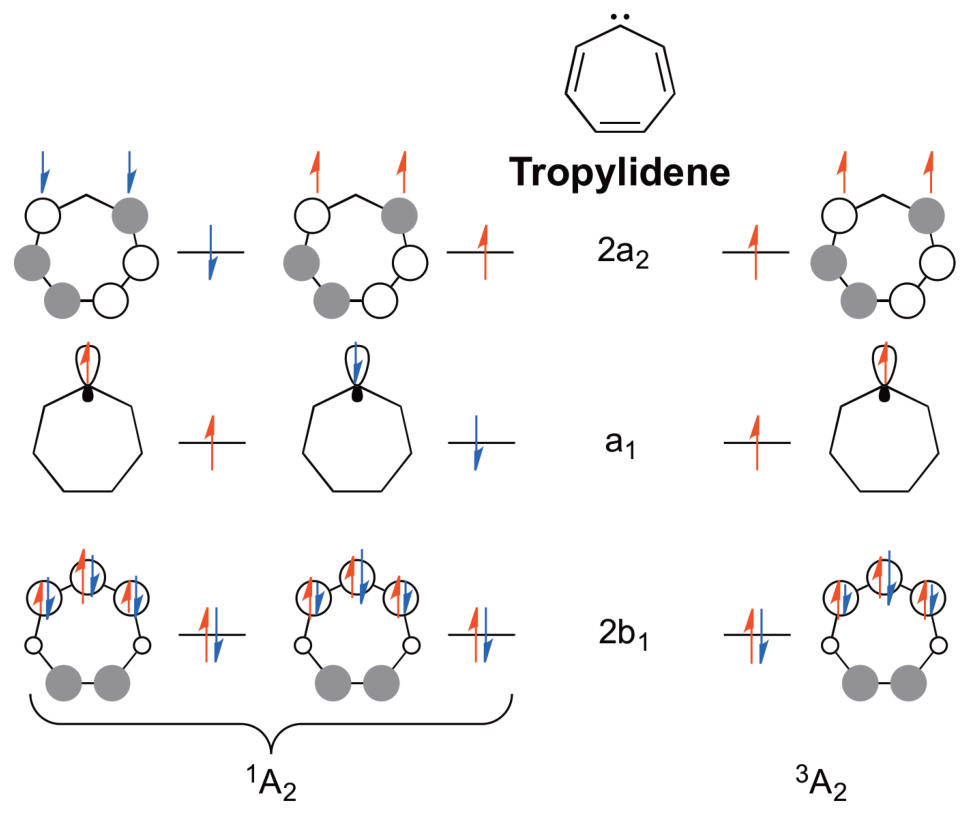
\includegraphics[width=0.92\linewidth]{fig05_tropylidene_orbitals.png}
    \column{0.47\textwidth}
    \small
    \begin{enumerate}
      \item unpaired electron in the $2a_2$ $\pi$ orbital
      \item<2-> polarises the bonding $\pi$ electrons in $2b_1$
      \item<3-> opposite spin accumulates on the carbenic carbon
      \item<4-> it couples \emph{ferromagnetically} with the electron in the orthogonal $a_1$ orbital on the same atom
      \item<5-> net result: the $^1A_2$ singlet is lower
    \end{enumerate}
    \onslide<6->{\cgold{our summary: Hund's rule obeyed locally, violated globally.}}
  \end{columns}
  \symbolstrip{tropylidene: cycloheptatrienylidene, a carbene in a 7-ring \quad $2a_2$, $2b_1$, $a_1$: orbital symmetry labels ($a_1$ in-plane, the others $\pi$) \quad
    $^1A_2$ / $^3A_2$: singlet / triplet states}
\end{frame}

\begin{frame}{Where the rules stop}
  \begin{columns}[c]
    \column{0.5\textwidth}
    \begin{itemize}
      \item Ovchinnikov / Lieb: \emph{alternant} $\pi$ systems, Hubbard/Heisenberg-type physics
      \item<2-> pyridinium V (Fig.\ 6): ionic resonance overturns the topology prediction
      \item<3-> $\sigma$--$\pi$ diradicals (didehydrotoluenes): ortho, para triplet; \emph{meta} open-shell singlet
    \end{itemize}
    \column{0.46\textwidth}
    \onslide<4->{
    \begin{paperclaim}
      ``Crucially, all of these rules are not the direct consequences of quantum mechanics and only mimic the dynamic
      and static correlation effects with the help of simplifying assumptions, thus inevitably having limited scope.'' (p.\ 443)
    \end{paperclaim}}
    \onslide<5->{\okpill\ \small fair: the topology rule is a theorem only of the Hubbard model (Lieb); the others are model heuristics}
  \end{columns}
  \symbolstrip{alternant: no odd-membered rings, so atoms split into two sets \quad $\sigma$--$\pi$ diradical: one unpaired electron in an in-plane
    $\sigma$ orbital, one in a $\pi$ orbital \quad didehydrotoluene: toluene with two H removed}
\end{frame}

% ============================================================ "exciting cases": switching spin states (Figs 7-9)
\section{Switching spin states}

\begin{frame}{Spin-state crossover by external stimuli (Figure 7)}
  \begin{columns}[c]
    \column{0.42\textwidth}
    \centering
    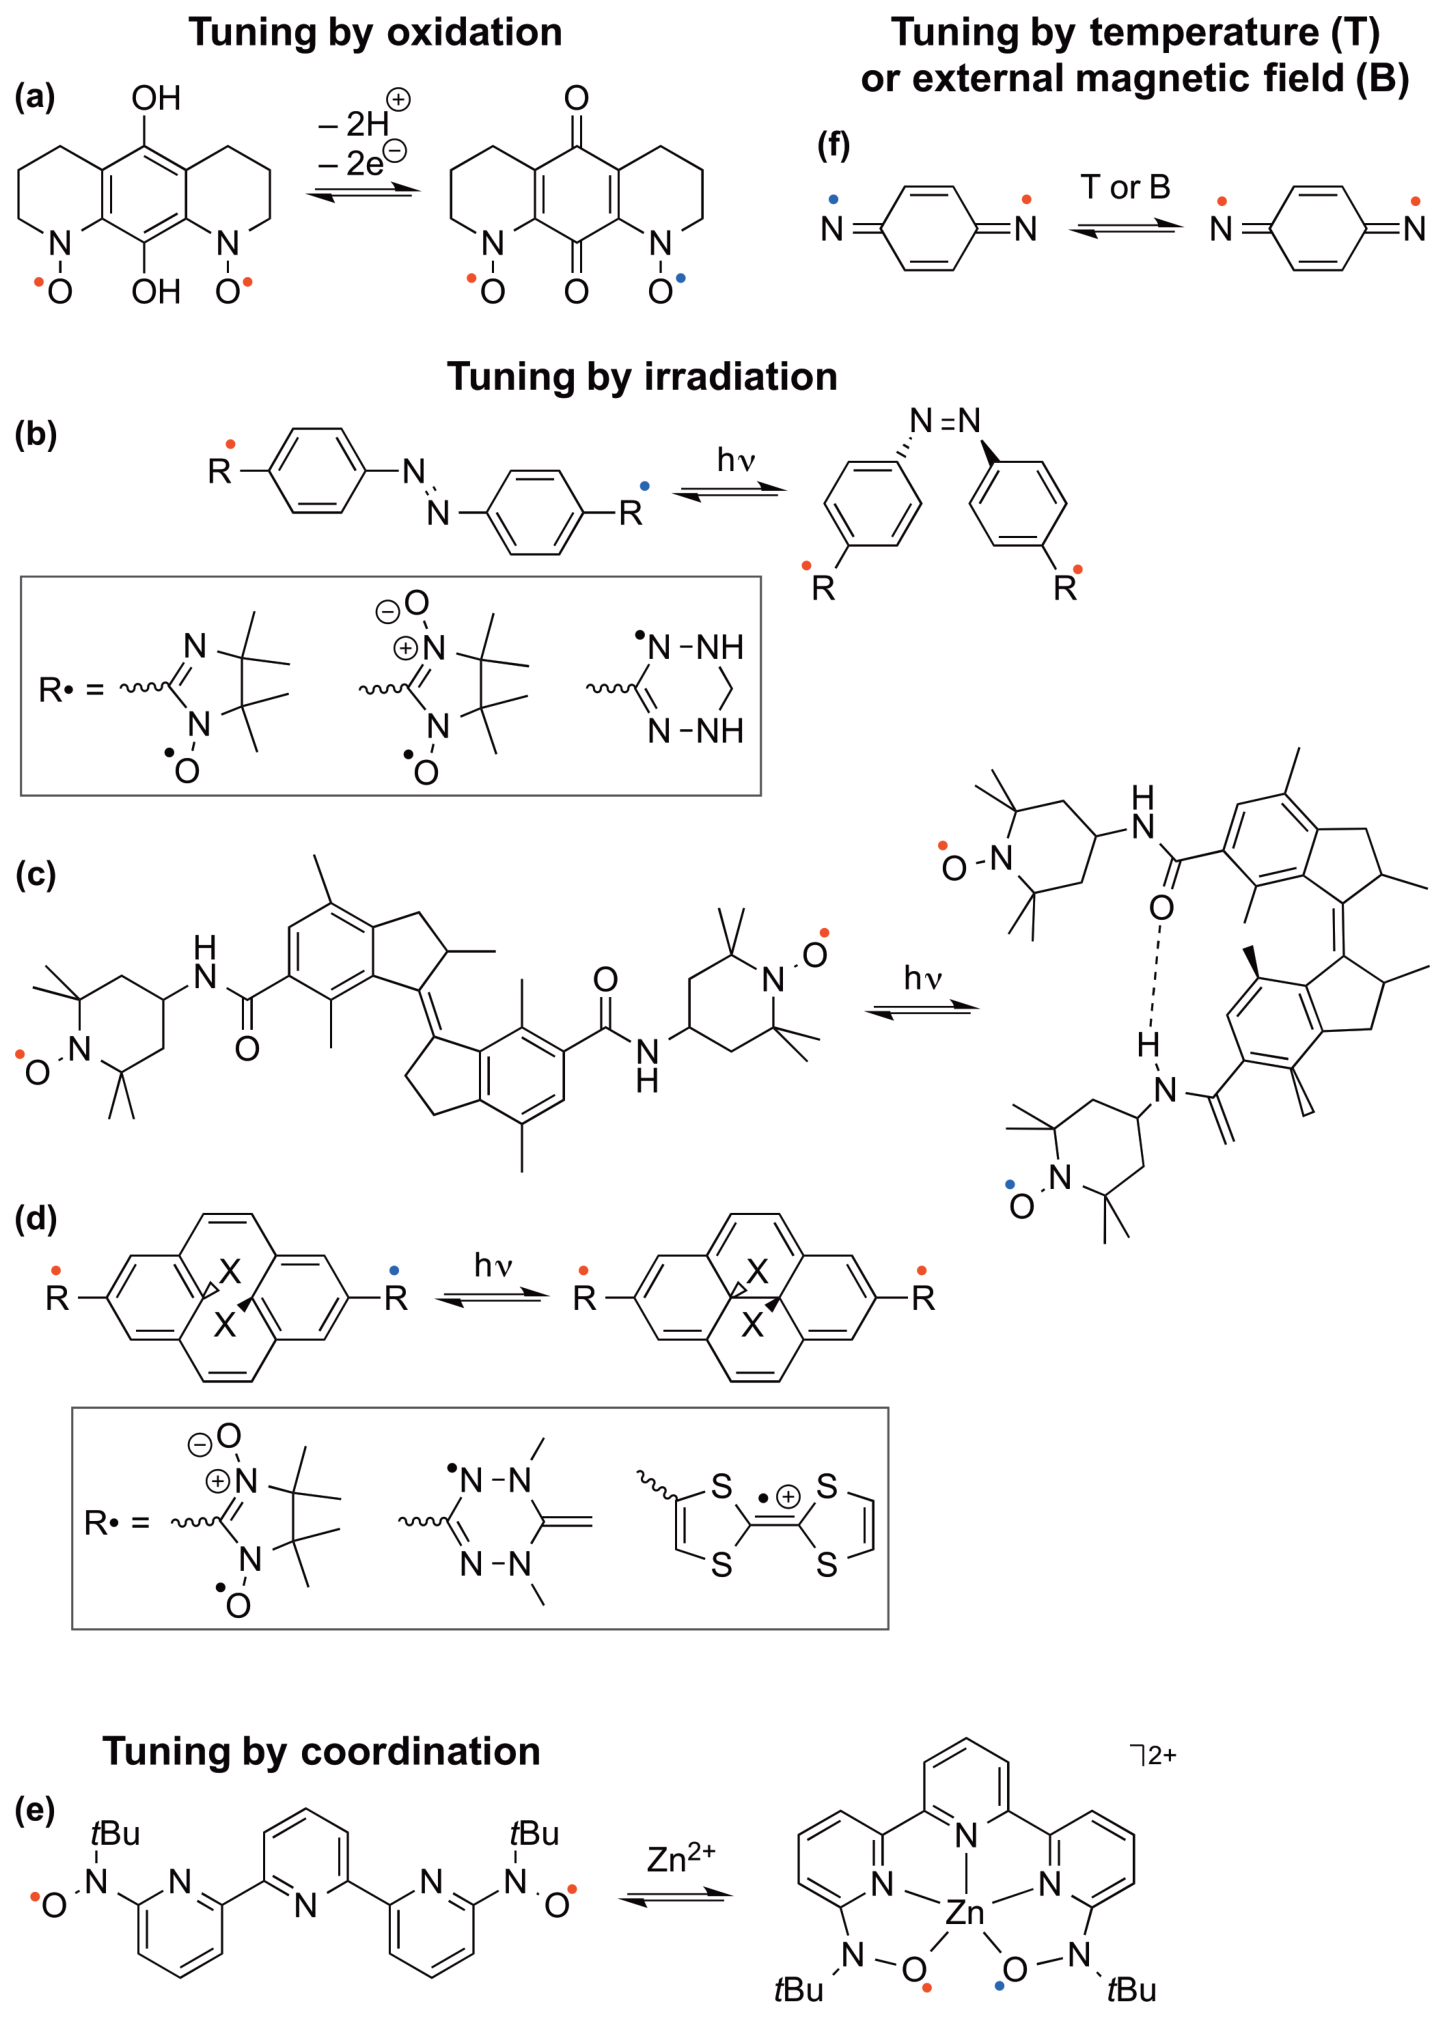
\includegraphics[height=0.74\textheight]{fig07_spin_crossover_external_stimuli.png}
    \column{0.55\textwidth}
    \footnotesize
    \begin{itemize}
      \item<1-> \cgold{(a) oxidation}: quinone coupler switches two nitroxides between ferro- and antiferromagnetic coupling
      \item<2-> \cgold{(b) light}: \emph{cis}-azobenzene loses planarity, triplet $\to$ singlet (computed)
      \item<3-> \cgold{(c) light}: \emph{trans}$\to$\emph{cis} alkene brings two TEMPO units close, H-bonded, antiferromagnetic
      \item<4-> \cgold{(d) light}: photo-induced bond formation changes the orbital topology
      \item<5-> \cgold{(e) Zn$^{2+}$}: O--Zn--O superexchange and O$\cdots$O through-space exchange favour antiferromagnetic coupling
      \item<6-> \cgold{(f) $T$ or $B$}: 1,4-phenylenedinitrene, open-shell singlet $\to$ triplet
    \end{itemize}
  \end{columns}
\end{frame}

\begin{frame}{A wording slip in (e)?}
  \begin{paperclaim}
    ``Coordination to Zn$^{2+}$ brings about O--Zn--O superexchange and O$\cdots$O through-space exchange, which favor
    antiferromagnetic coupling and override the preference for the triplet ground state, predicted on the basis of
    \emph{disjoint} NBMOs in parent dinitroxide ligand'' (p.\ 445)
  \end{paperclaim}
  \begin{columns}[T]
    \column{0.48\textwidth}
    \onslide<2->{
    \begin{plainpanel}
      review, p.\ 443: \cgold{disjoint} NBMOs make the singlet \emph{competitive};
      a \cgold{triplet} preference needs \cgold{nondisjoint} NBMOs ($K>0$)
    \end{plainpanel}}
    \column{0.48\textwidth}
    \onslide<3->{
    \begin{plainpanel}
      so ``disjoint'' here is probably meant as ``nondisjoint'', or the triplet preference has another origin
    \end{plainpanel}}
  \end{columns}
  \vskip0.1cm
  \onslide<4->{\centering\warnpill\ \small inconsistent wording; \cmuted{original (ref.\ 52) not checked}\par}
\end{frame}

\begin{frame}{Panel (f), quantitatively: temperature}
  \begin{assume}
    open-shell singlet ground state, triplet $\Delta$ above it; Boltzmann statistics; degeneracies 1 and 3
  \end{assume}
  \begin{columns}[c]
    \column{0.5\textwidth}
    {\large
    \begin{align*}
      Z&=1+3e^{-\Delta/k_BT}\\
      \uncover<2->{p_T}&\uncover<2->{=\frac{3e^{-\Delta/k_BT}}{1+3e^{-\Delta/k_BT}}}\\
      \uncover<3->{p_T(T\to\infty)}&\uncover<3->{\to\tfrac34}
    \end{align*}}
    \onslide<4->{\small ``increased temperature \dots\ promotes electrons to populate the triplet state'' \okpill}
    \column{0.46\textwidth}
    \onslide<2->{
    \begin{tikzpicture}
      \begin{axis}[noirplot,width=6.4cm,height=4.8cm,xmin=0,xmax=4,ymin=0,ymax=0.8,
          xlabel={$k_BT/\Delta$},ylabel={$p_T$},ymajorgrids]
        \addplot[noirrose,very thick,domain=0.02:4,samples=100] {3*exp(-1/x)/(1+3*exp(-1/x))};
        \draw[noirmuted,dashed] (axis cs:0,0.75) -- (axis cs:4,0.75);
      \end{axis}
    \end{tikzpicture}}
  \end{columns}
\end{frame}

\begin{frame}{Panel (f), quantitatively: magnetic field}
  \begin{columns}[c]
    \column{0.5\textwidth}
    \begin{assume}
      Zeeman term $g\mu_BBM_S$; singlet unaffected; $g\approx2$
    \end{assume}
    {\large
    \begin{align*}
      E_T(M_S)&=\Delta+g\mu_BB\,M_S,\quad M_S=0,\pm1\\
      \uncover<2->{E_T(-1)=E_S}&\uncover<2->{\ \Leftrightarrow\ B^*=\frac{\Delta}{g\mu_B}}
    \end{align*}}
    \onslide<3->{\small ``external magnetic field that splits the triplet into microstates, one of which approaches the energy of the
      ground-state singlet'' \okpill}
    \column{0.46\textwidth}
    \begin{tikzpicture}
      \begin{axis}[noirplot,width=6.4cm,height=5.2cm,xmin=0,xmax=1.5,ymin=-0.6,ymax=2.6,
          xlabel={$g\mu_BB/\Delta$},ylabel={$E/\Delta$},ymajorgrids]
        \addplot[noirblue,very thick,domain=0:1.5] {0};
        \only<1->{\addplot[noirrose,very thick,domain=0:1.5] {1+x};
                  \addplot[noirrose,very thick,domain=0:1.5] {1};
                  \addplot[noirrose,very thick,domain=0:1.5] {1-x};}
        \only<2->{\draw[noirgold,dashed] (axis cs:1,-0.6) -- (axis cs:1,2.6);}
        \node[font=\scriptsize,text=noirblue,anchor=south west] at (axis cs:0.02,0.02) {$S$};
        \node[font=\scriptsize,text=noirrose,anchor=south west] at (axis cs:0.02,1.05) {$T$};
      \end{axis}
    \end{tikzpicture}
  \end{columns}
\end{frame}

\begin{frame}{Closed shell or diradical? (Figures 8 and 9)}
  \begin{columns}[c]
    \column{0.4\textwidth}
    \centering
    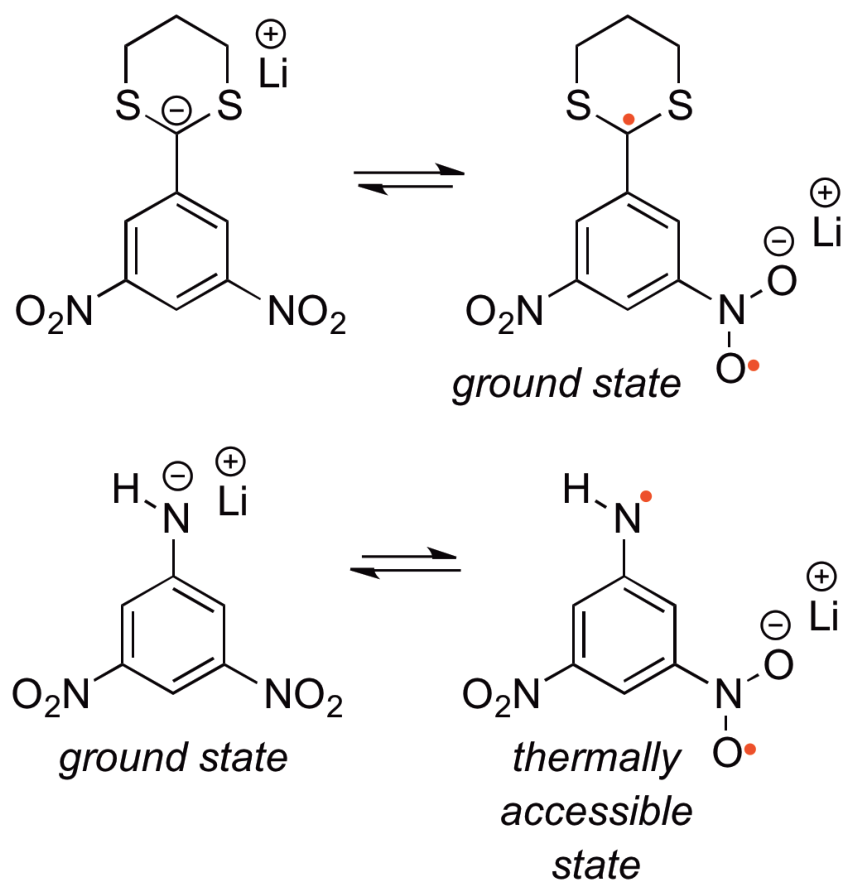
\includegraphics[width=0.9\linewidth]{fig08_borderline_triplet_closed_shell.png}
    \column{0.57\textwidth}
    \small
    \begin{itemize}
      \item \cgold{Fig.\ 8}: 1,3-dinitrophenyls with anionic substituents transfer an electron intramolecularly to give
        anionic diradicals; triplet is the ground state or only negligibly above the closed shell; cation binding to the
        nitro group stabilises the diradical
      \item<2-> \cgold{Fig.\ 9}: protonation (and oxidation) creates diradicals: donor--acceptor electron transfer after
        double protonation, a sapphyrin-derived singlet biradicaloid, a dipyrylium diradical salt, high-spin building blocks
        for polaronic ferromagnets
      \item<3-> \cgold{singlet fission}: one excited singlet shares its excitation with a neighbour; both end in a low triplet
    \end{itemize}
  \end{columns}
\end{frame}

\begin{frame}{Protonation-induced magnetisation (Figure 9)}
  \centering
  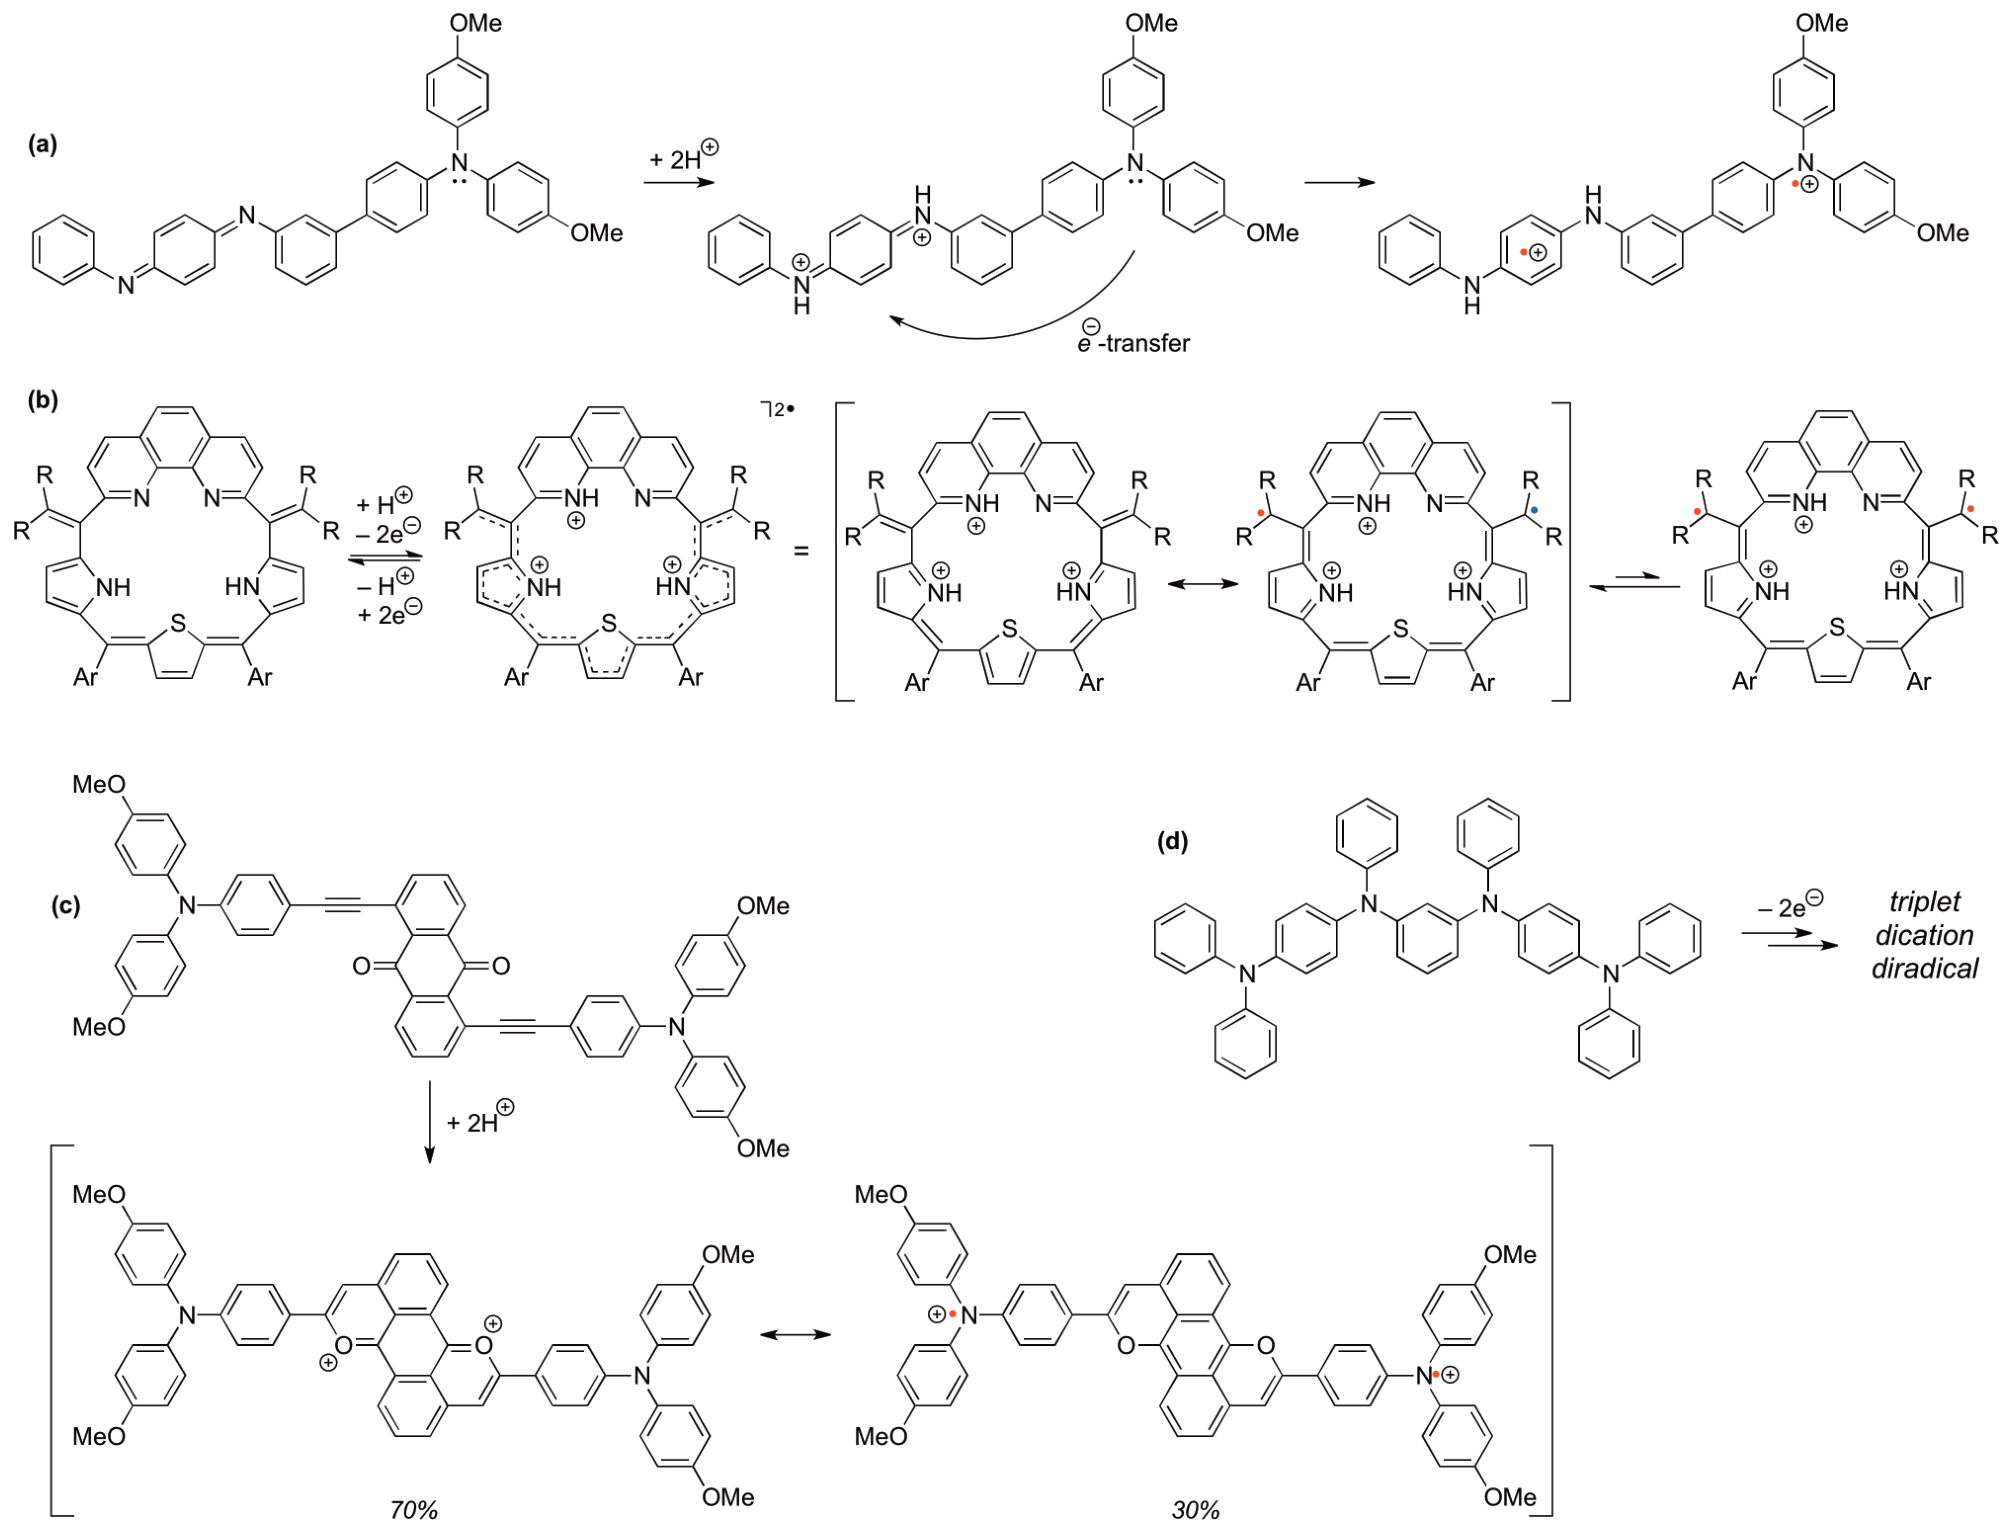
\includegraphics[height=0.64\textheight]{fig09_protonation_induced_magnetization.png}
  \vskip0.1cm
  {\small\cmuted{descriptive part of the review: no mathematics to derive, only claims about specific molecules (not re-checked)}}
\end{frame}

% ============================================================ Koopmans, Janak, S-T gap as HOMO difference
\section{Koopmans \& Janak}

\begin{frame}{The claim}
  \begin{paperclaim}
    ``An alternative theoretical interpretation of the Hund's multiplicity rule has been proposed on the basis of Janak
    theorem (or extended Koopmans' theorem) \dots: at the Hartree--Fock level, the singlet-triplet gap (STG) is equal to the
    difference between the energies of the triplet's and open-shell singlet's HOMOs.'' (p.\ 442--443)
  \end{paperclaim}
  \vskip0.2cm
  \onslide<2->{\centering three steps: \cgold{Koopmans' theorem} \;$\to$\; \cgold{Janak's theorem} \;$\to$\; \cgold{the gap}\par}
  \vskip0.2cm
  \onslide<3->{\centering\small\cmuted{(which difference, which sign? the review does not say; the derivation will)}\par}
\end{frame}

\begin{frame}{Koopmans' theorem}
  \begin{assume}
    single determinant of spin orbitals $\chi_i$; remove $\chi_k$ \emph{without} relaxing the others
  \end{assume}
  {\large
  \begin{align*}
    E_N&=\textstyle\sum_i\langle i|\hat h|i\rangle+\tfrac12\sum_{i,j}\bigl([ii|jj]-[ij|ji]\bigr)\\
    \uncover<2->{E_N-E_{N-1}^{(k)}}&\uncover<2->{=\langle k|\hat h|k\rangle+\tfrac12\textstyle\sum_j(\ldots)_{kj}+\tfrac12\sum_i(\ldots)_{ik}}\\
    &\uncover<3->{=\langle k|\hat h|k\rangle+\textstyle\sum_j\bigl([kk|jj]-[kj|jk]\bigr)}\uncover<3->{\ \ \cmuted{(\text{the }j=k\text{ term is }0)}}\\
    &\uncover<4->{=\varepsilon_k}
  \end{align*}}
  \onslide<5->{\centering\large $\mathrm{IP}_k=E_{N-1}^{(k)}-E_N=-\varepsilon_k$ \quad\small\cmuted{(frozen orbitals)}\par}
\end{frame}

\begin{frame}{Janak's theorem}
  \begin{assume}[Kohn--Sham with fractional occupations $n_i$]
    $E=\sum_in_i\langle\psi_i|-\tfrac12\nabla^2|\psi_i\rangle+\int v\rho+E_H[\rho]+E_{xc}[\rho]$, \quad $\rho=\sum_in_i|\psi_i|^2$
  \end{assume}
  {\large
  \begin{align*}
    \frac{\partial E}{\partial n_i}\bigg|_{\text{explicit}}&=\langle\psi_i|-\tfrac12\nabla^2+v+v_H+v_{xc}|\psi_i\rangle=\varepsilon_i\\
    \uncover<2->{\frac{\partial E}{\partial n_i}\bigg|_{\text{via }\psi_j}}&\uncover<2->{=\textstyle\sum_jn_j\varepsilon_j\,
      \partial_{n_i}\langle\psi_j|\psi_j\rangle=\hlg<3->{0}}
  \end{align*}}
  \onslide<3->{\centering $\boxed{\partial E/\partial n_i=\varepsilon_i}$ \ for any $E_{xc}$ \quad\small\cmuted{(Janak, Phys.\ Rev.\ B 18, 7165, 1978)}\par}
\end{frame}

\begin{frame}{The gap as a HOMO difference}
  define each state's ``HOMO energy'' as minus the cost of removing the $\pb$ electron, $\pa$ frozen; \ ion: $E_{\text{ion}}=h_a$
  {\large
  \begin{align*}
    \uncover<2->{\varepsilon_b^{T}}&\uncover<2->{=E_T-E_{\text{ion}}=h_b+J_{ab}-K_{ab}}\\
    \uncover<3->{\varepsilon_b^{\OSS}}&\uncover<3->{=E_{\OSS}-E_{\text{ion}}=h_b+J_{ab}+K_{ab}}\\
    \uncover<4->{E_{\OSS}-E_T}&\uncover<4->{=\varepsilon^{\OSS}_{\text{HOMO}}-\varepsilon^{T}_{\text{HOMO}}=2K_{ab}}
  \end{align*}}
  \onslide<5->{
  \begin{keyresult}
    true at frozen orbitals; the triplet's HOMO is lower (more bound, ``harder'') by $2K$.
    Like Slater's argument it has no relaxation and no dynamic correlation, as the review notes.\hfill\okpill
  \end{keyresult}}
\end{frame}

% ============================================================ the aufbau principle on trial
\section{Aufbau on trial}

\begin{frame}{The prosecution}
  \begin{paperclaim}
    ``the aufbau principle, by assuming the existence of unchanging stationary individual electronic states, violates the
    Pauli exclusion principle. Only the many-electron system as a whole possesses stationary states.'' (p.\ 448)
  \end{paperclaim}
  \vskip0.2cm
  \begin{columns}[T]
    \column{0.32\textwidth}
    \onslide<2->{\begin{plainpanel}\centering\cgold{Exhibit A}\\[2pt]\small one-electron quantum numbers are not conserved\end{plainpanel}}
    \column{0.32\textwidth}
    \onslide<3->{\begin{plainpanel}\centering\cgold{Exhibit B}\\[2pt]\small the adiabatic argument behind ``building up''\end{plainpanel}}
    \column{0.32\textwidth}
    \onslide<4->{\begin{plainpanel}\centering\cgold{Exhibit C}\\[2pt]\small the 3d/4s paradox\end{plainpanel}}
  \end{columns}
\end{frame}

\begin{frame}{Exhibit A: $[\hat l_{1z},1/r_{12}]\neq0$}
  $\hat l_{1z}=-i(x_1\partial_{y_1}-y_1\partial_{x_1})$, \quad
  $\partial_{y_1}r_{12}^{-1}=-\dfrac{y_1-y_2}{r_{12}^3}$, \quad $\partial_{x_1}r_{12}^{-1}=-\dfrac{x_1-x_2}{r_{12}^3}$
  {\large
  \begin{align*}
    \uncover<2->{\hat l_{1z}\,r_{12}^{-1}}&\uncover<2->{=-i\,\frac{-x_1(y_1-y_2)+y_1(x_1-x_2)}{r_{12}^3}}\\
    &\uncover<3->{=-i\,\frac{\canc<4->{-x_1y_1}+x_1y_2+\canc<4->{y_1x_1}-y_1x_2}{r_{12}^3}}\\
    &\uncover<5->{=-i\,\frac{x_1y_2-x_2y_1}{r_{12}^3}\ \crose{\neq0}}
  \end{align*}}
  \onslide<6->{\centering\small first-order operator: $[\hat l_{1z},V]f=(\hat l_{1z}V)f$ \quad$\Rightarrow$\quad $l_{1z}$ is not a constant of motion\par}
\end{frame}

\begin{frame}{\ldots but the total is conserved}
  {\large
  \begin{align*}
    \hat l_{2z}\,r_{12}^{-1}&=-i\,\frac{x_2y_1-x_1y_2}{r_{12}^3}\quad\cmuted{(\partial_{y_2}r_{12}^{-1}=+\tfrac{y_1-y_2}{r_{12}^3})}\\
    \uncover<2->{(\hat l_{1z}+\hat l_{2z})\,r_{12}^{-1}}&\uncover<2->{=-i\,\frac{(x_1y_2-x_2y_1)+(x_2y_1-x_1y_2)}{r_{12}^3}=\hlg<3->{0}}
  \end{align*}}
  \begin{columns}[c]
    \column{0.5\textwidth}
    \onslide<4->{
    \begin{keyresult}
      $[\Hop,\hat{\mathbf L}]=0$, \ $[\Hop,\hat S^2]=0$,\\ but $[\Hop,\hat{\mathbf l}_i]\neq0$
    \end{keyresult}}
    \column{0.46\textwidth}
    \onslide<5->{\small $\hat{\mathbf L}$ rotates both electrons together (keeps $r_{12}$);
      $\hat{\mathbf l}_1$ rotates one (changes $r_{12}$).\\ \tick\ \cmuted{T13, SymPy on an arbitrary $f$}}
  \end{columns}
\end{frame}

\begin{frame}{Exhibit B: the adiabatic theorem}
  \begin{paperclaim}
    Bohr assumed stationary states survive ``addition of an electron and a proton''; this rests on Ehrenfest's adiabatic
    principle, which ``does not apply to aperiodic systems'' (p.\ 448)
  \end{paperclaim}
  {\begin{align*}
    \uncover<2->{\Psi(t)}&\uncover<2->{=\textstyle\sum_nc_n(t)\,e^{i\theta_n(t)}\psi_n(t),\qquad\theta_n=-\int_0^tE_n\,\dd t'}\\
    \uncover<3->{\dot c_m}&\uncover<3->{=-\textstyle\sum_nc_n\braket{\psi_m}{\dot\psi_n}e^{i(\theta_n-\theta_m)},\qquad
      \braket{\psi_m}{\dot\psi_n}=\frac{\mel{\psi_m}{\dot{\Hop}}{\psi_n}}{E_n-E_m}}
  \end{align*}}
  \onslide<4->{\small slow $\dot{\Hop}$, finite gaps $\Rightarrow$ the system stays in the \emph{continuously connected} eigenstate.
    \cgold{But}: adding a particle changes the Hilbert space (no continuous path), and the conserved labels are
    $L,S$ of the \emph{whole} system, never one-electron labels.}
\end{frame}

\begin{frame}{Exhibit C: the 3d/4s paradox}
  \begin{paperclaim}
    4s lies slightly above 3d when both are populated, so 4s is ionised first; ``however, 4s orbital is also populated
    first, because it offers less repulsion with a 3d electron than that between two 3d electrons'' (p.\ 448)
  \end{paperclaim}
  \begin{assume}[Average of configuration]
    one-electron energies $h_d,h_s$; one average repulsion per pair type: $\bar J_{dd},\ \bar J_{ds},\ J_{ss}$
  \end{assume}
  {\large
  \[
    E(d^{n_d}s^{n_s})=n_dh_d+n_sh_s+\tbinom{n_d}{2}\bar J_{dd}+n_dn_s\bar J_{ds}+\tbinom{n_s}{2}J_{ss}
  \]}
\end{frame}

\begin{frame}{3d/4s: the algebra}
  {\begin{align*}
    E(d^ns^2)&=nh_d+2h_s+\tbinom n2\bar J_{dd}+2n\bar J_{ds}+J_{ss}\\
    \uncover<2->{E(d^{n+1}s)}&\uncover<2->{=(n+1)h_d+h_s+\tbinom{n+1}2\bar J_{dd}+(n+1)\bar J_{ds}}\\
    \uncover<3->{\Delta\equiv E(d^{n+1}s)-E(d^ns^2)}&\uncover<3->{=h_d-h_s+n\bar J_{dd}+(1-n)\bar J_{ds}-J_{ss}}
      \uncover<3->{\quad\cmuted{\tbinom{n+1}2-\tbinom n2=n}}\\
    \uncover<4->{\varepsilon_d=E(d^ns^2)-E(d^{n-1}s^2)}&\uncover<4->{=h_d+(n-1)\bar J_{dd}+2\bar J_{ds}}\\
    \uncover<5->{\varepsilon_s=E(d^ns^2)-E(d^ns^1)}&\uncover<5->{=h_s+n\bar J_{ds}+J_{ss}}
  \end{align*}}
  \onslide<6->{
  \begin{keyresult}
    \centering $\Delta=(\varepsilon_d-\varepsilon_s)+\bigl(\bar J_{dd}-\bar J_{ds}\bigr)$ \qquad\cmuted{(T12; Lean \texttt{three\_d\_four\_s})}
  \end{keyresult}}
\end{frame}

\begin{frame}{3d/4s: reading the identity}
  \begin{columns}[c]
    \column{0.52\textwidth}
    \begin{itemize}
      \item compact 3d, diffuse 4s $\Rightarrow$ $\bar J_{dd}\gg\bar J_{ds}$
      \item<2-> even with $\varepsilon_d<\varepsilon_s$: \ $\Delta>0$ if $\bar J_{dd}-\bar J_{ds}>\varepsilon_s-\varepsilon_d$ \\
        \cgold{$d^ns^2$ wins}: 4s ``fills first''
      \item<3-> from $d^ns^2$: Koopmans IPs $-\varepsilon_s<-\varepsilon_d$ \\ \cgold{4s leaves first}
    \end{itemize}
    \column{0.45\textwidth}
    \onslide<4->{
    \begin{tikzpicture}[scale=1.0]
      \draw[-{Stealth[length=4pt]},noirmuted] (-0.3,-0.2) -- (-0.3,2.9) node[above,font=\scriptsize]{energy};
      \draw[level,noircyan] (0,1.6) -- (1.2,1.6) node[right,font=\scriptsize]{$\varepsilon_s=-0.90$};
      \draw[level,noirgold] (0,1.0) -- (1.2,1.0) node[right,font=\scriptsize]{$\varepsilon_d=-1.50$};
      \node[font=\scriptsize,text=noirmuted,align=left,anchor=west] at (-0.2,0.2) {example ($n=2$):\\ $\bar J_{dd}=0.8$, $\bar J_{ds}=0.1$};
      \node[font=\small,text=noirgreen,anchor=west] at (-0.2,-0.55) {$\Delta=-0.6+0.7=+0.10$};
    \end{tikzpicture}}
  \end{columns}
  \vskip0.2cm
  \onslide<5->{\centering\small orbital energies belong to a \emph{configuration}: the building-up and removal orders need not agree\par}
\end{frame}

\begin{frame}{Verdict on the aufbau critique}
  \begin{columns}[T]
    \column{0.48\textwidth}
    \cgreen{right}
    \begin{itemize}
      \item one-electron quantum numbers are model labels (Exhibit A)
      \item<2-> orbital energies depend on the configuration (Exhibit C)
      \item<3-> non-aufbau orderings are real (VO(oep), quantum dots, LiF dissociation, the radicals ahead)
    \end{itemize}
    \column{0.48\textwidth}
    \onslide<4->{\crose{overstated}}
    \begin{itemize}
      \item<4-> an aufbau-filled \emph{determinant} is fully antisymmetric: within the orbital model it does not ``violate'' Pauli
      \item<5-> ``obsolescence'' of aufbau and Hund's rule: both still hold for almost all atoms
    \end{itemize}
    \onslide<6->{\warnpill}
  \end{columns}
\end{frame}

% ============================================================ quasi-closed-shell (non-aufbau) radicals
\section{Quasi-closed shells}

\begin{frame}{SOMO below HOMO (Figure 10)}
  \begin{columns}[c]
    \column{0.45\textwidth}
    \centering
    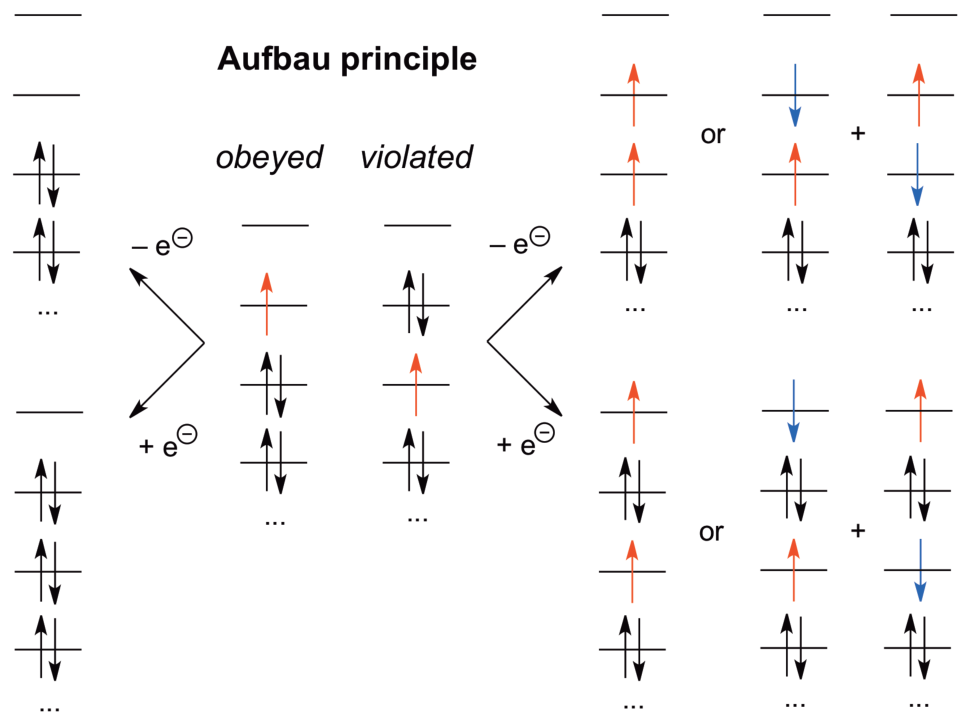
\includegraphics[width=\linewidth]{fig10_aufbau_vs_non_aufbau.png}
    \column{0.52\textwidth}
    \begin{paperclaim}
      ``upon ionization an electron is removed from the higher energy doubly occupied MO, leaving another unpaired
      electron behind, while upon addition new electron enters the former LUMO; essentially, SOMO does not participate
      in these processes.'' (p.\ 449)
    \end{paperclaim}
    \onslide<2->{\small the fingerprint is \cgold{redox}: products are \cgold{diradicals}, not closed shells}
  \end{columns}
\end{frame}

\begin{frame}{UHF orbital energies of $s^1h^2$ (1/2)}
  \begin{assume}
    frozen orbitals; SOMO $s$ ($\alpha$ only), doubly occupied $h$; core absorbed into $h_s,h_h$;
    $\varepsilon_k=E_N-E_{N-1}^{(k)}$ (Koopmans)
  \end{assume}
  configuration: \ $s\alpha,\ h\alpha,\ h\beta$ \quad pairs: $(s\alpha,h\alpha)$ same spin, $(s\alpha,h\beta)$, $(h\alpha,h\beta)$
  {\large
  \begin{align*}
    \uncover<2->{E_N}&\uncover<2->{=h_s+2h_h+\underbrace{(J_{hs}-K_{hs})}_{s\alpha,h\alpha}+\underbrace{J_{hs}}_{s\alpha,h\beta}+\underbrace{J_{hh}}_{h\alpha,h\beta}}\\
    \uncover<3->{\varepsilon_h^\alpha=E_N-E(s\alpha,h\beta)}&\uncover<3->{=h_h+J_{hh}+J_{hs}-K_{hs}}\\
    \uncover<4->{\varepsilon_h^\beta=E_N-E(s\alpha,h\alpha)}&\uncover<4->{=h_h+J_{hh}+J_{hs}}
  \end{align*}}
\end{frame}

\begin{frame}{UHF orbital energies of $s^1h^2$ (2/2)}
  {\begin{align*}
    \varepsilon_s^\alpha=E_N-E(h\alpha,h\beta)&=h_s+2J_{hs}-K_{hs}\\
    \uncover<2->{\varepsilon_s^\beta\ (\text{empty; add }s\beta)}&\uncover<2->{=h_s+J_{ss}+2J_{hs}-K_{hs}}
  \end{align*}}
  \begin{columns}[c]
    \column{0.52\textwidth}
    \onslide<3->{
    \begin{keyresult}[Scheme 3, derived]
      $\varepsilon_h^\beta-\varepsilon_h^\alpha=K_{hs}\ge0$: the donor's $\alpha$ HOMO is pulled down by exchange with the
      unpaired electron; its $\beta$ HOMO is not
    \end{keyresult}}
    \onslide<4->{\footnotesize\tick\ \cmuted{T2: all four checked against determinant energies}}
    \column{0.44\textwidth}
    \centering
    \onslide<3->{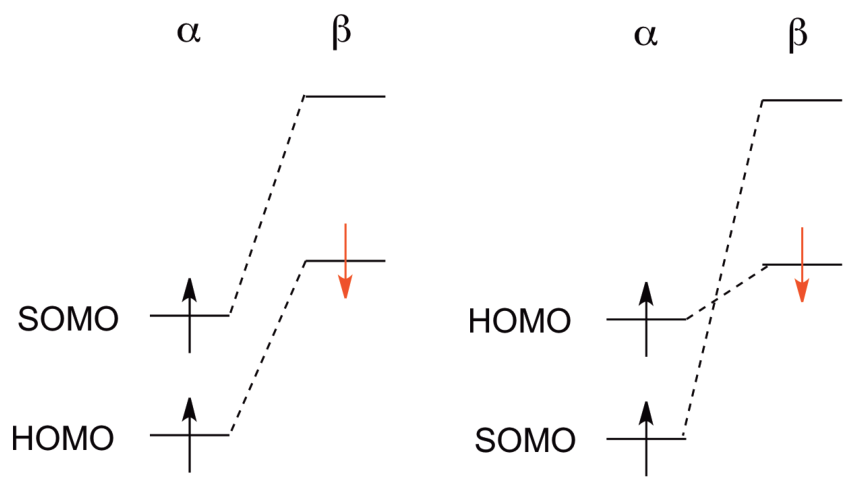
\includegraphics[width=0.78\linewidth]{scheme03_donor_HOMO_spin_polarization.png}}
  \end{columns}
\end{frame}

\begin{frame}{When does the SOMO drop below the HOMO?}
  compare within the $\alpha$ manifold:
  {\large
  \begin{align*}
    \varepsilon_s^\alpha<\varepsilon_h^\alpha
      &\iff h_s+2J_{hs}\canc<2->{-K_{hs}}<h_h+J_{hh}+J_{hs}\canc<2->{-K_{hs}}\\
      &\uncover<3->{\iff h_s+J_{hs}<h_h+J_{hh}}
  \end{align*}}
  \onslide<4->{\small radical orbital: its energy plus repulsion with \emph{one} $h$ electron, vs.\ $h$'s energy plus its \emph{self}-repulsion}
  \vskip0.3cm
  \begin{columns}[T]
    \column{0.48\textwidth}
    \onslide<5->{\begin{plainpanel}\cgold{favours conversion}: a stable radical (low $h_s$) beside an electron-rich, e.g.\ anionic,
      fragment (high $h_h$)\end{plainpanel}}
    \column{0.48\textwidth}
    \onslide<6->{\begin{paperclaim}``spatially separated stable radical center and molecular fragment serving as a source of
      high-energy doubly occupied orbitals'' (p.\ 454)\end{paperclaim}}
  \end{columns}
\end{frame}

\begin{frame}{The redox fingerprint, derived}
  \begin{columns}[T]
    \column{0.5\textwidth}
    \cgold{oxidation}
    \begin{itemize}
      \item Koopmans: $\mathrm{IP}(h)=-\varepsilon_h<\mathrm{IP}(s)$
      \item<2-> product $s^1h^1$: a diradical
      \item<3-> its states: $E_{\OSS}-E_T=2K_{sh}>0$
      \item<4-> \cgold{triplet} cation diradicals with nondegenerate SOMOs, as observed
    \end{itemize}
    \column{0.47\textwidth}
    \onslide<5->{\cgold{reduction}}
    \begin{itemize}
      \item<5-> into $s\beta$ at $\varepsilon_s^\beta$, or into $l$ at $\varepsilon_l$
      \item<6-> diradical $s^1h^2l^1$ iff $\varepsilon_l<h_s+J_{ss}+2J_{hs}-K_{hs}$
      \item<7-> \crose{a separate condition}: SOMO--HOMO conversion alone does not imply it
    \end{itemize}
    \onslide<8->{\small\cmuted{the large on-site $J_{ss}$ is what pushes $\varepsilon_s^\beta$ up}}
  \end{columns}
\end{frame}

\begin{frame}{ROHF: are these orbital energies even real?}
  \begin{paperclaim}
    ``erroneous non-aufbau occupations can be observed with restricted open-shell methods depending on the
    canonicalization parameters of the $\alpha$ and $\beta$ electrons in Fock matrix'' (p.\ 449)
  \end{paperclaim}
  spaces: core $c$ (doubly), open $o$ ($\alpha$), virtual $v$; \quad $\mathbf D^\alpha=\mathbf D_c+\mathbf D_o$, \ $\mathbf D^\beta=\mathbf D_c$
  {\large
  \[
    \uncover<2->{\delta E=\operatorname{tr}(\mathbf F^\alpha\delta\mathbf D^\alpha)+\operatorname{tr}(\mathbf F^\beta\delta\mathbf D^\beta),\qquad
    \text{rotation }p\leftrightarrow q:\ \delta\mathbf D^\sigma=\kappa(\ket p\bra q+\ket q\bra p)}
  \]}
  \onslide<3->{\small\cmuted{a rotation changes $\mathbf D^\sigma$ only if exactly one of $p,q$ is occupied in spin $\sigma$}}
\end{frame}

\begin{frame}{ROHF stationarity, rotation by rotation}
  \centering
  \renewcommand{\arraystretch}{1.3}
  \begin{tabular}{llll}
    \toprule
    rotation & changes $\mathbf D^\alpha$? & changes $\mathbf D^\beta$? & condition\\
    \midrule
    $c\leftrightarrow o$ & no (both $\alpha$-occ.) & yes & $F^\beta_{co}=0$\\
    \onslide<2->{$o\leftrightarrow v$} & \onslide<2->{yes} & \onslide<2->{no (both $\beta$-empty)} & \onslide<2->{$F^\alpha_{ov}=0$}\\
    \onslide<3->{$c\leftrightarrow v$} & \onslide<3->{yes} & \onslide<3->{yes} & \onslide<3->{$F^\alpha_{cv}+F^\beta_{cv}=0$}\\
    \onslide<4->{within $c$, $o$ or $v$} & \onslide<4->{no} & \onslide<4->{no} & \onslide<4->{\crose{none: $\delta E\equiv0$}}\\
    \bottomrule
  \end{tabular}
  \vskip0.25cm
  \onslide<5->{
  \begin{keyresult}
    diagonal blocks are \emph{arbitrary}: any $A\mathbf F^\alpha+(1-A)\mathbf F^\beta$ gives the same energy and density,
    but different orbital energies
  \end{keyresult}}
  \onslide<6->{\small\tick\ \cmuted{T11a: required blocks $<10^{-7}$, others $\sim0.1$ (H$_2$NO, NO$_2$, CH$_3$, allyl); PySCF's Roothaan Fock uses exactly these off-diagonal blocks}}
\end{frame}

\begin{frame}{How arbitrary? H$_2$NO, ROHF/6-31G*}
  \begin{columns}[c]
    \column{0.56\textwidth}
    \begin{tikzpicture}
      \begin{axis}[noirplot,width=7.4cm,height=5.4cm,xmin=-0.2,xmax=1.4,ymin=-0.62,ymax=0.32,
          xlabel={weight $A$ in $\mathbf R_{oo}=A\mathbf F^\alpha+(1-A)\mathbf F^\beta$},ylabel={$\varepsilon$ ($\Eh$)},ymajorgrids]
        \addplot[noirgold,very thick,domain=-0.2:1.4] {-0.4666};
        \node[font=\scriptsize,text=noirgold,anchor=south west] at (axis cs:-0.18,-0.46) {HOMO (closed)};
        \addplot[noircyan,very thick,domain=-0.2:1.4] {0.2028+(-0.4397-0.2028)*x};
        \node[font=\scriptsize,text=noircyan,anchor=south west] at (axis cs:0.05,0.13) {SOMO};
        \only<2->{\fill[noirrose] (axis cs:1.042,-0.4666) circle (2.2pt);
          \draw[noirrose,dashed] (axis cs:1.042,-0.62) -- (axis cs:1.042,0.32);
          \node[font=\scriptsize,text=noirrose,anchor=west] at (axis cs:1.06,-0.2) {$A^*\approx1.04$};}
        \only<3->{\fill[noirmuted,opacity=0.15] (axis cs:0,-0.62) rectangle (axis cs:1,0.32);}
      \end{axis}
    \end{tikzpicture}
    \column{0.4\textwidth}
    \begin{itemize}
      \item energy identical for every $A$: $-130.369709\,\Eh$
      \item<2-> SOMO crosses the HOMO at $A^*\approx1.04$
      \item<3-> shaded: the ``natural'' range $0\le A\le1$, no crossing here
    \end{itemize}
    \onslide<4->{\warnpill\ \small the review is right in principle; for ordinary radicals the standard choices do not flip}
  \end{columns}
\end{frame}

\begin{frame}{Hence: trust observables}
  \begin{paperclaim}
    ``a rigorous support for the non-aufbau occupation can be obtained a posteriori from the ionization potentials and
    electron affinities (or redox potentials in solution) \dots\ as well as from the determination of the spin state and
    magnetic properties of the corresponding open-shell oxidation/reduction products.'' (p.\ 449)
  \end{paperclaim}
  \vskip0.3cm
  \centering
  \begin{tikzpicture}
    \node[noirbox=noirrose] (orb) at (0,0) {orbital ordering\\{\scriptsize convention-dependent}};
    \node[noirbox=noirgreen] (obs) at (6,0) {$E(\text{diradical})$ vs\\$E(\text{closed shell})$\\{\scriptsize invariant}};
    \onslide<2->{\draw[noirarr] (orb) -- node[above,font=\scriptsize]{replace by} (obs);}
  \end{tikzpicture}
  \vskip0.3cm
  \onslide<3->{\small this is exactly the test we ran on a distonic radical anion (a few slides ahead)}
\end{frame}

\begin{frame}{Inorganic precedents (Scheme 2)}
  \begin{columns}[c]
    \column{0.36\textwidth}
    \centering
    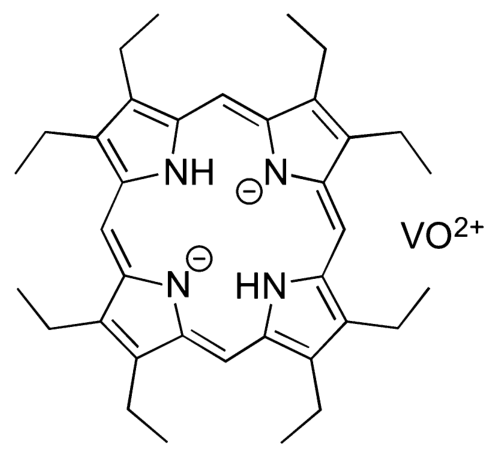
\includegraphics[width=0.85\linewidth]{scheme02_VO_oep.png}\\
    {\scriptsize VO(oep)}
    \column{0.6\textwidth}
    \begin{itemize}
      \item unpaired electron localised on \cgold{vanadium}
      \item<2-> one-electron \emph{oxidation} uses an occupied \cgold{porphyrin} orbital
      \item<3-> one-electron \emph{reduction} uses an unoccupied \cgold{porphyrin} orbital
    \end{itemize}
    \onslide<4->{\small also reported: quantum dots, the LiF dissociation curve}
  \end{columns}
\end{frame}

\begin{frame}{A TEMPO-dithiolate on platinum (Figure 11)}
  \begin{columns}[c]
    \column{0.55\textwidth}
    \centering
    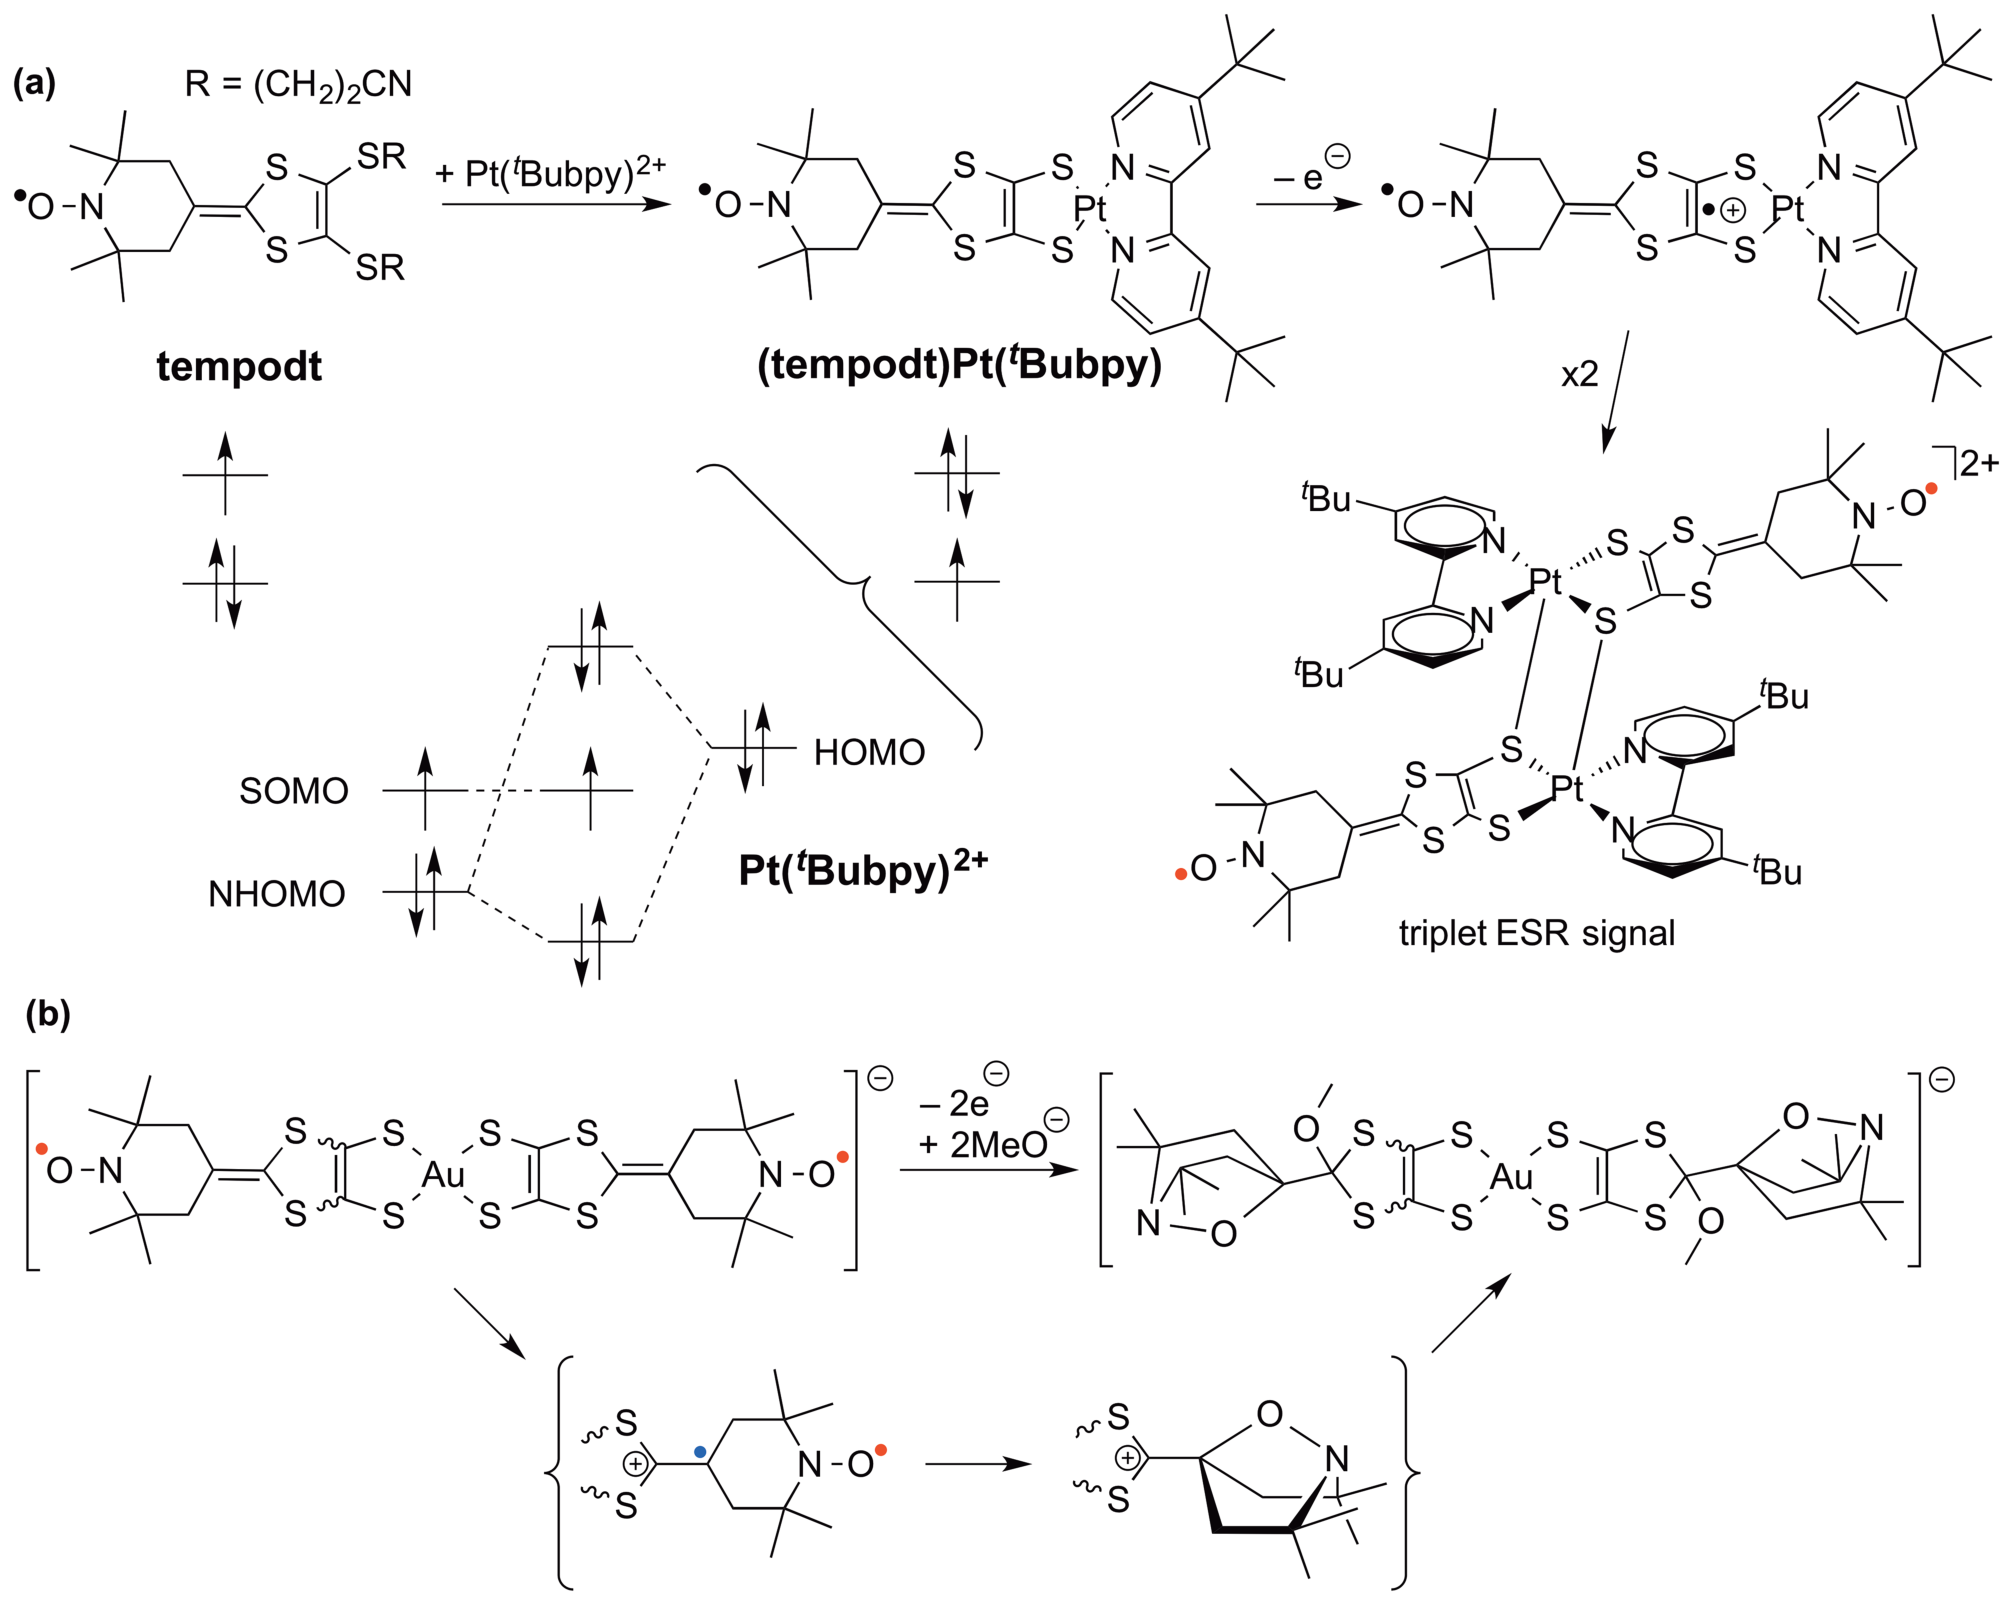
\includegraphics[width=\linewidth]{fig11_tempo_dithiolate_non_aufbau.png}
    \column{0.42\textwidth}
    \small
    \begin{itemize}
      \item oxidation of (tempodt)Pt(tBubpy) removes an electron from the \cgold{dithiolate HOMO}
      \item<2-> evidence: UV--Vis, ESR, CV, DFT and the dimerisation product
      \item<3-> free tempodt is a normal radical; the conversion comes from an antibonding interaction of its NHOMO with the HOMO
        of Pt(tBubpy)$^{2+}$
      \item<4-> (b) a ditempo metalladithiolene: oxidation-generated biradicals couple to a bicyclic product
    \end{itemize}
  \end{columns}
\end{frame}

\begin{frame}{Spin-polarised donors (Figures 12, 13)}
  \begin{columns}[c]
    \column{0.42\textwidth}
    \centering
    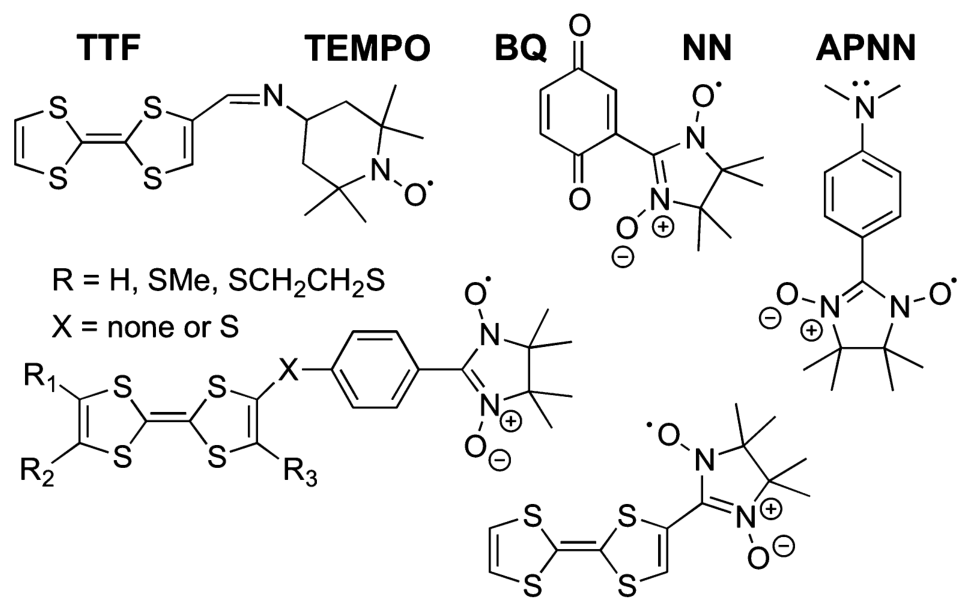
\includegraphics[width=\linewidth]{fig12_nitronyl_nitroxide_donors.png}
    \vskip0.1cm
    \small nitronyl nitroxide (NN) radicals on TTF, BQ, amine donors: one-electron oxidation gives \cgold{triplet cation diradicals}
    \column{0.55\textwidth}
    \onslide<2->{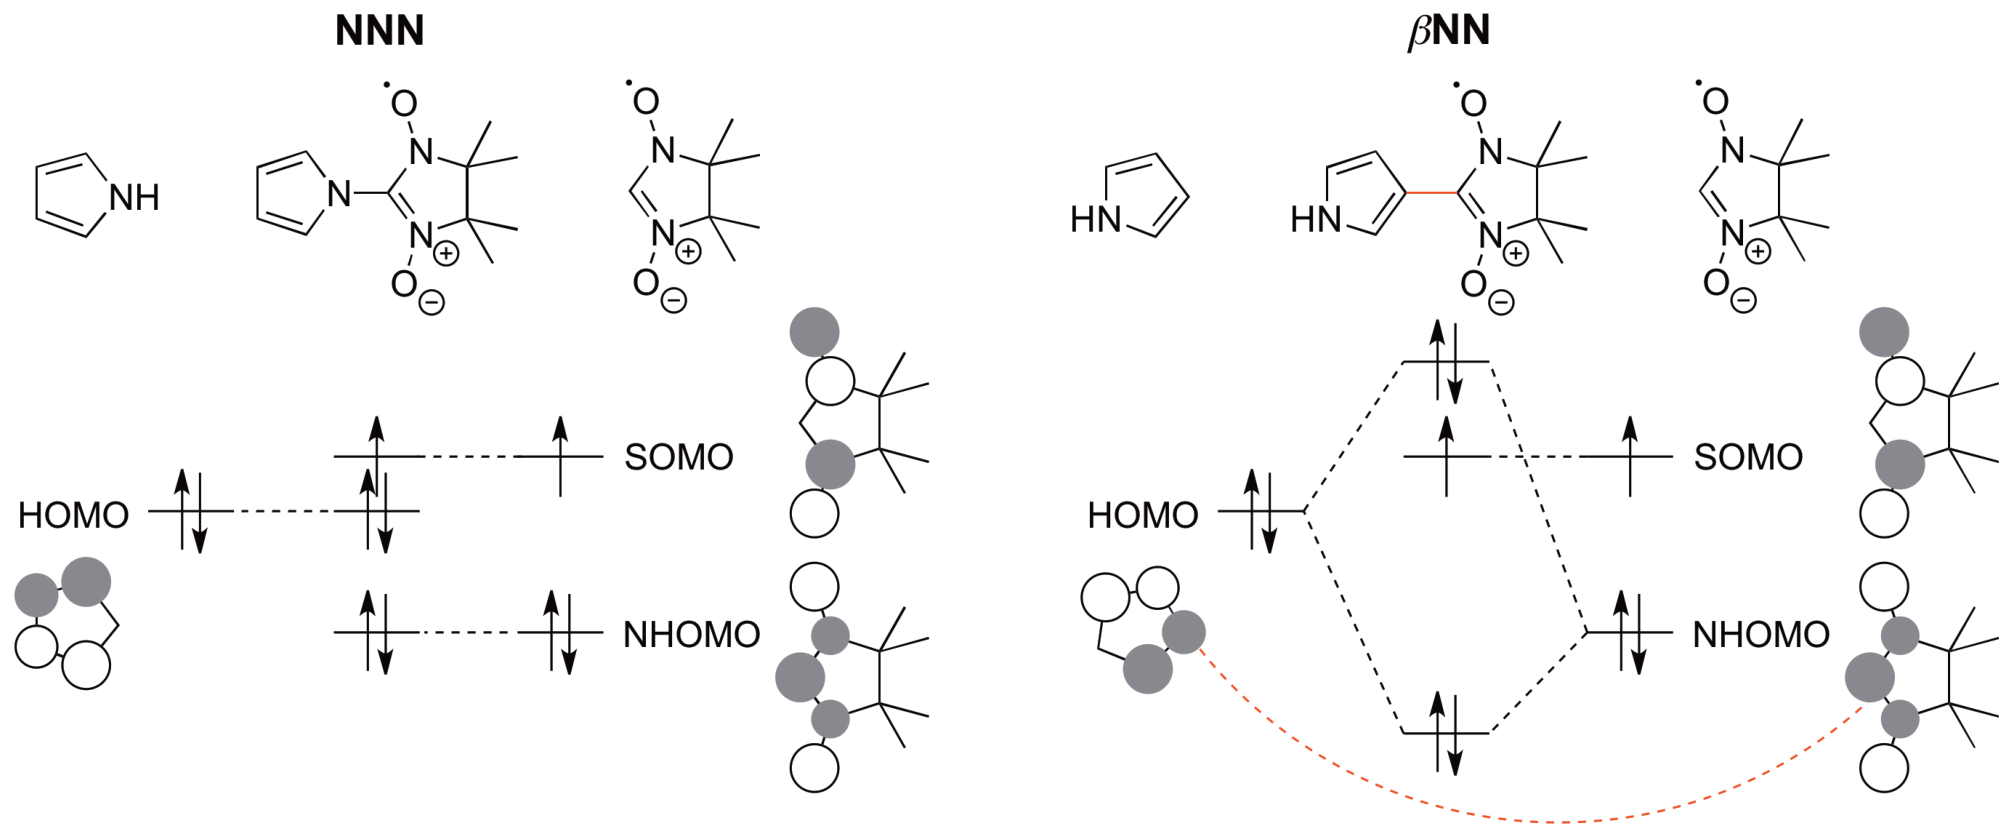
\includegraphics[width=\linewidth]{fig13_disjoint_nondisjoint_orbital_conversion.png}}
    \onslide<3->{\small \cgold{NNN} (1-pyrrolyl): donor HOMO disjoint from SOMO/NHOMO. \cgold{$\beta$NN} (3-pyrrolyl): donor HOMO and NHOMO
      nondisjoint; their combination rises above the SOMO.}
  \end{columns}
\end{frame}

\begin{frame}{Conducting magnets (Scheme 4, Figure 14, Scheme 5)}
  \begin{columns}[c]
    \column{0.5\textwidth}
    \centering
    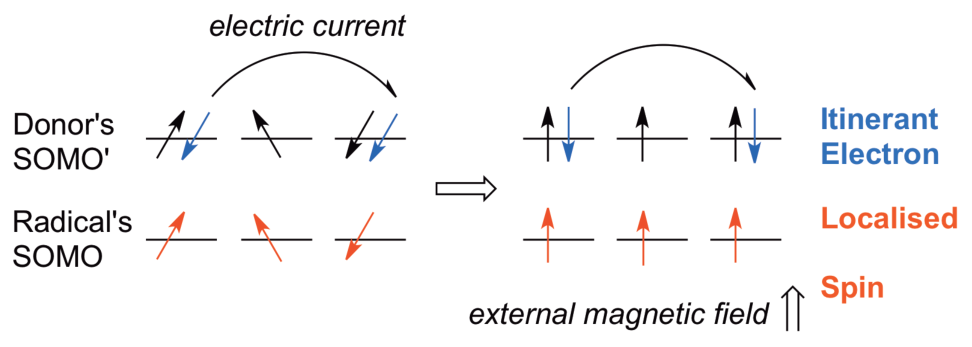
\includegraphics[width=\linewidth]{scheme04_conductivity_magnetism.png}
    \vskip0.1cm
    \only<2-3>{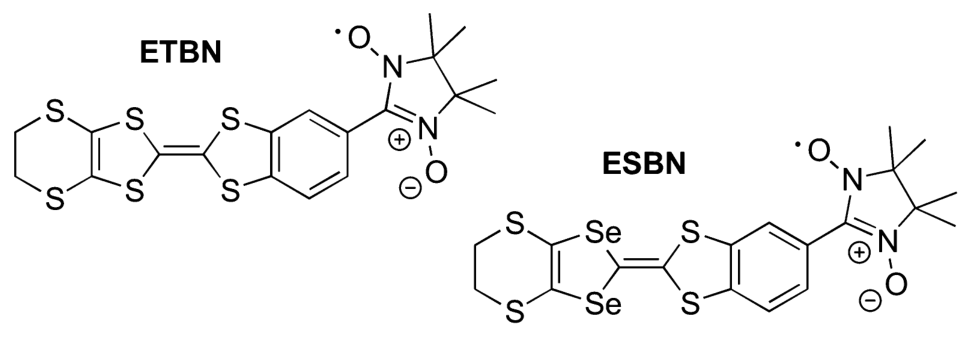
\includegraphics[width=0.8\linewidth]{scheme05_conducting_magnets_ETBN_ESBN.png}}
    \only<4->{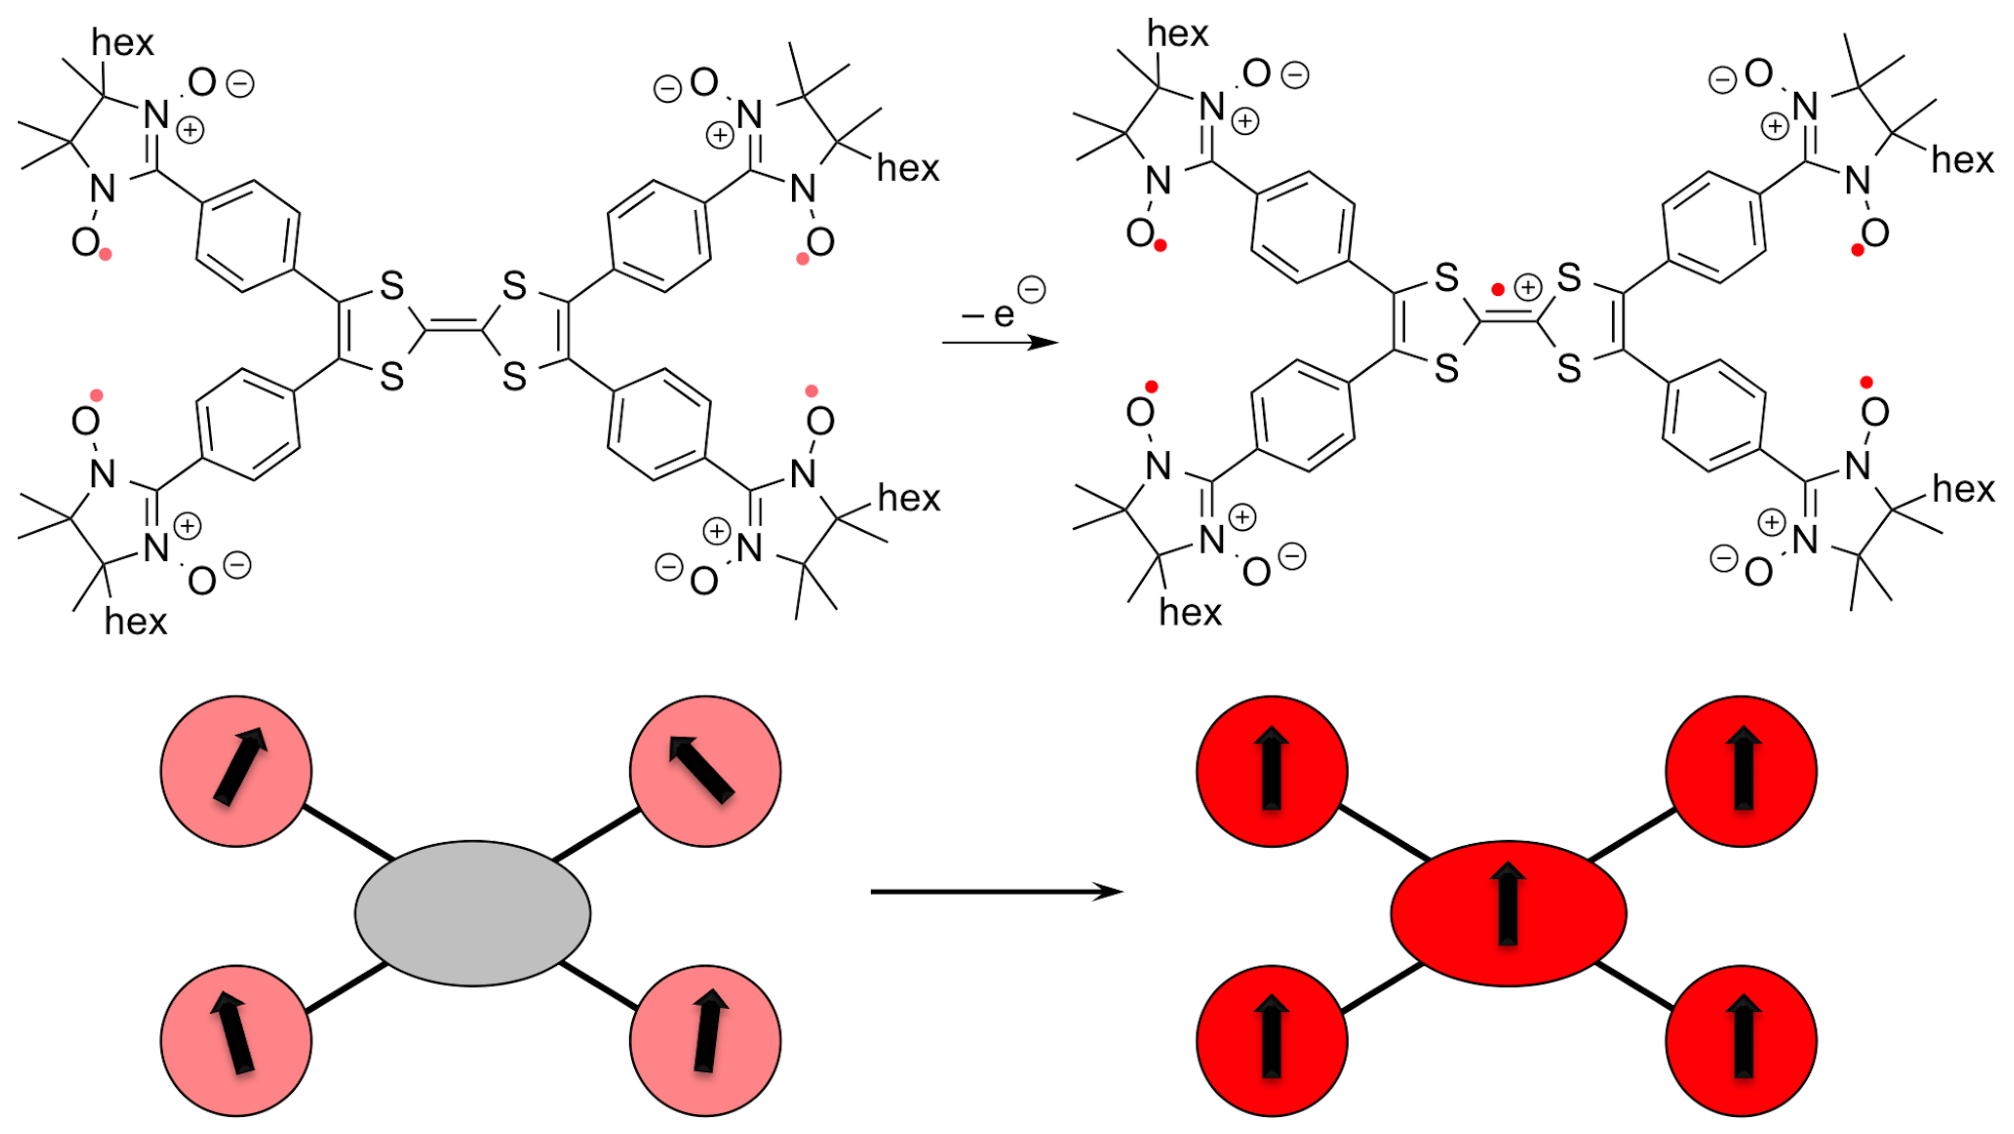
\includegraphics[width=0.95\linewidth]{fig14_oxidation_induced_ferromagnetic_coupling.png}}
    \column{0.47\textwidth}
    \small
    \begin{itemize}
      \item two nondegenerate SOMOs: the donor's (higher) carries an itinerant electron, the radical's (lower) a localised spin
      \item<2-> ETBN, ESBN perchlorate salts: ``first genuine paramagnetic conductors''
      \item<3-> neutral crystals: negative magnetoresistance; field-effect transistors
      \item<4-> Fig.\ 14: several radicals on one donor; oxidation gives a strongly ferromagnetic high-spin system
    \end{itemize}
  \end{columns}
\end{frame}

\begin{frame}{Other radicals, and a pH sensor (Figure 15)}
  \begin{columns}[c]
    \column{0.4\textwidth}
    \centering
    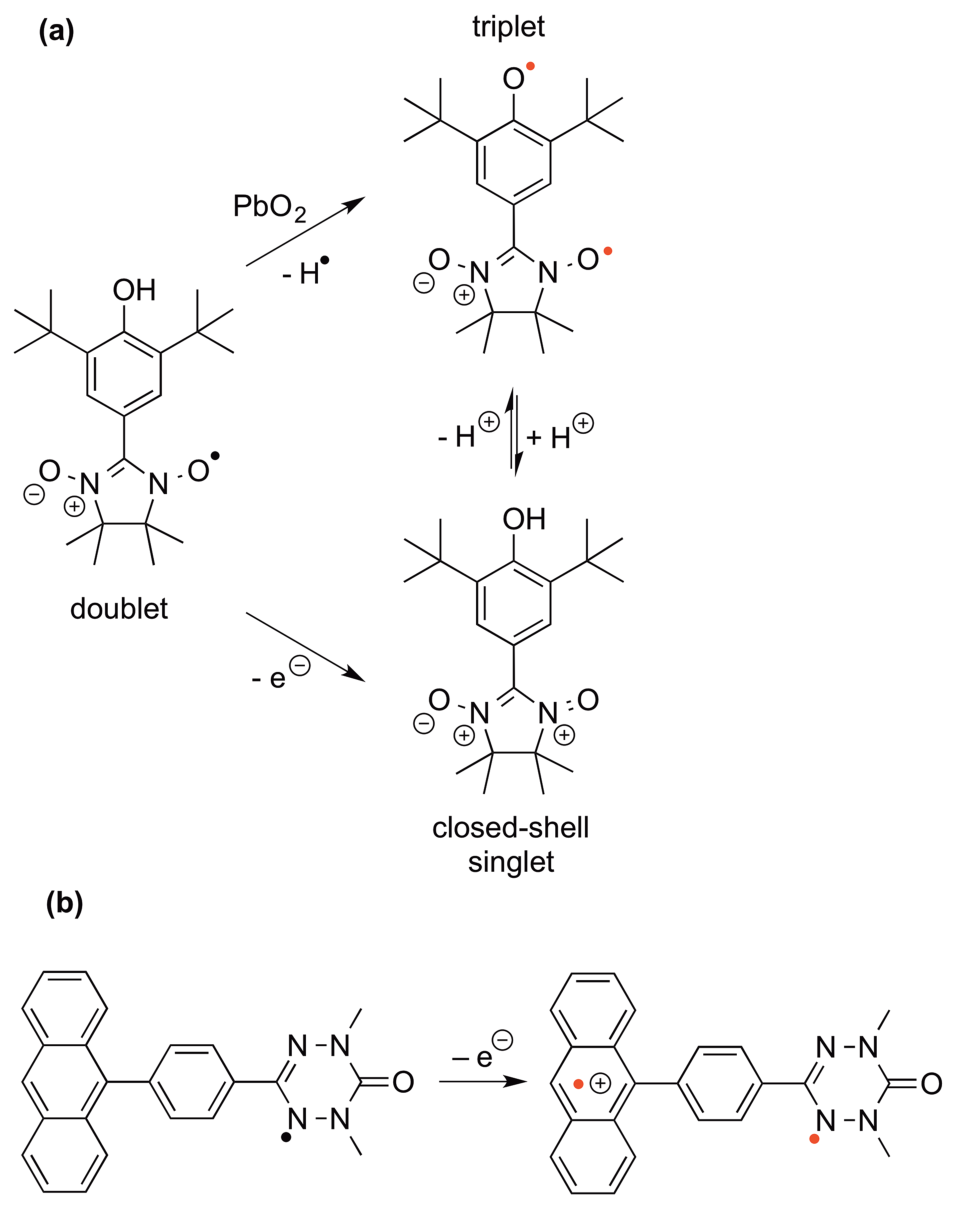
\includegraphics[height=0.66\textheight]{fig15_donors_other_radicals.png}
    \column{0.57\textwidth}
    \begin{itemize}
      \item \cgold{(a)} NN with a phenol-based donor: (de)protonation switches between \emph{triplet} and \emph{closed-shell singlet}:
        a pH sensor
      \item<2-> \cgold{(b)} anthracene--$p$-phenylene--oxoverdazyl (AnOV): high-spin oxidation products
    \end{itemize}
  \end{columns}
\end{frame}

\begin{frame}{Distonic radical anions (Figure 16)}
  \begin{columns}[c]
    \column{0.38\textwidth}
    \centering
    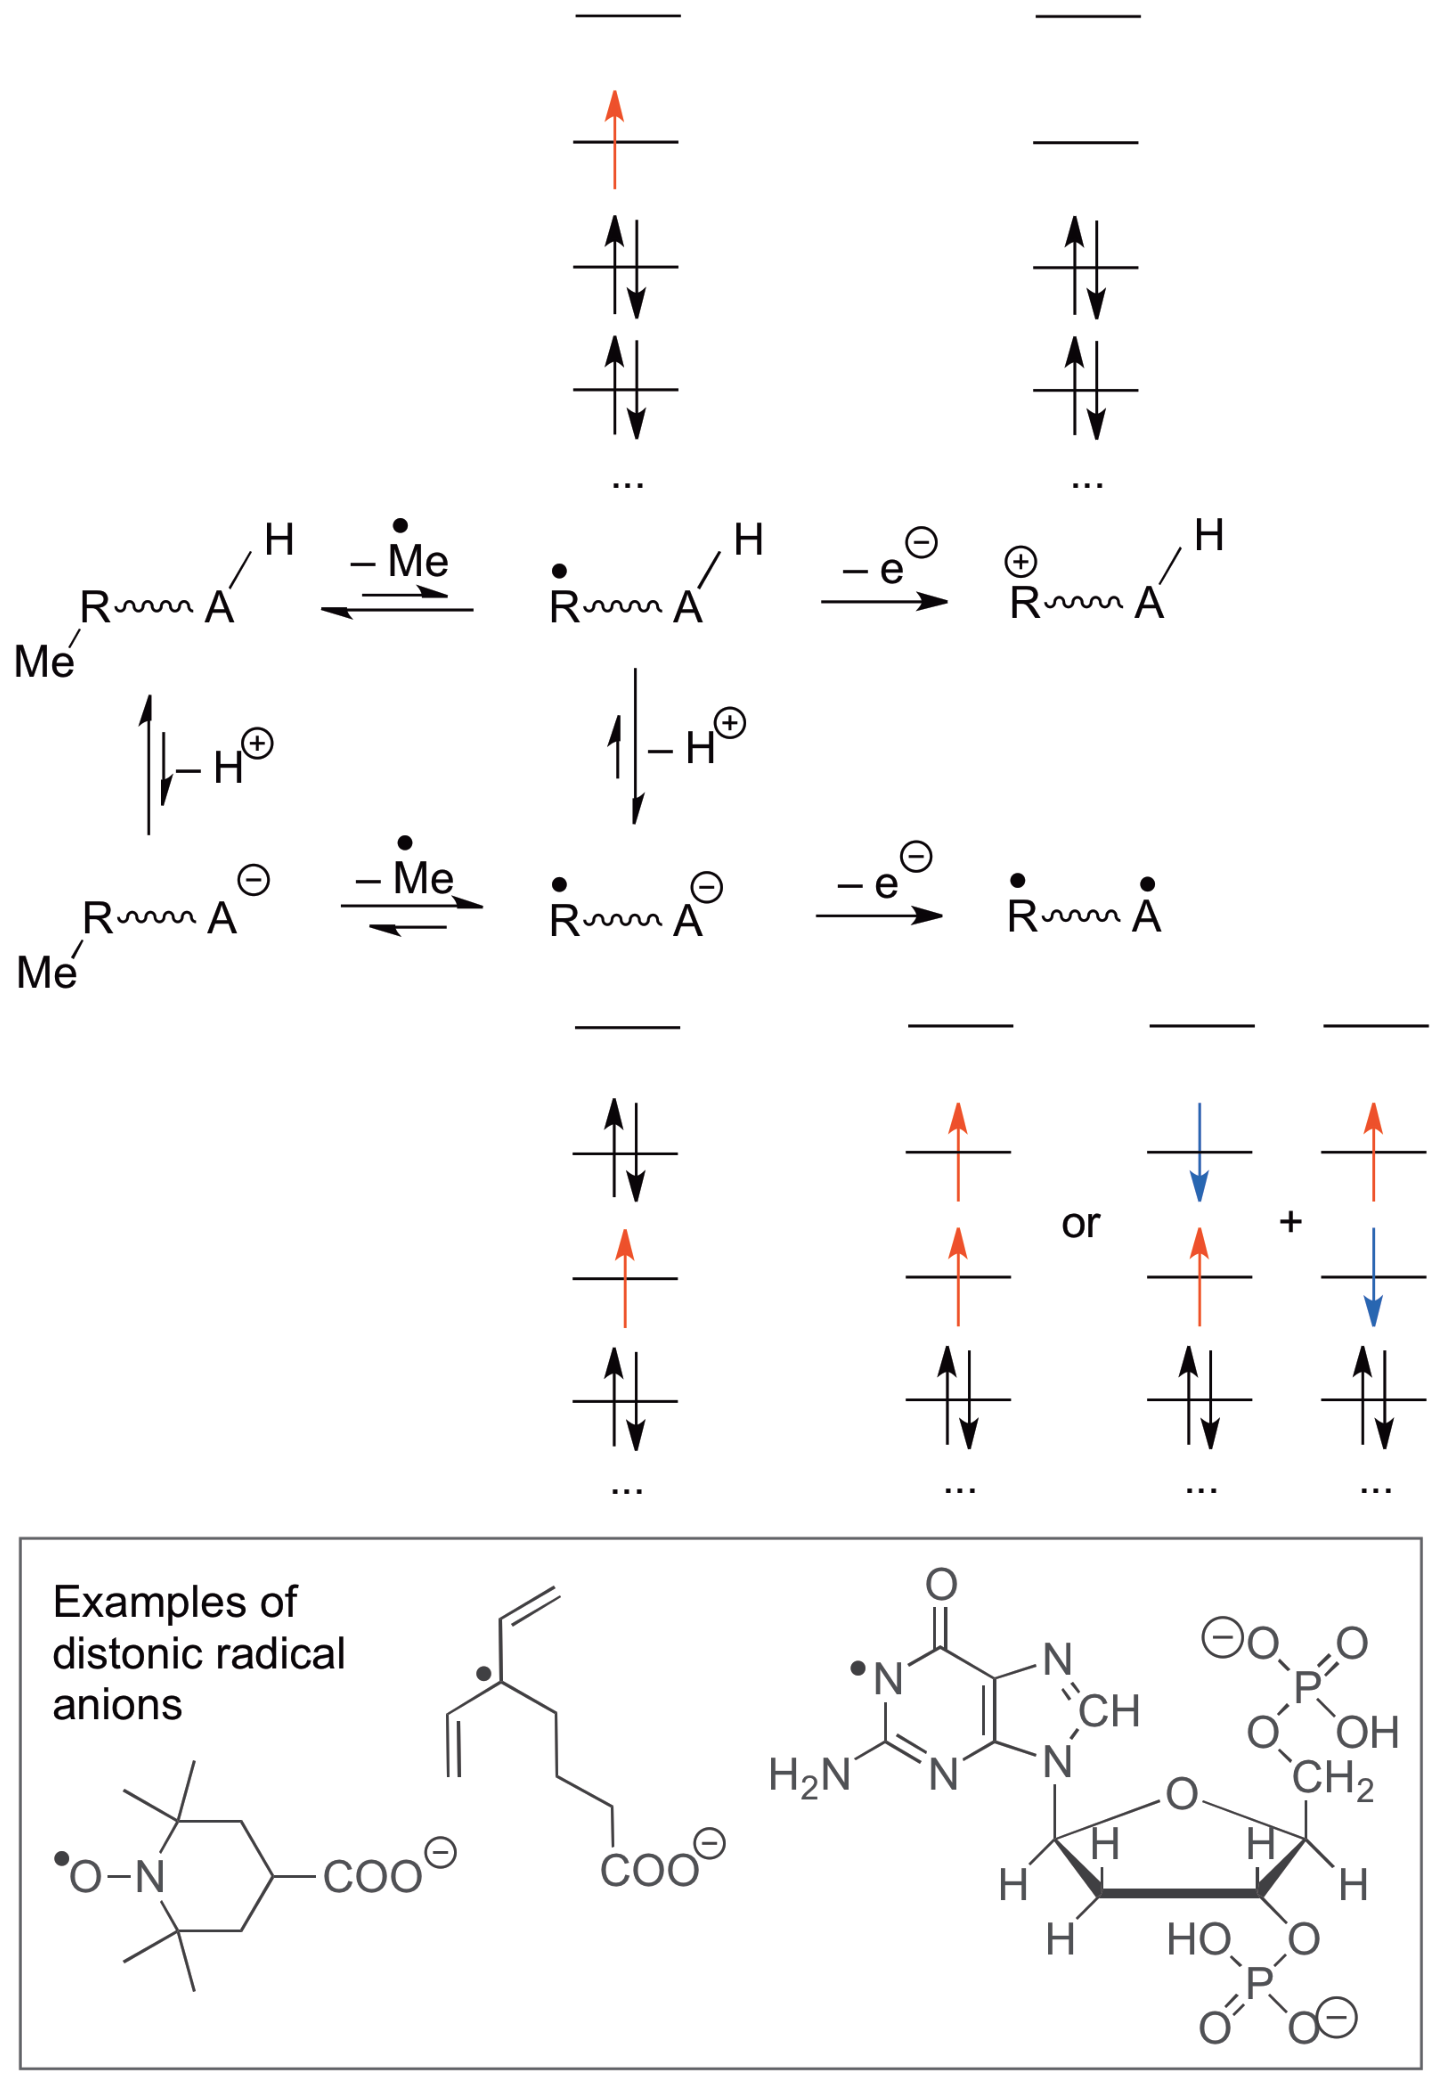
\includegraphics[height=0.78\textheight]{fig16_distonic_radical_anions.png}
    \column{0.59\textwidth}
    \begin{paperclaim}
      a stabilised radical plus an anionic group not $\pi$-conjugated to it: the anion's HOMO lies above the SOMO;
      ``if the anion is protonated, the aufbau orbital occupation is restored'', switchable ``via changing pH''; on oxidation
      the conversion ``yield[s] diradical species preferentially over the closed-shell zwitterion'' (p.\ 452--453)
    \end{paperclaim}
    \onslide<2->{\small \cgold{testable}: compute both oxidised states, with and without the proton}
  \end{columns}
\end{frame}

\begin{frame}{Our test: two radicals, two protonation states, two functionals}{T11/T11c: UB3LYP/6-31G* geometries, vertical oxidation at 6-31+G*}
  \begin{columns}[c]
    \column{0.58\textwidth}
    \begin{tikzpicture}
      \begin{axis}[noirplot,ybar,width=7.8cm,height=5.4cm,bar width=11pt,ymin=-0.6,ymax=1.6,
          symbolic x coords={shortacid,shortanion,tempoacid,tempoanion},xtick=data,
          xticklabels={short acid,short anion,TEMPO acid,TEMPO anion},
          ylabel={$E_T-E_{\text{CS}}$ (eV)},ymajorgrids,legend style={at={(0.5,1.03)},anchor=south,legend columns=2},
          x tick label style={font=\tiny},enlarge x limits=0.18,unbounded coords=discard]
        \addplot[fill=noirgold,draw=none,bar shift=-6pt] table[x=system,y=b3lyp,col sep=comma]{data/distonic.csv};
        \addlegendentry{B3LYP}
        \only<2->{\addplot[fill=noircyan,draw=none,bar shift=6pt] table[x=system,y=camb3lyp,col sep=comma]{data/distonic.csv};}
        \only<2->{\addlegendentry{CAM-B3LYP}}
        \draw[noirfg] (axis cs:shortacid,0) -- (axis cs:tempoanion,0);
      \end{axis}
    \end{tikzpicture}
    \column{0.38\textwidth}
    \small
    $<0$: oxidation gives the \cgreen{diradical}\\
    $>0$: the closed shell
    \begin{itemize}
      \item<1-> acids: closed shell by $1.2$--$1.4$ eV, SOMO $=$ HOMO
      \item<2-> anions, CAM-B3LYP: \cgreen{diradical} by $0.36$ and $0.30$ eV
      \item<3-> anions, B3LYP: misses by $\sim0.07$ eV
    \end{itemize}
  \end{columns}
\end{frame}

\begin{frame}{What the test says}
  \begin{columns}[T]
    \column{0.48\textwidth}
    \cgreen{reproduced}
    \begin{itemize}
      \item SOMO 2--3 levels below the HOMO in the anions; equal to the HOMO in the acids
      \item<2-> protonation moves $E_T-E_{\text{CS}}$ by $\sim1.2$--$1.8$ eV
      \item<3-> with CAM-B3LYP, the anions oxidise to diradicals: \okpill
    \end{itemize}
    \column{0.48\textwidth}
    \onslide<4->{\cgold{caveat}}
    \begin{itemize}
      \item<4-> B3LYP lowers the closed shell by $0.61$ eV vs.\ CAM-B3LYP, the triplet by only $0.17$
      \item<5-> verdict flips at $\sim0.07$ eV: a functional-sensitive claim
      \item<6-> delocalisation error is a plausible cause (not tested)
    \end{itemize}
  \end{columns}
\end{frame}

\begin{frame}{Non-aufbau by electron addition (Figure 17)}
  \begin{columns}[c]
    \column{0.52\textwidth}
    \centering
    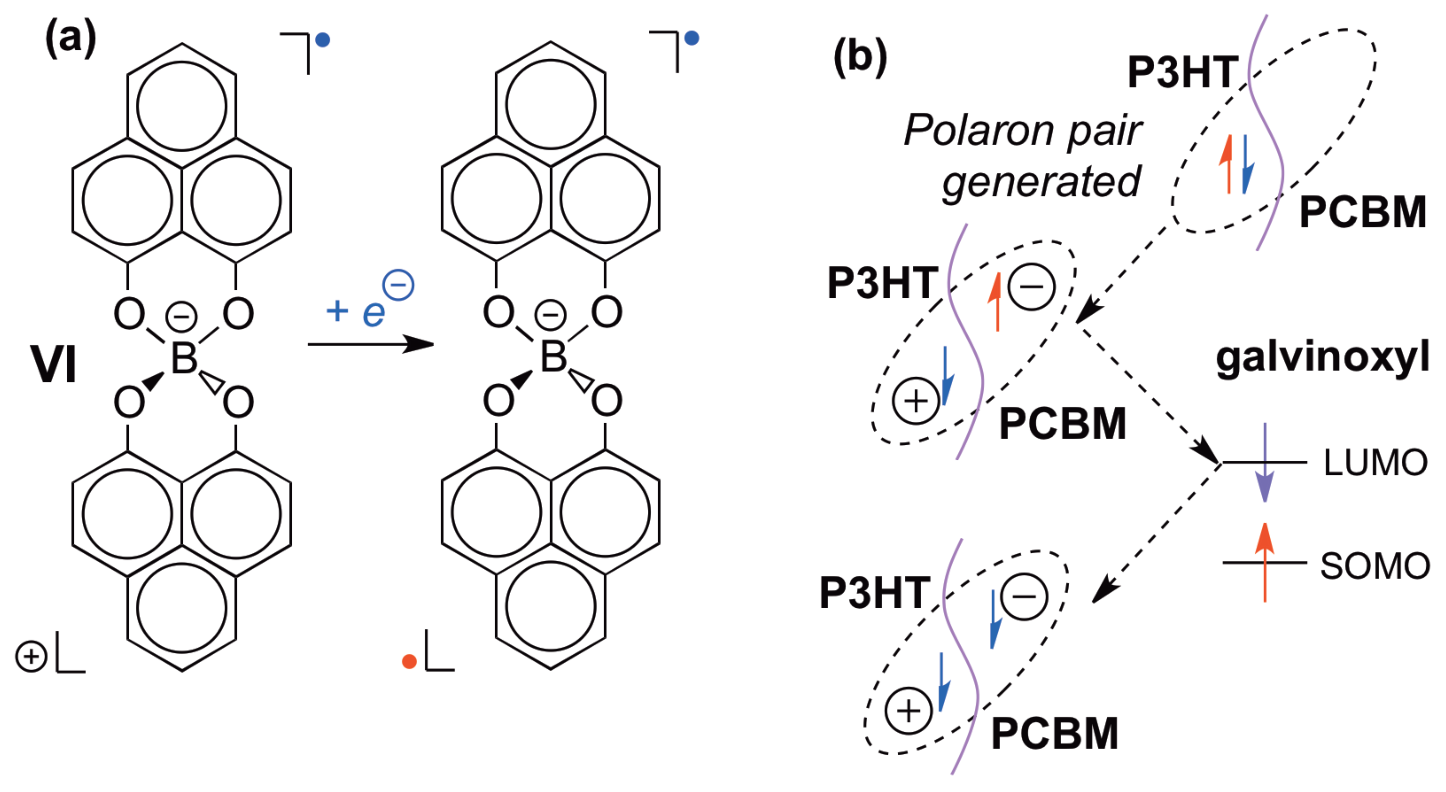
\includegraphics[width=\linewidth]{fig17_non_aufbau_by_electron_addition.png}
    \column{0.45\textwidth}
    \small
    \begin{itemize}
      \item \cgold{(a)} spirobiphenalenyl VI is reduced to an open-shell singlet; it crystallises without dimerising: an intrinsic
        molecular metal
      \item<2-> \cgold{(b)} galvinoxyl in P3HT/PCBM: its LUMO mediates singlet$\to$triplet crossing of polaron pairs via exchange,
        preventing recombination and raising photovoltaic efficiency
      \item<3-> self-doping: in TTFCOO$^-$NH$_4^+$ the SOMO of TTF$^{+\bullet}$ is not the highest occupied orbital
    \end{itemize}
  \end{columns}
\end{frame}

% ============================================================ broken symmetry and spin projection
\section{Broken symmetry}

\begin{frame}{Cheap methods for diradicals}
  \begin{paperclaim}
    ``relatively `cheap' methods such as unrestricted or broken symmetry formalisms suffer from a number of serious
    drawbacks, while rigorous methods \dots\ are generally not feasible for systems large enough to be practically
    valuable.'' (p.\ 443)
  \end{paperclaim}
  \begin{columns}[c]
    \column{0.55\textwidth}
    broken-symmetry (BS) determinant $\ket{a'\bar b'}$, \ $a'$ on centre $l$, $b'$ on $r$, overlap $s=\braket{a'}{b'}$
    {\large
    \begin{align*}
      \uncover<2->{\ev{\hat S^2}_{\text{UHF}}}&\uncover<2->{=S_z(S_z+1)+N_\beta-\textstyle\sum_{i\alpha,j\beta}|\braket ij|^2}\\
      \uncover<3->{\ev{\hat S^2}_{\text{BS}}}&\uncover<3->{=0+1-s^2}
    \end{align*}}
    \column{0.4\textwidth}
    \onslide<4->{\small $s=1$: closed shell, $\ev{\hat S^2}=0$\\ $s=0$: half singlet, half triplet, $\ev{\hat S^2}=1$}\\[4pt]
    \onslide<5->{\cgold{a single determinant cannot be the open-shell singlet} (Part III)}
  \end{columns}
\end{frame}

\begin{frame}{Yamaguchi's projection, derived}
  \begin{assume}
    two-centre Heisenberg model $\hat H=-2J\,\hat{\mathbf S}_1\!\cdot\!\hat{\mathbf S}_2$; BS state $=c_S\Psi_S+c_T\Psi_T$ ($M_S=0$)
  \end{assume}
  {\large
  \begin{align*}
    \stepno{1}\ \hat{\mathbf S}_1\!\cdot\!\hat{\mathbf S}_2&=\tfrac12\bigl[S(S+1)-\tfrac32\bigr]
      \ \Rightarrow\ E_T=-\tfrac J2,\ E_S=\tfrac{3J}2,\ E_S-E_T=2J\\
    \uncover<2->{\stepno{2}\ \ev{\hat S^2}_{\text{BS}}}&\uncover<2->{=2|c_T|^2,\qquad E_{\text{BS}}=|c_S|^2E_S+|c_T|^2E_T}\\
    \uncover<3->{\stepno{3}\ E_{\text{BS}}-E_T}&\uncover<3->{=|c_S|^2(E_S-E_T)=\bigl(1-\tfrac12\ev{\hat S^2}_{\text{BS}}\bigr)2J}\\
    \uncover<4->{\stepno{4}\ J}&\uncover<4->{=\dfrac{E_{\text{BS}}-E_{\text{HS}}}{\ev{\hat S^2}_{\text{HS}}-\ev{\hat S^2}_{\text{BS}}}\qquad(\ev{\hat S^2}_{\text{HS}}=2)}
  \end{align*}}
  \onslide<5->{\centering\small\cmuted{Lean: \texttt{yamaguchi}; sign conventions differ between sources, here $J<0$ is antiferromagnetic}\par}
\end{frame}

\begin{frame}{How good is it? The Hubbard dimer}{T14: self-consistent BS-UHF vs the exact singlet--triplet gap}
  \begin{columns}[c]
    \column{0.58\textwidth}
    \begin{tikzpicture}
      \begin{axis}[noirplot,width=7.6cm,height=5.4cm,xmin=2,xmax=16,ymin=-0.62,ymax=0,
          xlabel={$U/t$},ylabel={$J/t$},ymajorgrids,legend pos=south east]
        \addplot[noircyan,very thick] table[x=U,y=Jexact,col sep=comma]{data/yamaguchi.csv};
        \addlegendentry{exact $\tfrac14(U-\sqrt{U^2+16t^2})$}
        \only<2->{\addplot[noirgold,very thick,dashed] table[x=U,y=Jyam,col sep=comma]{data/yamaguchi.csv};}
        \only<2->{\addlegendentry{Yamaguchi from BS-UHF}}
      \end{axis}
    \end{tikzpicture}
    \column{0.38\textwidth}
    \begin{itemize}
      \item<2-> $U=3t$: error $-7.7\%$
      \item<3-> $U=12t$: $-0.1\%$
      \item<4-> good when the centres are weakly coupled ($\ev{\hat S^2}_{\text{BS}}\to1$), poor when covalent
    \end{itemize}
    \onslide<5->{\okpill\ \small ``serious drawbacks'' is fair}
  \end{columns}
\end{frame}

% ============================================================ our verification machinery
\section{Our verification}

\begin{frame}{The repository}
  \begin{columns}[c]
    \column{0.5\textwidth}
    \scriptsize
    \begin{tabular}{@{}l l@{}}
      \multicolumn{2}{@{}l}{\cgold{\ttfamily CH5103\_Term\_Paper/}}\\
      \ttfamily\ \ paper/ & \cmuted{the review (PDF)}\\
      \ttfamily\ \ derivations/ & \cmuted{18 LaTeX sections}\\
      \ttfamily\ \ verification/ & \cmuted{T1--T15 scripts, logs, results/}\\
      \ttfamily\ \ \ \ lean\_proofs/ & \cmuted{Lean 4 + Mathlib (T17)}\\
      \ttfamily\ \ assets/ & \cmuted{figures, captions (JSONL)}\\
      \ttfamily\ \ presentation/ & \cmuted{this deck}\\
      \ttfamily\ \ docs/ & \cmuted{findings, test matrix}\\
      \ttfamily\ \ plans/ & \cmuted{working log, audit}\\
      \ttfamily\ \ site/ & \cmuted{web page (GitHub Pages)}\\
      \ttfamily\ \ pyproject.toml, uv.lock & \cmuted{pinned environment}\\
      \ttfamily\ \ Makefile & \cmuted{one command per artefact}
    \end{tabular}
    \column{0.46\textwidth}
    \onslide<2->{
    \begin{plainpanel}
      \ttfamily\footnotesize
      make sync\ \ \ \ \ \ \ \cmuted{\# uv, locked env}\\
      make verify\ \ \ \ \ \cmuted{\# T1--T15 > results/}\\
      make verify-dft\ \cmuted{\# T11, T11c}\\
      make lean\ \ \ \ \ \ \ \cmuted{\# T17}\\
      make derivations\\
      make figures\ \ \ \ \cmuted{\# byte-identical}
    \end{plainpanel}}
    \onslide<3->{\footnotesize Python 3.12 pinned by \texttt{uv.lock}\\ PySCF 2.14, SymPy 1.14\\ Lean 4.29.1, Mathlib 4.29.1}
  \end{columns}
\end{frame}

\begin{frame}{The test matrix (1/2)}
  \centering\small
  \renewcommand{\arraystretch}{1.12}
  \begin{tabular}{llll}
    \toprule
    test & what & method & result\\
    \midrule
    T1 & spin functions, Fig.\ 1 combinations, sign erratum & SymPy & \okpill\\
    T1b & sign erratum again: $\hat S^2$ on numerical tensors & NumPy & \okpill\\
    T2 & $2e/2o$ Hamiltonian vs full CI (5 random sets) & PySCF FCI & \okpill\\
    T3 & $K_{pq}\ge0$, $J_{pq}\ge K_{pq}$ & RHF/6-31G H$_2$O & \okpill\\
    T4 & He $2\,^3S/2\,^1S$: virial, less screening & exact 2-electron & \okpill\\
    T5 & H$_2$ dissociation limits & STO-3G closed forms & \okpill\\
    T6 & two-orbital gap model & SymPy & \okpill\\
    T7 & kinetic exchange, extended dimer & SymPy + FCI & \okpill\\
    T8 & Hückel NBMO rules, disjointness & NumPy & \okpill\\
    T9 & Ovchinnikov/Lieb spins; spin alternation & exact diagonalisation & \okpill\\
    \bottomrule
  \end{tabular}
  \symbolstrip{SymPy: exact symbolic algebra \quad PySCF: quantum-chemistry package \quad FCI: full configuration interaction (exact in the basis)
    \quad RHF: restricted HF \quad 6-31G, STO-3G: basis sets \quad exact diagonalisation: all eigenstates of a model Hamiltonian}
\end{frame}

\begin{frame}{The test matrix (2/2)}
  \centering\small
  \renewcommand{\arraystretch}{1.02}
  \begin{tabular}{llll}
    \toprule
    test & what & method & result\\
    \midrule
    T9b & gap $\propto U$ vs $\propto U^2$ & exact diagonalisation & \okpill\\
    T10 & S--T gap $=$ HOMO difference & SymPy & \okpill\\
    T11a & ROHF stationarity, canonicalisation & ROHF/6-31G* & \okpill\\
    T11b & distonic anion, B3LYP & UB3LYP $\Delta$SCF & \pill{noirrose}{fail}\\
    T11c & distonic anions/acids, two functionals & UKS $\Delta$SCF; \texttt{t11c\_check.py} & \okpill\\
    T12 & 3d/4s identity & SymPy & \okpill\\
    T13 & $[\hat l_1,r_{12}^{-1}]\neq0$, $[\hat L,r_{12}^{-1}]=0$ & SymPy & \okpill\\
    T14 & Yamaguchi projection & BS-UHF dimer & \okpill\\
    T15 & same- vs opposite-spin correlation & MP2, He & \okpill\\
    T17 & 17 algebraic theorems & Lean 4 + Mathlib & \okpill\\
    \bottomrule
  \end{tabular}
  \vskip0.1cm
  {\scriptsize\cmuted{T11b fails as recorded: B3LYP misses the crossover by 0.06--0.07 eV; T11c shows the outcome depends on the functional.
    T16 (citations checked by hand against publisher records) has no script.}}
  \symbolstrip{$\Delta$SCF: energy difference of two separate SCF calculations \quad UKS: unrestricted Kohn--Sham DFT \quad
    MP2: second-order perturbation theory \quad BS-UHF: broken-symmetry unrestricted HF}
\end{frame}

\begin{frame}[fragile]{Inside T4: helium, exact in a 16s7p4d basis}{verification/t03\_t05\_hund\_virial\_h2.py (excerpt, unedited)}
  \inputminted[fontsize=\tiny,firstline=42,lastline=62]{python}{../verification/t03_t05_hund_virial_h2.py}
  \symbolstrip{symmetric $C$ $\leftrightarrow$ singlet, antisymmetric $C$ $\leftrightarrow$ triplet (Part III) \quad \texttt{C[p,q]}: coefficient of $\phi_p(1)\phi_q(2)$
    \quad \texttt{h}, \texttt{T}, \texttt{V}: one-electron, kinetic, nuclear matrices \quad \texttt{eri}: $(pq|rs)$ \quad \texttt{B}: basis of (anti)symmetric pairs
    \quad \texttt{Tex}, \texttt{Vne}, \texttt{Vee}: virial components}
\end{frame}

\begin{frame}[fragile]{Inside T11a: ROHF Fock blocks}{verification/t11\_rohf\_and\_distonic.py (excerpt)}
  \inputminted[fontsize=\scriptsize,firstline=14,lastline=24]{python}{../verification/t11_rohf_and_distonic.py}
  \inputminted[fontsize=\scriptsize,firstline=51,lastline=54]{python}{../verification/t11_rohf_and_distonic.py}
  {\small UHF Fock matrices from the ROHF densities, then the blocks the stationarity table says must vanish}
  \symbolstrip{\texttt{Fa}, \texttt{Fb}: $\mathbf F^\alpha,\mathbf F^\beta$ in the MO basis \quad \texttt{c}, \texttt{o}, \texttt{v}: core, open, virtual
    indices \quad \texttt{g\_*}: blocks that must vanish \quad \texttt{n\_*}: blocks free to be non-zero}
\end{frame}

\begin{frame}[fragile]{Inside T17: Lean proves the less-screening logic}{verification/lean\_proofs/Ch5103/Identities.lean (excerpt)}
  \inputminted[fontsize=\scriptsize,firstline=72,lastline=77]{lean4}{../verification/lean_proofs/Ch5103/Identities.lean}
  \inputminted[fontsize=\scriptsize,firstline=79,lastline=83]{lean4}{../verification/lean_proofs/Ch5103/Identities.lean}
  \onslide<2->{
  \begin{checked}[Axiom audit]
    \texttt{\#print axioms}, all 17 theorems: only \texttt{propext}, \texttt{Classical.choice}, \texttt{Quot.sound}
  \end{checked}}
  \symbolstrip{\texttt{dT}, \texttt{dVne}, \texttt{dVee}, \texttt{dE}: triplet minus singlet \quad \texttt{hvir}: virial theorem for both states
    \quad \texttt{linarith}: proves linear inequalities automatically \quad axioms: the standard three of Lean's logic}
\end{frame}

\begin{frame}{What the tests caught in our own work}
  \begin{columns}[T]
    \column{0.52\textwidth}
    \small
    \begin{itemize}
      \item \cgold{T8}: we assumed $\#\text{NBMO}=N-2T$; cyclobutadiene says $\ge$
      \item<2-> \cgold{T9b}: lowest $S_z=0$ level was the triplet's $M_S=0$ component, not a singlet
      \item<3-> \cgold{T11a}: we expected a SOMO/HOMO flip in standard schemes; it needs $A>1$
      \item<4-> \cgold{T5}: a symmetry tolerance of $10^{-10}$ failed on round-off at $S\sim10^{-16}$
      \item<5-> \cgold{T12}: our illustrative numbers had the wrong sign of $\Delta$
    \end{itemize}
    \column{0.44\textwidth}
    \onslide<6->{
    \begin{keyresult}
      every failure was diagnosed before the test changed, and each is logged in \texttt{plans/tests.md}
    \end{keyresult}}
    \onslide<7->{\small\cmuted{a check that is able to fail is what turns ``I believe'' into ``checked''}}
  \end{columns}
\end{frame}

% ============================================================ verdict, take-home, references
\section{Verdict}

\begin{frame}{Scorecard (1/2): confirmed}
  \centering\small
  \renewcommand{\arraystretch}{1.15}
  \begin{tabular}{p{8.6cm}l}
    \toprule
    claim & verdict\\
    \midrule
    triplet single-, open-shell singlet multi-reference & \okpill\\
    \onslide<2->{less screening, not lower $V_{ee}$, explains Hund's rule} & \onslide<2->{\okpill}\\
    \onslide<3->{static correlation grows as orbital interaction weakens} & \onslide<3->{\okpill}\\
    \onslide<4->{kinetic exchange; disjoint NBMOs; topology / Ovchinnikov rules} & \onslide<4->{\okpill}\\
    \onslide<5->{3d/4s; one-electron quantum numbers not conserved} & \onslide<5->{\okpill}\\
    \onslide<6->{ROHF orbital energies are convention-dependent} & \onslide<6->{\okpill\ \warnpill}\\
    \bottomrule
  \end{tabular}
\end{frame}

\begin{frame}{Scorecard (2/2): qualified or wrong}
  \centering\small
  \renewcommand{\arraystretch}{1.15}
  \begin{tabular}{p{8.6cm}l}
    \toprule
    claim & verdict\\
    \midrule
    distonic anions oxidise to diradicals, switchable by pH & \partpill\\
    \onslide<2->{same-spin correlation ``an order of magnitude'' smaller} & \onslide<2->{\warnpill}\\
    \onslide<3->{aufbau ``violates'' Pauli; aufbau and Hund's rule ``obsolete''} & \onslide<3->{\warnpill}\\
    \onslide<4->{$^1\Psi_{\OSS}=\tfrac12(D_{\text{iii}}+D_{\text{iv}})$ \ (p.\ 441)} & \onslide<4->{\badpill}\\
    \onslide<5->{Katriel \& Pauncz cited as 1975 (it is 1977)} & \onslide<5->{\badpill}\\
    \bottomrule
  \end{tabular}
\end{frame}

\begin{frame}{The errors, once more}
  \begin{columns}[T]
    \column{0.48\textwidth}
    \begin{erratum}[Sign error, p.\ 441]
      $\tfrac12(D_{\text{iii}}\ \crose{+}\ D_{\text{iv}})$ is the $M_S=0$ triplet; the open-shell singlet is
      $\tfrac12(D_{\text{iv}}\ \cgreen{-}\ D_{\text{iii}})$
    \end{erratum}
    \onslide<2->{
    \begin{erratum}[Citation, ref.\ 11]
      Katriel \& Pauncz, \emph{Adv.\ Quantum Chem.}\ 10, 143 is from 1977
    \end{erratum}}
    \column{0.48\textwidth}
    \onslide<3->{
    \begin{paperclaim}[Possible slip, p.\ 445]
      ``triplet ground state, predicted on the basis of disjoint NBMOs'' contradicts the review's own disjoint/nondisjoint rule
    \end{paperclaim}}
    \onslide<4->{\small none of these touches a conclusion: the chemistry of the review stands}
  \end{columns}
\end{frame}

\begin{frame}{Take-home}
  \begin{enumerate}
    \item a spin state is decided by \cgold{correlation}, not by a single term: Hund's rule, aufbau and topology rules are
          theorems of \emph{models}
    \item<2-> the \cgold{virial theorem} settles Hund's rule: the high-spin state wins on nuclear attraction
    \item<3-> \cgold{disjointness} removes first-order exchange; second-order spin polarisation then picks the singlet
    \item<4-> \cgold{orbital energies are not observables}: judge non-aufbau claims by redox energetics
    \item<5-> distonic radical anions \cgold{do} oxidise to diradicals at CAM-B3LYP, \emph{but} B3LYP disagrees by 0.07 eV:
          a sensitive claim
  \end{enumerate}
  \vskip0.3cm
  \onslide<6->{\centering\noircalli\Large\cgold{Even the open-shell singlet in print can fluctuate.}\par}
\end{frame}

\begin{frame}{Key references}
  \scriptsize
  \begin{itemize}
    \item G.\ Gryn'ova, M.\ L.\ Coote, C.\ Corminboeuf, \emph{WIREs Comput.\ Mol.\ Sci.}\ \textbf{5}, 440 (2015)
    \item K.\ Hongo et al., \emph{J.\ Chem.\ Phys.}\ \textbf{121}, 7144 (2004) \quad (carbon, QMC, less screening)
    \item R.\ J.\ Boyd, \emph{Nature} \textbf{310}, 480 (1984)
    \item J.\ Katriel, R.\ Pauncz, \emph{Adv.\ Quantum Chem.}\ \textbf{10}, 143 (1977)
    \item W.\ T.\ Borden, E.\ R.\ Davidson, \emph{J.\ Am.\ Chem.\ Soc.}\ \textbf{99}, 4587 (1977)
    \item A.\ A.\ Ovchinnikov, \emph{Theor.\ Chim.\ Acta} \textbf{47}, 297 (1978)
    \item E.\ H.\ Lieb, \emph{Phys.\ Rev.\ Lett.}\ \textbf{62}, 1201 (1989)
    \item J.\ F.\ Janak, \emph{Phys.\ Rev.\ B} \textbf{18}, 7165 (1978)
    \item A.\ I.\ Krylov, \emph{Chem.\ Phys.\ Lett.}\ \textbf{338}, 375 (2001)
    \item A.\ Balkov\'a, R.\ J.\ Bartlett, \emph{J.\ Chem.\ Phys.}\ \textbf{101}, 8972 (1994)
    \item K.\ R.\ Glaesemann, M.\ W.\ Schmidt, \emph{J.\ Phys.\ Chem.\ A} \textbf{114}, 8772 (2010)
    \item G.\ Gryn'ova, D.\ L.\ Marshall, S.\ J.\ Blanksby, M.\ L.\ Coote, \emph{Nat.\ Chem.}\ \textbf{5}, 474 (2013)
  \end{itemize}
  \vskip0.1cm
  {\cmuted{full access status of every source: derivations, \S17}}
\end{frame}

\begin{frame}[plain,noframenumbering]
  \centering
  \vfill
  {\noircalli\Huge\cgold{Thank you}}
  \vskip0.5cm
  {\noirgaramond\large derivations \textbullet\ code \textbullet\ proofs \textbullet\ slides}\\[4pt]
  {\ttfamily\small github.com/Shuvam-Banerji-Seal/CH5103\_Term\_Paper}
  \vfill
\end{frame}

\end{document}
